%%%%%% Run at command line, run
%%%%%% xelatex grad-sample.tex 
%%%%%% for a few times to generate the output pdf file
\documentclass[12pt,oneside,openright,a4paper]{cpe-english-project}

\usepackage{polyglossia}
\usepackage{float}
\setdefaultlanguage{english}
\setotherlanguage{thai}
\newfontfamily\thaifont[Script=Thai,Scale=1.23]{TH Sarabun New}
\defaultfontfeatures{Mapping=tex-text,Scale=1.0,LetterSpace=0.0}
\setmainfont[Scale=1.0,LetterSpace=0,WordSpace=1.0,FakeStretch=1.0]{Times New Roman}
\emergencystretch=10pt
%\XeTeXlinebreaklocale "th_TH"	
%\XeTeXlinebreakskip = 0pt plus 1pt
%\setmathfont(Digits)[Scale=1.0,LetterSpace=0,FakeStretch=1.0]{Times New Roman}

%%%%%%%%%%%%%%%%%%%%%%%%%%%%%%%%%%%%%%%%%%%%%%%%%%%%%%%%%%%%%%%%%%%
% Customize below to suit your needs 
% The ones that are optional can be left blank. 
%%%%%%%%%%%%%%%%%%%%%%%%%%%%%%%%%%%%%%%%%%%%%%%%%%%%%%%%%%%%%%%%%%%
% First line of title
\def\disstitleone{Generative AI for Traditional Form Converter}   
% Second line of title
% \def\disstitletwo{Project/Indep title line 2 (optional)}   
% Your first name and lastname
\def\dissauthor{Mr. PRAPAKORN BUTYOJANTO}   % 1st member
\def\dissauthortwo{Mr. PHANASORN SRISAYAM}   % 2nd member (optional)
\def\dissauthorthree{Mr. NATTAWUT PIANOK}   % 3rd member (optional)


% The degree that you're persuing..
\def\dissdegree{Bachelor of Engineering} % Name of the degree
\def\dissdegreeabrev{B.Eng} % Abbreviation of the degree
\def\dissyear{2024}                   % Year of submission
\def\thaidissyear{2567}               % Year of submission (B.E.)

%%%%%%%%%%%%%%%%%%%%%%%%%%%%%%%%%%%%%%%%%%%%
% Your project and independent study committee..
%%%%%%%%%%%%%%%%%%%%%%%%%%%%%%%%%%%%%%%%%%%%
\def\dissadvisor{Dr. Kittipong Piyawanno , Ph.D.}  % Advisor
%% Leave this empty if you have no co-advisor
\def\disscoadvisor{} %Optional
\def\disscommitteetwo{Assoc.Prof. Natasha Dejdumrong, D.Tech.Sci.} 
\def\disscommitteethree{Assoc.Prof. Peerapon Siripongwutikorn, Ph.D.}  
\def\disscommitteefour{Naveed Sultan} 

\def\worktype{Project} %%  Project or Independent study
\def\disscredit{3}   %% 3 credits or 6 credits


\def\fieldofstudy{Computer Engineering} 
\def\department{Computer Engineering} 
\def\faculty{Engineering}

\def\thaifieldofstudy{วิศวกรรมคอมพิวเตอร์} 
\def\thaidepartment{วิศวกรรมคอมพิวเตอร์} 
\def\thaifaculty{วิศวกรรมศาสตร์}
 
\def\appendixnames{Appendix} %%% Appendices or Appendix

\def\thaiworktype{ปริญญานิพนธ์} %  Project or research project % 
\def\thaidisstitleone{เว็บแอปพลิเคชัน AI สำหรับการแปลงฟอร์มกระดาษเป็นเว็บฟอร์ม}
\def\thaidissauthor{นายประภากร บุตรโยจันโท}
\def\thaidissauthortwo{นายพณศร ศรีสยาม} %Optional
\def\thaidissauthorthree{นายณัฐวุฒิ เพียนอก} %Optional

\def\thaidissadvisor{ดร. กิตติพงษ์ ปิยะวรรณโณ}
%% Leave this empty if you have no co-advisor
\def\thaidisscoadvisor{} %Optional
\def\thaidisscoadvisortwo{}  % Co-advisor 2 (if any)
\def\thaidisscoadvisorthree{} % Co-advisor 3 (You better be building space rocket or curing cancer at this point)
\def\thaidissdegree{วิศวกรรมศาสตรบัณฑิต}

% Change the line spacing here...
\linespread{1.15}

%%%%%%%%%%%%%%%%%%%%%%%%%%%%%%%%%%%%%%%%%%%%%%%%%%%%%%%%%%%%%%%%
% End of personal customization.  Do not modify from this part 
% to \begin{document} unless you know what you are doing...
%%%%%%%%%%%%%%%%%%%%%%%%%%%%%%%%%%%%%%%%%%%%%%%%%%%%%%%%%%%%%%%%


%%%%%%%%%%%% Dissertation style %%%%%%%%%%%
%\linespread{1.6} % Double-spaced  
%%\oddsidemargin    0.5in
%%\evensidemargin   0.5in
%%%%%%%%%%%%%%%%%%%%%%%%%%%%%%%%%%%%%%%%%%%
%\renewcommand{\subfigtopskip}{10pt}
%\renewcommand{\subfigbottomskip}{-5pt} 
%\renewcommand{\subfigcapskip}{-6pt} %vertical space between caption
%                                    %and figure.
%\renewcommand{\subfigcapmargin}{0pt}

\renewcommand{\topfraction}{0.85}
\renewcommand{\textfraction}{0.1}

\newtheorem{theorem}{Theorem}
\newtheorem{lemma}{Lemma}
\newtheorem{corollary}{Corollary}

\def\QED{\mbox{\rule[0pt]{1.5ex}{1.5ex}}}
\def\proof{\noindent\hspace{2em}{\itshape Proof: }}
\def\endproof{\hspace*{\fill}~\QED\par\endtrivlist\unskip}
%\newenvironment{proof}{{\sc Proof:}}{~\hfill \blacksquare}
%% The hyperref package redefines the \appendix. This one 
%% is from the dissertation.cls
%\def\appendix#1{\iffirstappendix \appendixcover \firstappendixfalse \fi \chapter{#1}}
%\renewcommand{\arraystretch}{0.8}
%%%%%%%%%%%%%%%%%%%%%%%%%%%%%%%%%%%%%%%%%%%%%%%%%%%%%%%%%%%%%%%%
%%%%%%%%%%%%%%%%%%%%%%%%%%%%%%%%%%%%%%%%%%%%%%%%%%%%%%%%%%%%%%%%


\begin{document}
\pdfstringdefDisableCommands{\let\MakeUppercase\relax}
\begin{center}
  
\includegraphics[width=2.8cm]{logo02.jpg}
\end{center}
\vspace*{-1cm}

\maketitlepage
\makesignaturepage 

%%%%%%%%%%%%%%%%%%%%%%%%%%%%%%%%%%%%%%%%%%%%%%%%%%%%%%%%%%%%%%
%%%%%%%%%%%%%%%%%%%%%% English abstract %%%%%%%%%%%%%%%%%%%%%%%
%%%%%%%%%%%%%%%%%%%%%%%%%%%%%%%%%%%%%%%%%%%%%%%%%%%%%%%%%%%%%%
\abstract

\setlength{\parindent}{15pt} The Generative AI for Traditional Form Converter is a project developed through a web application called PaperlessTransform Application, aimed at solving the problem of time-consuming processes involved in converting PDF forms into web applications. This web application leverages artificial intelligence to analyze data types of input labels. As the demand for form conversion continues to increase, system developers are required to analyze a PDF forms structure, design corresponding database structures, create web application interfaces, and develop new systems. These tasks result in significantly increased work time and workload, causing personnel to spend time inefficiently. The goal of this project is to reduce the burden on system developers by automating parts of this workflow. The application is designed to process a PDF file, detect an input fields using parser,  generate an input field data type using AI-powered text analysis, and generate web-based forms accordingly. In addition to form field detection, the system can store form data in a structured format suitable for web deployment, enabling a smoother transition from traditional documents to digital interfaces. The project team has focused on developing a robust system that not only identifies relevant form elements accurately but also simplifies the data handling and form creation process. After testing the web application, results show that it can detect input field within forms and store data at a basic level, demonstrating its practical effectiveness in real-world scenarios. Therefore, it can be concluded that this project addresses the problem of increased work time and inefficiency for system developers, offering an effective tool for automated form conversion and reducing the manual effort required in digitizing traditional forms.
\begin{flushleft}
\begin{tabular*}{\textwidth}{@{}lp{0.8\textwidth}}
\textbf{Keywords}: & Web Application / Database Design

\end{tabular*}
\end{flushleft}
\endabstract

%%%%%%%%%%%%%%%%%%%%%%%%%%%%%%%%%%%%%%%%%%%%%%%%%%%%%%%%%%%%%%
%%%%%%%%%% Thai abstract here %%%%%%%%%%%%%%%%%%%%%%%%%%%%%%%%%
%%%%%%%%%%%%%%%%%%%%%%%%%%%%%%%%%%%%%%%%%%%%%%%%%%%%%%%%%%%%%%
{
%\begin{thai}
\XeTeXlinebreaklocale "th_TH"	
\XeTeXlinebreakskip = 0pt plus 1pt
\thaifont
\thaiabstract

Generative AI for Traditional Form Converter เป็นโครงการที่จัดทำขึ้นผ่านการพัฒนาผ่านเว็บแอปพลิเคชั่นในชื่อ PaperlessTransform Application
เพื่อแก้ไขปัญหาการใช้ระยะเวลานานในการแปลงแบบฟอร์มกระดาษเป็นรูปแบบเว็บแอปพลิเคชัน โดยการพัฒนาเว็บแอปพลิเคชันนี้ได้มีการใช้ประยุกต์ใช้ปัญญาประดิษฐ์สำหรับการวิเคราะห์เกี่ยวกับประเภทของข้อมูลของคำถาม 
ตามความต้องการที่เพิ่มขึ้นของการแปลงแบบฟอร์ม ดังนั้นนักพัฒนาระบบจึงจำเป็นต้องวิเคราะห์แบบฟอร์มและออกแบบระบบฐานข้อมูลพร้อมทั้งการออกแบบหน้าเว็บแอปพลิเคชัน รวมไปถึงการพัฒนาระบบขึ้นมาใหม่
จึงส่งผลให้ต้องใช้ระยะเวลาในการทำงานที่เพิ่มขึ้น นอกจากนี้ นักพัฒนาระบบต้องเผชิญกับปัญหาภาระงานที่มากขึ้น ส่งผลให้บุคคลากรใช้เวลาในการทำงานอย่างไม่มีประสิทธิภาพ 
โดยโครงการของเรามุ่งเน้นการพัฒนาเว็บแอปพลิเคชันที่สามารถแปลงเอกสารในรูปแบบไฟล์อิเล็กทรอนิกส์ให้เป็นรูปแบบของเว็บแอปพลิเคชัน 
โดยนำข้อความจากไฟล์อิเล็กทรอนิกส์ดังกล่าวมาประมวลผลในการตรวจจับคำถามในรูปแบบฟอร์ม 
ทางคณะผู้จัดทำโครงการมีการเน้นการพัฒนาเว็บแอปพลิเคชันที่มีความสามารถในการตรวจจับคำถามและความสามารถในการเก็บข้อมูลของเว็บฟอร์ม 
โดยมีวัตถุประสงค์เพื่อลดภาระของนักพัฒนาระบบ โดยผลลัพธ์หลังจากมีการทดลองใช้เว็บแอปพลิเคชั่นดังกล่าวในการทำงานแสดงให้เห็นว่าเว็บแอปพลิเคชันสามารถตรวจจับคำถามในแบบฟอร์มและเก็บข้อมูลได้ในระดับที่น่าพึ่งพอใจ ดังนั้นสรุปได้ว่าโครงการสามารถแก้ไขปัญหาการใช้ระยะเวลาในการทำงานที่เพิ่มขึ้น ของนักพัฒนาระบบได้อย่างมีนัยสำคัญ

\begin{flushleft}
\begin{tabular*}{\textwidth}{@{}lp{0.8\textwidth}}
 & \\

\textbf{คำสำคัญ}: & เว็บแอปพลิเคชัน / การรู้จดจำอักขระด้วยแสง /  ออกแบบระบบฐานข้อมูล
\end{tabular*}
\end{flushleft}
\endabstract
%\end{thai}
}

%%%%%%%%%%%%%%%%%%%%%%%%%%%%%%%%%%%%%%%%%%%%%%%%%%%%%%%%%%%%
%%%%%%%%%%%%%%%%%%%%%%% Acknowledgments %%%%%%%%%%%%%%%%%%%%
%%%%%%%%%%%%%%%%%%%%%%%%%%%%%%%%%%%%%%%%%%%%%%%%%%%%%%%%%%%%
\preface
The authors would like to express special sincere gratitude to Dr. Kittipong Piyawanno, the project advisor,
who always supported and guided the project's direction throughout this project journey. His expertise and mentorship have played an important role in our project to shape the project. \par
Additionally, I would like to thank all the contributors across various platforms, such as Medium, Stack Overflow, and ChatGPT, whose shared knowledge and expertise have been invaluable. Their contributions have significantly enhanced my understanding and helped us refine our work. \par
Finally, we would like to express our thanks to everyone, including our family, friends, and everyone who has contributed and supported this project. All the support and encouragement have been integral to its successful completion.

%%%%%%%%%%%%%%%%%%%%%%%%%%%%%%%%%%%%%%%%%%%%%%%%%%%%%%%%%%%%%
%%%%%%%%%%%%%%%% ToC, List of figures/tables %%%%%%%%%%%%%%%%
%%%%%%%%%%%%%%%%%%%%%%%%%%%%%%%%%%%%%%%%%%%%%%%%%%%%%%%%%%%%%
% The three commands below automatically generate the table 
% of content, list of tables and list of figures
\tableofcontents
                    
\listoftables

\listoffigures                      
%%%%%%%%%%%%%%%%%%%%%%%%%%%%%%%%%%%%%%%%%%%%%%%%%%%%%%%%%%%%%%
%%%%%%%%%%%%%%%%%%%%% List of symbols page %%%%%%%%%%%%%%%%%%%
%%%%%%%%%%%%%%%%%%%%%%%%%%%%%%%%%%%%%%%%%%%%%%%%%%%%%%%%%%%%%%
% You have to add this manually..
\listofsymbols
\begin{flushleft}
\begin{tabular}{@{}p{0.07\textwidth}p{0.7\textwidth}p{0.1\textwidth}}
\textbf{SYMBOL}  & & \textbf{UNIT} \\[0.2cm]
%$\alpha$ & Test variable\hfill & m$^2$ \\
%$\lambda$ & Interarival rate\hfill &  jobs/second\\
%$\mu$ & Service rate\hfill & jobs/second\\
\end{tabular}
\end{flushleft}
%%%%%%%%%%%%%%%%%%%%%%%%%%%%%%%%%%%%%%%%%%%%%%%%%%%%%%%%%%%%%%
%%%%%%%%%%%%%%%%%%%%% List of vocabs & terms %%%%%%%%%%%%%%%%%
%%%%%%%%%%%%%%%%%%%%%%%%%%%%%%%%%%%%%%%%%%%%%%%%%%%%%%%%%%%%%%
% You also have to add this manually..
\listofvocab
\begin{flushleft}
\begin{tabular}{@{}p{1in}@{=\extracolsep{0.5in}}p{0.73\textwidth}}
AI & Artificial Intelligence\\
ML & Machine Learning  \\
NLP & Natural Language Processing  \\
PDF & Portable Document Format  \\
UX/UI & User Interface and User Experience \\
SQL & Structured Query Language \\ 
VAEs & Variational Auto Encode \\
GANs & Generative Adversarial Networks \\
BERT & Bidirectional encoder representations from transformers \\
GPT & Generative Pre-trained Transformer \\
NLLB & No Language Left Behind \\
XSS & Cross-Site Scripting \\
CSRF & Cross-Site Request Forgery \\
TLS & Transport Layer Security \\
SSL & Secure Sockets Layer \\
EV & Extended Validation \\
E2EE & End-to-end encryption \\
CDN & Content Delivery Network \\
GDPR & General Data Protection Regulation \\
CCPA & California Consumer Privacy Act \\
HTML & Hypertext Markup Language \\
CSS &  Cascading Style Sheets \\
API & Application Programming Interface \\
LLAMA & Large Language Model Architecture \\
OTP & One Time Password \\


\end{tabular}
\end{flushleft}

%\setlength{\parskip}{1.2mm}

%%%%%%%%%%%%%%%%%%%%%%%%%%%%%%%%%%%%%%%%%%%%%%%%%%%%%%%%%%%%%%%
%%%%%%%%%%%%%%%%%%%%%%%% Main body %%%%%%%%%%%%%%%%%%%%%%%%%%%%
%%%%%%%%%%%%%%%%%%%%%%%%%%%%%%%%%%%%%%%%%%%%%%%%%%%%%%%%%%%%%%%


\chapter{Introduction}

\section{Problem Statement} 

In recent year, the world has become more digitized than ever, whether it be using electronic devices for note-taking instead of paper or storing a data in a database rather than use a paper documentation, However, there are still many aspects that have not been transform to be a digital, such as a government organization that still rely on paper documentation or  the data forms that have been previously recorded on paper. However, for those that have not been developed to be digital, we were motivated to improve the efficiency of form filling. And we found that the development process from paper-based forms to web forms required developers to do an analysis of the form, create a database, and develop a front-end and backend system. Which causes a developer time to spend and resources of developers. We acknowledge this difficulty and offer a solution that converts paper forms into web form ones so that the system can automatically create a web form by just taking a picture of the form. By decreasing excessive paper use, this development in digitizing form-filling procedures will not only increase efficiency but also lessen the environmental impact and help to slow down global warming.

\section{Objectives}
\begin{itemize}
\item   To reduce the workload and development process for developers. 
\item   To acquire the knowledge and skills necessary for developing an AI-powered web
application
\item To acquire proficiency in utilizing a Large language models and adapt its capabilities to suit the
requirements of this project.
\item  To be the secure all data and form management website
\end{itemize}

\section{Scope of Work}

The scope of this project involves the development of a web application that enables users to upload a PDF file. The web application will process text extraction using technique called pdf parsing. The primary function of the web application includes creating a form, editing a form, deleting a form, and filling a form. The final deliverable of this project will be a web application that allows users to manage the form and view the data, including ensuring data privacy and security measures to protect sensitive information by implementing authentication for the creator and a normal user. The project involves research of text parser for extract a input label from a pdf text and the development of generative AI for data type generation, also a Thai language translation to English.
%\begin{itemize}
%\item   What are the problems you are addressing? 
%\item  Why they are important?
%\item  What are the limitations of existing approaches? 
%\end{itemize}

\section{Limitation of Project}
The limitation of the project will addresses a possible constraints and challenges that might affect its scope, execution, or outcomes. the limiting factor are include time, cost and risk etc.

\begin{itemize}
 \item \textbf{PDF Support:} The project supports text-based PDFs but not image-based ones. Text within scanned documents cannot be extracted due to the lack of OCR support. Additionally, some PDFs may fail during text extraction because they are compressed or contain missing characters.
  
    \item \textbf{Language Support:} While the system has the ability to translate text, the accuracy and availability of supported languages may be limited, with the project currently supporting Thai and English form only.
    
    \item \textbf{Required User Reviewing:} After text extraction and layout detection, the system requires users to review and correct the input labels it processed. This limitation exists due to text extraction accuracy and generative AI accuracy.
      
    \item \textbf{Data Privacy and Security:} Despite the implementation of verification and security measures, there may still be vulnerabilities related to handling sensitive data, which are continuously checked and updated.
\end{itemize}


\section{Project Schedule}
For the first semester, our project focus on researching and design phase, We have researching all core fundamental concept and define a problem and background of the project. In the design phase, we have design a database design, UX/UI design, architecture design. And this phase also including a Optical Character Recognition proof of concept.

\begin{figure}[H]
\centering
\fbox{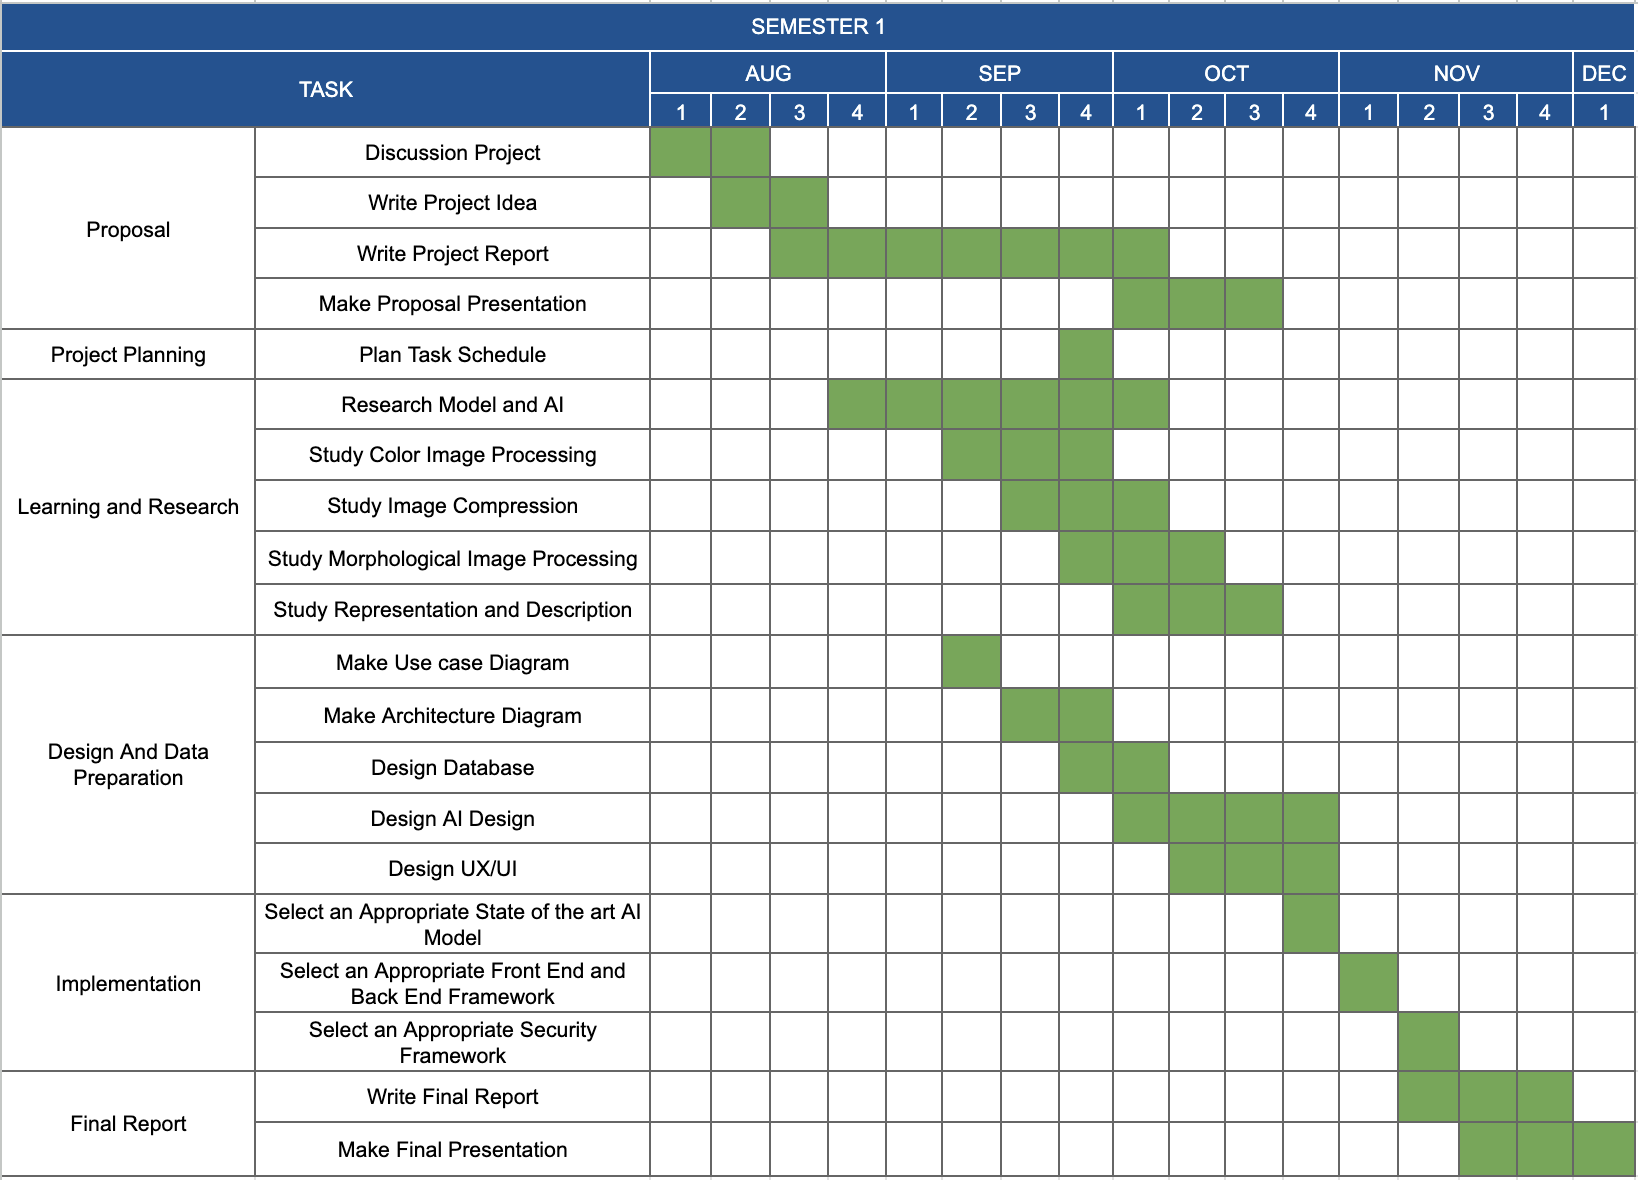
\includegraphics[width=10cm]{./assets/schedule-term1.png}}
\caption{Schedule for first semester}\label{fig:figure-1.1}
\end{figure}

For the second semester, our project focus on implementing the form extractor and generative AI for the process of detect a form. We also focus on web application development and integrate a web application with the form extractor. also including the testing phase a system evaluation.

\begin{figure}[H]
\centering
\fbox{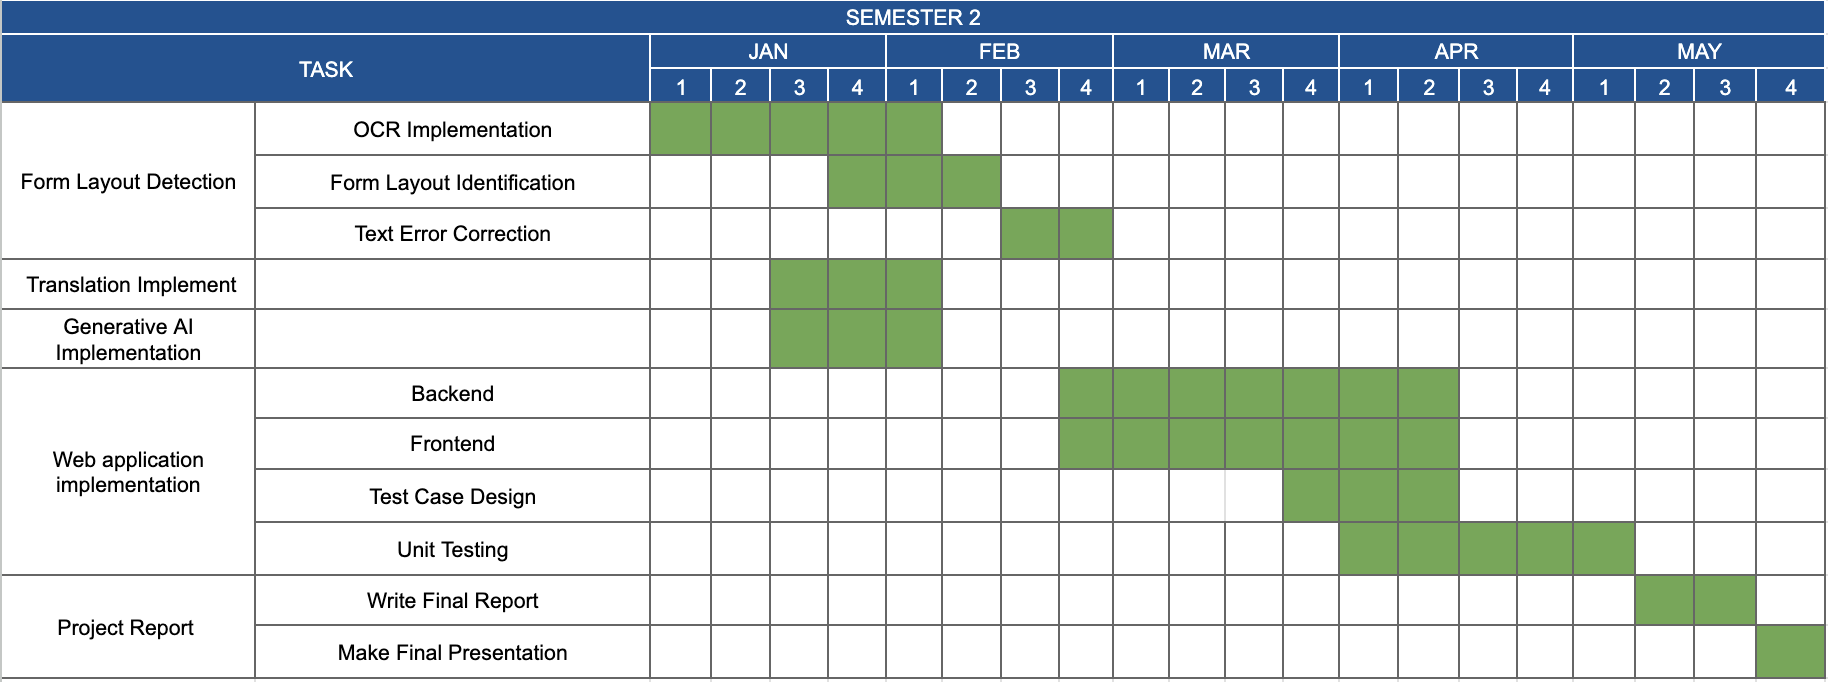
\includegraphics[width=10cm]{./assets/schedule-term2.png}}
\caption{Schedule for second semester}\label{fig:figure-1.2}
\end{figure}

\section{Expected Outcomes}
This project aims to develop a fully functional web application that able to converting a paper-based form or pdf form into a web-based form by utilizing a generative AI for generate a data type of form label. And the web application should reduce a time developer have spend when they converting a form.

%%%%%%%%%%%%%%%%%%%%%%%%%%%%%%%%%%%%%%%%%%%%%%%%%%%%%%%%%%%%
%%%%%%%%%%%%%%  Literature Review %%%%%%%%%%%%%%%%%%%%%%%%%%
%%%%%%%%%%%%%%%%%%%%%%%%%%%%%%%%%%%%%%%%%%%%%%%%%%%%%%%%%%%%
\chapter{Background Theory and Related Research}

\section{Introduction and Background}
\subsection{Introduction}
This chapter will explain the details of the core concept and the solution planning. Theory and core concepts, languages and technologies, and related research will be discussed in this chapter. First, we will cover a core concept of artificial intelligence, machine learning, natural language processing and image processing etc.. Second, the languages and technologies that we interest in the project including a frontend and backend technology. Lastly, related research and competing solutions that are similar to our project will be in research and competing solutions.

\subsection{Background}
The digital transformation of businesses has been accelerated by the need for faster, more reliable ways to handle data. Although many organizations have begun to adopt digital processes, a significant number still rely on paper forms, which can slow down operations and increase the risk of errors. Manual data entry, in particular, is an inefficient method that often leads to mistakes, misinterpretations, and lost time. \par
To solve these problems, many organizations are looking for ways to turn paper forms into digital formats automatically. This is where AI comes in. AI tools can be trained to read forms and convert them into digital versions, speeding up the process and reducing errors. By automating this task, businesses can save time, lower costs, and reduce mistakes, allowing employees to focus on more important tasks.\par
This chapter will explain the main ideas behind the project. It will also discuss the technologies used in the project and look at similar research in the field of form automation.

\section{Theory and Core Concepts}
\subsection{Artificial Intelligence (AI)}
Artificial Intelligence (AI) refers to the study and development of intelligent machines and software that can reason, learn, communicate, and perceive objects, aiming to mimic human-like behavior. Coined by John McCarthy in 1956, AI is a branch of computer science that focuses on enabling computers to perform tasks typically requiring human intelligence, such as problem-solving, perception, and decision-making.

\subsection{Machine Learning (ML)}
Machine Learning is an application of Artificial Intelligence (AI) that provides systems the ability to automatically learn and improve from experience without being explicitly programmed. Machine Learning is crucial in building systems that can automatically learn to recognize patterns and improve over time with more data.

\textbf{Machine Learning Method:}
\begin{itemize}
    \item \textbf{Supervised Learning:} A type of machine learning where the model is trained using a labeled dataset. This means the data comes with answers, so the model learns to make predictions or classify information correctly.
 
    \item \textbf{Unsupervised Learning:} A type of machine learning where the computer learns from data without labels or answers. Instead of being told what to look for, the model tries to find patterns or group similar data points together on its own.
    
    \item \textbf{Semi-supervised learning:} Like a mix of supervised and unsupervised learning. It uses a small amount of labeled data (with answers) and a large amount of unlabeled data (without answers) to train the model. The labeled data helps guide the model, while the unlabeled data helps it find patterns and improve accuracy.
\end{itemize}



\subsection{Natural Language Processing (NLP)} Natural Language Processing (NLP) enables machines to understand, interpret, and generate human language in a valuable way. The process involves several key techniques: Tokenization: Breaking down text into smaller units (tokens), such as words or phrases, which can be analyzed separately. Stop Word Removal: Eliminates common words that provide little informational value, focusing on more meaningful words. Lemmatization and Stemming: Reduces words to their root forms to unify different inflected versions (e.g., "walking" becomes "walk"). Part-of-Speech Tagging: Assigns tags to words based on their grammatical roles (nouns, verbs, adjectives, etc.).

\subsection{Deep Learning} Deep Learning is a type of machine learning where computers are trained to think and learn like humans by processing large amounts of data. It uses a special kind of program called a neural network, which is inspired by the way our brains work. These networks can figure out patterns and make decisions on their own, such as recognizing faces in photos, translating languages, or even predicting what you might want to buy.

\begin{figure}[H]
\centering
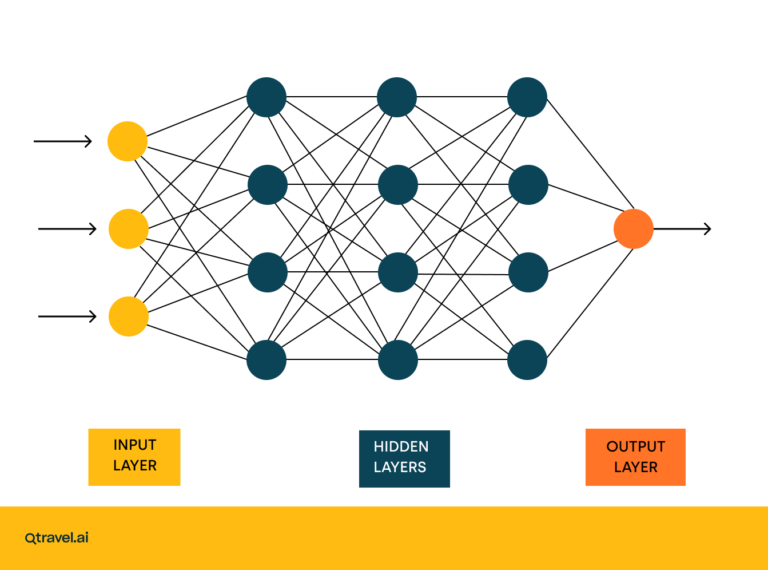
\includegraphics[width=10cm]{./assets/Natural-Network.png}
\label{fig:Natural-Network}
\caption{Natural Network from 
\href{https://www.qtravel.ai/wp-content/uploads/2023/07/sieci-neuronowe-grafika-768x570.png}{Qtravel.ai}.}
\end{figure}

\newpage


\subsection{Generative AI} Generative AI refers to deep learning models that can generate high-quality text, images, and other content based on trained data.  It works by analyzing a lot of data, such as Wikipedia articles or famous paintings, and then using what it learns to produce original outputs similar to the data it studied. \par
In the past, AI models like Variational Autoencoders (VAEs) and Generative Adversarial Networks (GANs) helped create realistic images and sounds. Now, newer models like transformers have taken over. Transformers are powerful because they can learn from massive amounts of text without needing people to label everything.

\subsubsection{Types of Transformer models}
\begin{enumerate}
	\item \textbf{Encoder-only models} (such as BERT): Great for understanding and categorizing text but not for generating new content.
	\item \textbf{Decoder-only models} (such as GPT): Focus on predicting the next word and are good at creating new text.
	\item \textbf{Encoder-decoder models} (such as T5): Combine both approaches and can handle tasks like summarizing or translating text.
\end{enumerate}


\subsection{Portable Document Format.}

The Portable Document Format (PDF) is developed by Adobe in early 1993, it is a file format designed to display documents consistently across device and platform. The strength is preserve the formatting, fonts, images, and layout of the original document, ensuring a consistent and reliable presentation. A PDF file can include a varies type of content, such as text, image, vector graphics, hyperlinks, forms, annotations and even multimedia elements like audio and video.

\subsubsection {PDF Categories}

\begin{enumerate}
	\item \textbf{PDF}: A standard PDF format, It is often used for sharing and viewing files online.
	
	\item \textbf{PDF/A} : For long-term archiving; restricts elements like JavaScript and multimedia.
	
	\item \textbf{PDF/E} : Tailored for engineering, construction, and manufacturing documents.
	
	\item \textbf{PDF/X} : Preferred by print and graphic professionals for consistent visual output.
	
	\item \textbf{PDF/VT} : Like PDF/X but allows variable and transactional printing (customization).
	
	\item \textbf{PDF/UA} : Accessible format supporting assistive technologies for users with disabilities.

	\item \textbf{PAdEs} : Standard for legally binding electronic signatures.

	\item \textbf{PDF Healthcare} : Ensures best practices for healthcare-related data handling.

	\item \textbf{Searchable PDF} : Combines image-based content with searchable text via OCR.

\end{enumerate}

\subsubsection {PDF File Structure}

The PDF file is consists of four part component that describe every pdf file, And all information in pdf is represent in ASCII 

\begin{enumerate}
	\item \textbf{Header}: The first line of the PDF file that specific the version of the PDF.
	\item \textbf{Body} : Contains the document’s main content, including pages, text, and images.
	\item \textbf{Cross-reference table (XRef)} :  Indexes the locations of all objects in the file.
	\item \textbf{Trailer} : Provides structural information and indicates the starting point for reading the document.
\end{enumerate}


\subsection{Text Parser}

Text parsing is the process of analyzing a string of text to extract meaningful information or convert the text into a structured format that a computer program can process. The primary goal of text parsing is to decompose and interpret text data, often transforming unstructured or semi-structured text into a structured form for further analysis or manipulation.

\subsection {No Language Left Behind (NLLB)}

No Language Left Behind (NLLB) is a groundbreaking AI project developed to address the challenge of multilingual translation, particularly for low-resource languages. The project aims to ensure that no language is left behind in digital communication by providing high-quality translation models for over 200 languages, including low-resource languages such as Asturian, Luganda, and Urdu. This initiative promotes linguistic diversity, enabling users around the world to access, share and communicate in their native languages.
At its core, NLLB is a Multilingual Machine Translation (MMT) system that leverages deep learning techniques to train models capable of handling 218 languages across over 40,000 translation directions. The project introduces NLLB-200, a family of models with varying sizes and performance levels, allowing users to select models based on the computational resources available and the accuracy required for their applications.

\subsubsection{Model Architecture and Training}

NLLB-200 is built on the Transformer architecture, a deep learning model that has become the standard in natural language processing tasks.NLLB-200 employs several advanced techniques:

\begin{enumerate}
	\item NLLB-200 uses a special design called a Mixture of Experts (MoE). Instead of using the full model for every input, it turns on just a few parts (called "experts") depending on the input sentence. This makes it possible to build a very large model up to 54 billion parameters without needing huge computing power all the time.
	\item When translating, the model uses special tags to know which language it’s translating from and to. It also uses one big shared list of words (called a vocabulary) across all languages. This helps the model understand patterns between different languages, even ones that are far apart.
	
	\item A good translation model needs high-quality examples. Meta created tools to search and clean up sentence pairs in hundreds of languages. They used techniques like LASER3 (which helps find similar sentences in different languages) and other mining tools to gather the best data possible.
	\item Before training the model to translate, Meta first let it read a huge amount of text in different languages. This helped the model learn how language works in general, even without translations. After that, they fine-tuned it using proper translation pairs..
\end{enumerate}

\newpage

\subsection{Security of Web Form} Web form security is essential as these forms are highly vulnerable to cyberattacks, making them prime targets for malicious parties aiming to access sensitive user data. 
Common threats include:
\begin{enumerate}
	\item \textbf{Cross-Site Scripting (XSS):} Attackers inject malicious scripts into web forms or application code, which can steal user information like keystrokes or cookies, or redirect users to harmful websites.
	\item \textbf{SQL Injection:} Attackers manipulate SQL code within web forms to access or alter databases. This technique can expose or modify sensitive data, and it’s one of the oldest and most dangerous web vulnerabilities.
	\item \textbf{Cross-Site Request Forgery (CSRF):} Attackers trick users into performing unintended actions, such as submitting forms or transferring data, without their knowledge. These attacks exploit the user’s browser and session data.
	\item \textbf{Data Breaches:} A variety of attacks can lead to breaches, exposing sensitive customer information and damaging a business's reputation, as users lose trust in the website's security.
\end{enumerate}

	Many data privacy laws now regulate how web applications must ensure security, especially when handling personal information. The rules we must follow may depend on where our business is located and how it operates. To stay compliant, website owners need to adopt secure practices for web forms.

\textbf{Key laws to be aware of}
\begin{enumerate}
	\item \textbf{GDPR (General Data Protection Regulation)}
	\item \textbf{CCPA, CPRA (California Consumer Privacy Act and California Privacy Rights Act)}
	\item \textbf{HIPAA (Health Insurance Portability and Accountability Act)}
	\item \textbf{PCI DSS (Payment Card Industry Data Security Standard)}
\end{enumerate}

\textbf{Key measures for securing web forms}
\begin{enumerate}
	\item \textbf{Use TLS/SSL Certificates:} TLS/SSL certificates create encrypted links between browsers and servers, ensuring that data transferred is protected. Extended Validation (EV) certificates provide the highest level of security.
	\item \textbf{Encrypt Data:} End-to-end encryption (E2EE) ensures that data is protected throughout its journey from sender to recipient, preventing unauthorized access. Use SSL certificates and CDNs to enhance security.
	\item \textbf{Validate and Sanitize Input:} Validate and sanitize user inputs to prevent attacks like SQL injections or cross-site scripting (XSS). Validation checks if inputs are correct, while sanitization removes harmful data.
	\item \textbf{Collect Minimal Data:} Only collect necessary information to reduce the impact of potential data breaches. This minimizes risk and aligns with privacy regulations like GDPR and CCPA.
	\item \textbf{Anonymize Data:} Mask sensitive data (e.g., credit card numbers) using techniques like asterisks or data shuffling, making it harder for attackers to misuse it.
	\item \textbf{Ask for Consent:} Obtain clear user consent before collecting personal data, and provide easy access to your privacy policy outlining how data is used and protected.
	\item \textbf{Restrict File Uploads:} Limit file uploads by allowing only authorized users, setting file size limits, and using whitelist file types to prevent malware.
	\item \textbf{Use reCAPTCHA:} Implement reCAPTCHA to differentiate between humans and bots, helping reduce spam and prevent automated attacks.
	\item \textbf{Require Authentication:} For sensitive forms, require users to authenticate (e.g., through login or multi-factor authentication) to restrict access to authorized individuals only.
	\item \textbf{Use Virus and Malware Protection:} Employ virus and malware protection through layered security, such as firewalls, malware scans, and intrusion detection, to safeguard your web forms from threats.
\end{enumerate}

\section{Languages and technologies}
\subsection{Web Development Language}
\subsubsection{HTML} HTML (HyperText Markup Language) is the standard language for creating and designing web pages. It is a markup language, which means that specific tags are used to structure web content. Each tag specifies a particular aspect of a website, such as text, photos, links, and multimedia.

\subsubsection{TypeScript} TypeScript is a superset of JavaScript that introduces static typing. It was created by Microsoft to solve some of the limitations of JavaScript, particularly in large-scale applications. Because TypeScript is a superset, it supports all JavaScript features while also adding new functionalities, notably those aimed at increasing code dependability and maintenance.

\subsection{Front-end Technology}
\subsubsection{Vue.js} Vue.js is a JavaScript framework for building user interfaces. It builds on top of standard HTML, CSS, and JavaScript and provides a declarative, component-based programming model that helps you efficiently develop user interfaces of any complexity.

\subsubsection{TailwindCSS} Tailwind CSS is a utility-focused CSS framework that simplifies web development by providing pre-designed utility classes. These utility classes allow you to create custom designs.

\subsubsection{Formkit} Formkit is modern form-building library for Vue.js, designed to help developers create and manage forms with minimal effort and maximum flexibility.

\subsection{Backend Technology}
\subsubsection{FastAPI} FastAPI is a modern web framework for creating Python APIs that prioritizes speed, ease of development, and automated validation. It has gained popularity for developing quick, high-performance APIs because it uses Python type hints to provide explicit, automatic data validation and interactive API documentation.

\subsubsection{Pydantic} Pydantic is a Python data validation and parsing library that enforces data types and restrictions using Python type annotations. Although it can be used separately, it is an essential part of FastAPI. With Pydantic models, you can easily serialize data, validate incoming data, and specify the structure of your data.

\subsubsection{SQLModel} SQLModel is the Python SQL toolkit and Object Relational Mapper that gives application developers the full power and flexibility of SQL without creating a SQL statement.

\subsubsection{PostgresSQL} The PostgreSQL popular open-source relational database management system (RDBMS) for managing and storing data. It is renowned for being reliable, effective, and compliant with SQL standards. And It support storing a json format data type which it can be act as NoSQL in some situation.

\subsection{Document Processing}
\subsubsection{Python} Python Programming language is a popular high-level computer programming language for machine learning because it is simple to use and easy to read and write. Additionally, it has a fast processing speed. Web development, data analysis, automation, scientific computing, and many more topics are among the many libraries available.

\subsubsection{PyMuPDF} PyMuPDF is a A powerful Python package for extracting, analyzing, converting, and manipulating data from PDF documents.

\subsubsection{NLLB-200} NLLB-200 (No Language Left Behind) is a project by Meta (Facebook) that focuses on creating AI models capable of translating between 200 languages.

\subsubsection{PyTorch} PyTorch is an open-source deep learning framework developed by Facebook's AI Research lab (FAIR). It provides tools for building and training neural networks using dynamic computational graphs, which allow for flexibility and ease in model building.

\subsubsection{LLAMA} LLama (short for Large Language Model Architecture) is a type of AI model designed to understand and generate human-like text. It is built using a transformer architecture, which helps it learn language patterns and produce meaningful responses based on its training data.

\section{Competing solutions}
\subsection{Microsoft Azure Document Intelligence}
\begin{figure}[H]
\centering

\includegraphics[width=10cm]{./assets/Microsoft-Azure.jpg}
\caption{Microsoft Azure Document Intelligence from 
\href{https://learn.microsoft.com/th-th/training/achievements/extract-data-from-forms-use-form-recognizer.svg}{Learn.microsoft.com}.}
\label{fig:microsoft-azure-doc}  
\end{figure}

	Microsoft Azure Document Intelligence is a solution that provides a feature of capturing data from printed or handwritten forms. And create a flow pipeline with Azure Cognitive Search pipeline to complete workflow as the user needs.
	
%%%%%%%%%%%%%%%%%%%%%%%%%%%%%%%%%%%%%%%%%%%%%%%%%%%%%55
%%%%%%%%%%%%%%%%%%%%%%%%%%%%%%%%%%%%%%%%%%%%%%%%%%%%%
%%%%%%%%%%%%%%CHAPTER 3 DESIGN AND METHODOLOGY%%%%%%%%%%%%%%%%
%%%%%%%%%%%%%%%%%%%%%%%%%%%%%%%%%%%%%%%%%%%%%%%%%%%%%
\chapter{DESIGN AND METHODOLOGY}

This chapter will cover the features, architecture, functionalities, design methods, and
diagrams of our web application. We will delve into the details of the application’s
functionality and architecture.

\section{Project Functionality}

\subsection{System Requirements}

\begin{itemize}
 \item The web application must allow users to log in with email and password. 
 \item The web application must allow the user to upload a form file to the system.
 \item The web application must allow users to fill the form without login.
 \item The web application must allow users to view the data of the form.
 \item The web application must allow users to edit the form before publishing.
 \item The web application must allow users to delete the form.
 \item The web applications must provide the option for all logged-in users to logout.
\end{itemize}

\subsection{Feature List}

\subsubsection{Form Layout Analysis System}

The Form Layout Analysis System will extract all the text from the document that is uploaded by the user via a web application. The system will then analyze the form’s pattern, extract the input labels, translate the text into English, and send the translated information to a generative AI for data type generation.

\subsubsection{Form Schema generator System}

The Form Schema generator System will receive information from the Paper-Based Form Analysis System and Form Schema generator System must be able to generate a form schema that compatible with a form library.

\subsubsection{Web Form System}

The Web Form System must enable users to complete the form, store the data in the database, and see the data created by the form owner.

\subsubsection{Registration and Authentication System}

The Registration and Authentication System must enable a user to register and login to the system by using only email and password. This including a forgot password and the  OTP for reset password.

\section{Use Case Diagram}

From the figure \ref{fig:use-case} The diagram shows a relationship between the user and the system by using a use case diagram. The user of the system is a developer that needs to transform a paper-base form into web application form and the user who going to fill the form. The system consists of 3 different systems, which are form layout analysis system, form schema generator systems, web form systems and registration and authentication systems. The user can upload a paper-based form to the system, and the system will transform the form into a web-based form.

\begin{figure}[!h]
\centering
\fbox{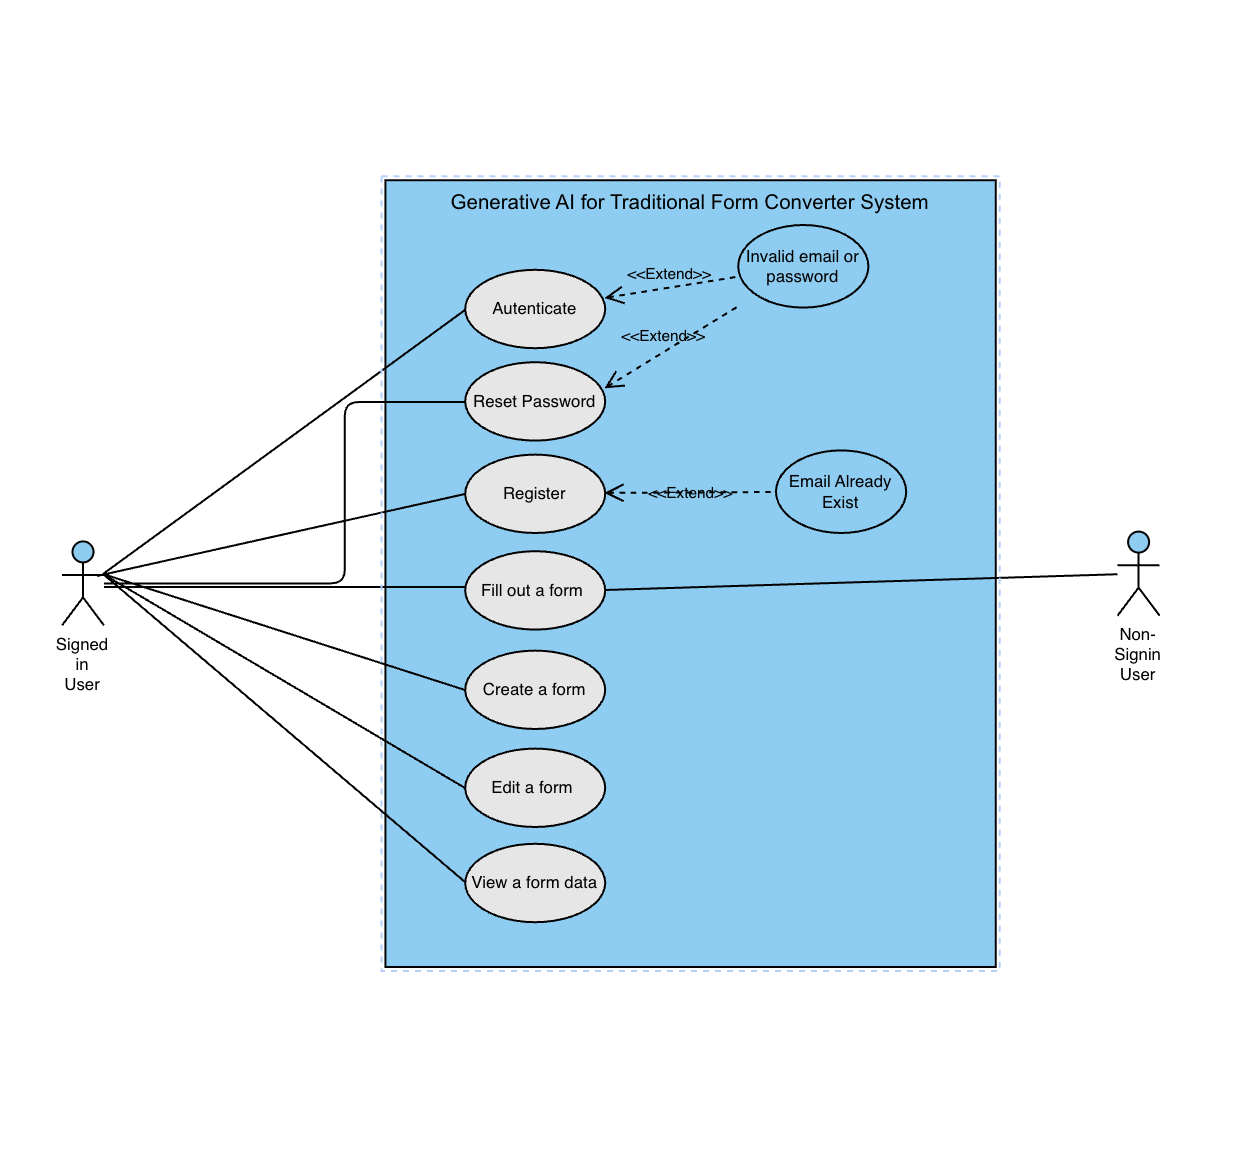
\includegraphics[width=10cm]{./assets/usecase.png}}
\caption{Use case diagram}\label{fig:use-case}
\end{figure}

\section{Use Case Narrative}

\subsection{Autentication}

\noindent\textbf{Use Case Name:} Autentication \\
\textbf{Actors:} Form Creator and Required Login User \\
\textbf{Goal:} Users log in to the system. \\
\textbf{Preconditions:} User is registered

Main Success Scenario: 

\begin{enumerate}
    \item User access the website.
    \item User enter a email and password.
    \item User submit a email and password.
    \item System authenticate and navigate to the home page.
\end{enumerate}

\newpage

\subsection{Register}

\noindent\textbf{Use Case Name:} Register \\
\textbf{Actors:} Form Creator and Required Login User \\
\textbf{Goal:} Users register to a system. \\
\textbf{Preconditions:} User does not have an account

Main Success Scenario: 

\begin{enumerate}
    \item User access the website.
    \item User click to create a new account.
    \item User enter an email and password and personal information.
    \item User submit information.
    \item System saves user information and navigates users to the login page.

\end{enumerate}

\subsection{Create a form}

\noindent\textbf{Use Case Name:} Create a form \\
\textbf{Actors:} Form Creator\\
\textbf{Goal:} Create a form by upload the form file. \\
\textbf{Preconditions:} User has logged in.

Main Success Scenario: 

\begin{enumerate}
    \item User go to home page.
    \item User click at upload a form.
    \item User select a file to upload.
    \item System will process the file and navigate users to the edit form page to confirm a form before publishing.
   
\end{enumerate}

\subsection{Edit a form}

\noindent\textbf{Use Case Name:} Edit a form \\
\textbf{Actors:} Form Creator\\
\textbf{Goal:} Edit a form to make a change.\\
\textbf{Preconditions:} User has logged in.

Main Success Scenario: 

\begin{enumerate}
    \item User go to home page.
    \item User click at edit a form at the form user need to make change.
    \item User make change a form.
    \item User click back to the previous page.
    \item System will process autosave and navigate users to the previous page.
\end{enumerate}


\subsection{View a form data}

\noindent\textbf{Use Case Name:} View a form data \\
\textbf{Actors:} Form Creator\\
\textbf{Goal:}View the data that user have input\\
\textbf{Preconditions:} User has logged in.

Main Success Scenario: 

\begin{enumerate}
    \item User go to home page.
    \item User click at view a data of the form.
    \item User can view a form result.
\end{enumerate}

\subsection{Fill up the form}

\noindent\textbf{Use Case Name:} Fill up the form \\
\textbf{Actors:} Required Login Users and Anonymous User \\
\textbf{Goal:} Add a new data to the form \\
\textbf{Preconditions:} User has logged in or non-login user.

Main Success Scenario: 

\begin{enumerate}
    \item User access a form via the public link
    \item User fill up a form.
    \item User submit a form data.
    \item System will save the data and navigate to the form page again.
\end{enumerate}

Alternate scenario (user access the form required a login without login):

\begin{enumerate}
    \item User access a form via the public link
    \item System will navigate to the login page After login completes the user will redirect back to the form page.
\end{enumerate}

\newpage

\section{Activity Diagram}

From Figure \ref{fig:activity-diagram} The Activity diagram shows the sequence how Generative AI for
Traditional Form Converter System is working.

\begin{figure}[!h]
\centering
\fbox{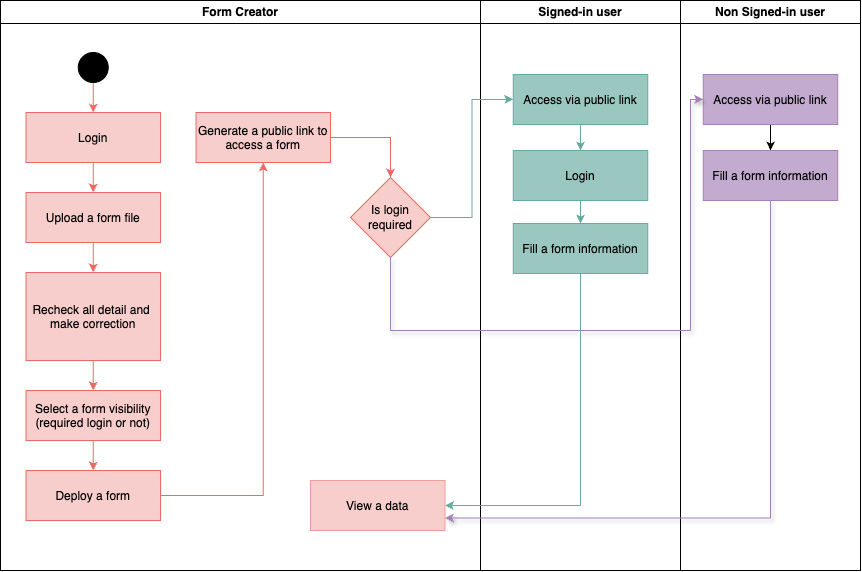
\includegraphics[width=10cm]{./assets/activity-diagram.png}}
\caption{Activity Diagram}\label{fig:activity-diagram}
\end{figure}

\subsection{Form creator}

\begin{itemize}
\item  \textbf{Login:} Form Creator must login before use the system
\item  \textbf{Upload a form file:} After logging in, Form creator must upload a form file to add new form to the system.
\item  \textbf{Recheck all detail and make correction:} In this step, Form creator must check all the information that system has generated and make a correction if incase of error text found.
\item  \textbf{Select a from visibility:} Select a form visibility, whether the form creator need to form to be access by the user who signed-in or anyone can access.
\item  \textbf{Deploy a form and Generate a access link:} In this step, the form will be saved and generated a access link to allow user to access.

\end{itemize}


\subsection{Signed-in user}

\begin{itemize}
\item  \textbf{Login:} If the form requires login, the user must log into the system.
\item  \textbf{Fill out information:} Once logged in, the user going to fills out the form and submit.
\end{itemize}


\subsection{Non Signed-in user}

\begin{itemize}
\item  \textbf{Fill out information:} If login is not required, the user can directly fill out the form without logging in.
\end{itemize}

\newpage

\section{System Architecture}

\begin{figure}[!h]
\centering
\fbox{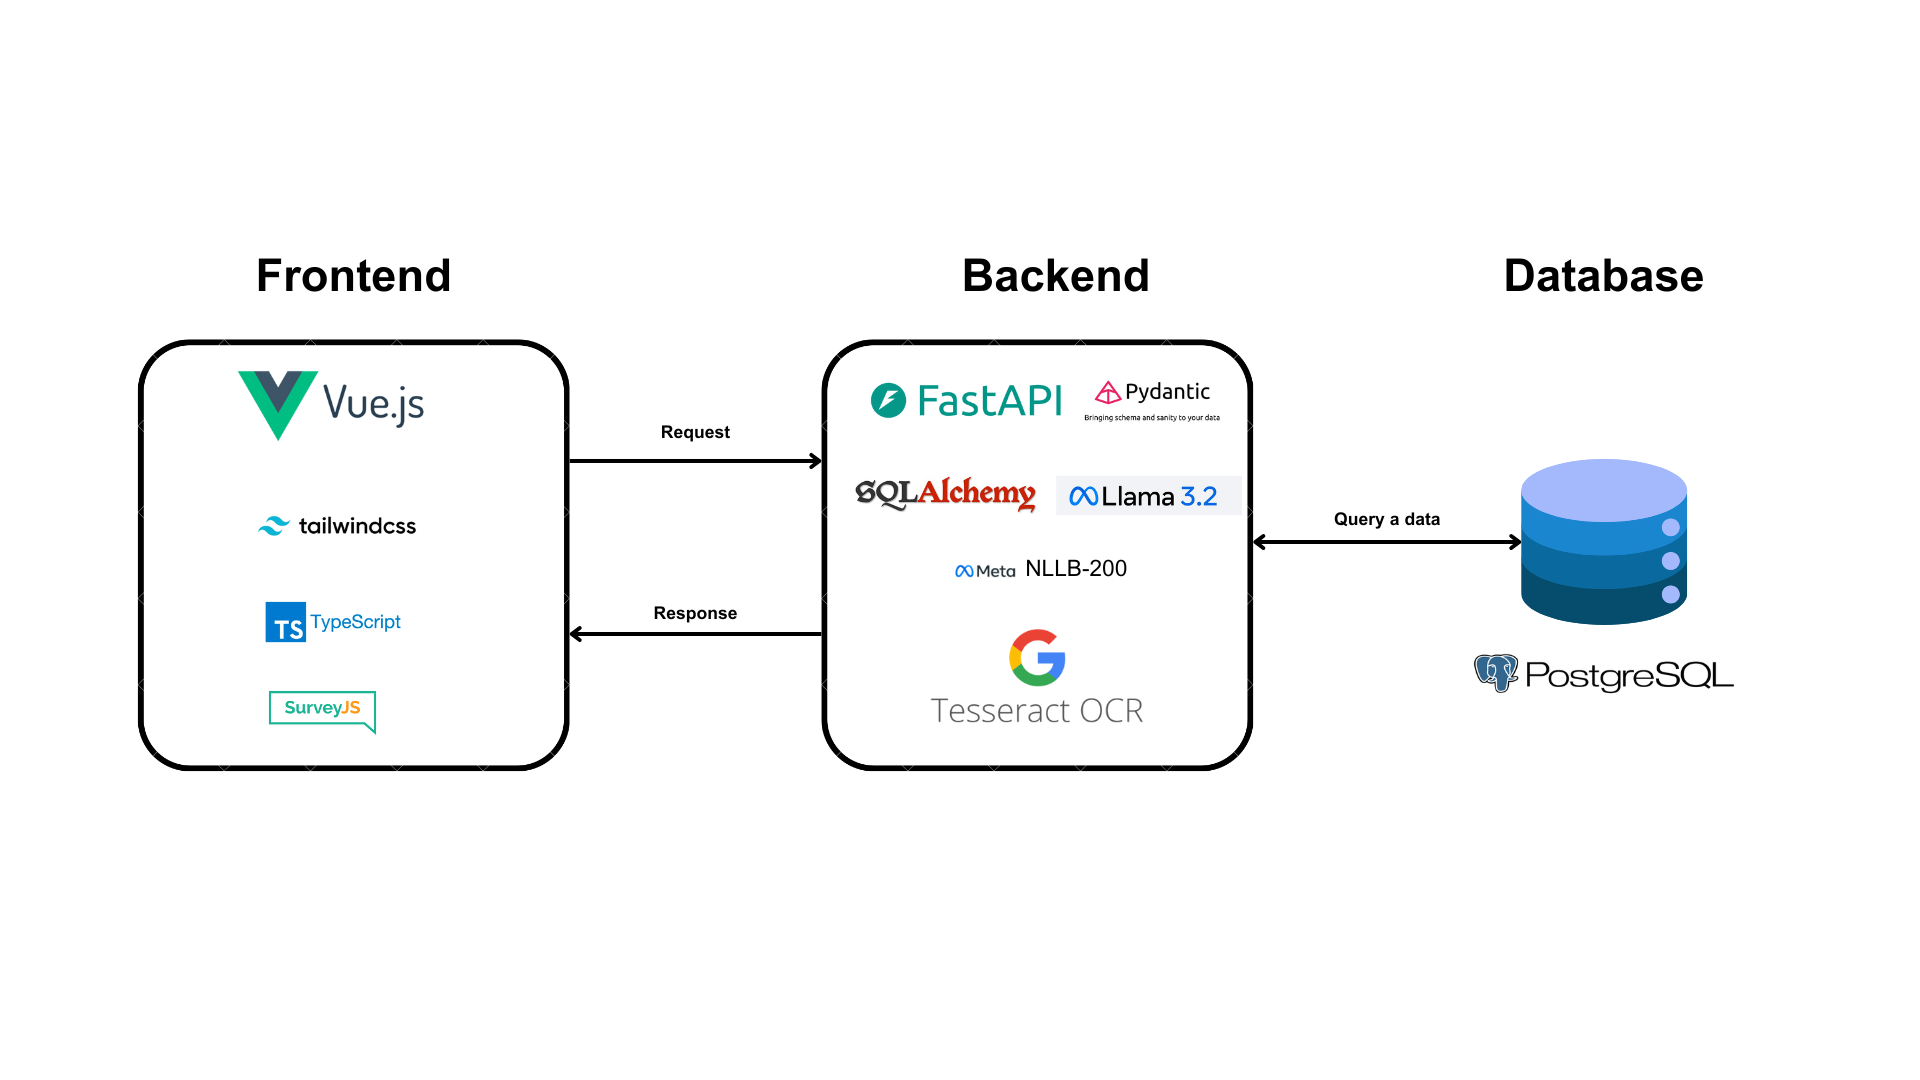
\includegraphics[width=10cm]{./assets/system-arch.png}}
\caption{System Architecture}\label{fig:system-arch}
\end{figure}

Figure \ref{fig:system-arch}, The diagram shown a system architecture in figure above, The System have divided into 3 part which front-end, back-end and database, each part have shown a technology stack, and here are the description of each component

\begin{itemize}
\item  \textbf{VueJS} is a Front-end JavaScript library for building UI
\item \textbf{TailwindCSS} is a CSS framework for styling the UI and used with React
\item \textbf{FastAPI} is a Back-end framework for building REST API
\item \textbf{PostgreSQL}  is a relational database
\item \textbf{Pydantic}  is a python library used for data validation 
\item \textbf{SQLModel} is a Python base Object Relational Mapper (ORM) and SQL Tool kit
\item \textbf{Formkit} is a form engine library for vue.js
\item \textbf{Meta NLLB-200} is a Model for text translation
\item \textbf{PyMuPDF}  is a high-performance Python library for data extraction, analysis, conversion and manipulation of PDF documents.
\item \textbf{Llama 3:8b} is a generative AI from Facebook
\end{itemize}


\section{System Worflow}

\subsection{Extracting text and text parse}

\subsubsection{Extracting text}

Text extraction is the first step after a user uploads a file through the web application. In this stage, a PDF library such as PyMuPDF or pdfplumber is used to extract both the text and layout from the PDF. This is followed by text preprocessing to prepare the content for analysis such as normalizing special dot characters to standard dots to ensure accurate parsing during the next phase.

\subsubsection{Text Parse}

Text parsing is the second process after the extracted text has been completed. Text parse is the process of analyzing a text and breaking down the text to convert it into a structured format, In this process, the purpose of text parse is to analyze the layout of the form, by using a text from a previous process to identify where which text is the label of the input field. The text parse algorithm starts by separating the text from each line and analyzing it line by line, If there is a word in front of the small point the text parse will mark the text as an input label, but if the line starts with the small point the parse will look back to the previous line to check whether if there any text that matches with the condition that parse has.

%\subsubsection{Text Error Correction}

%Text Error Correction is the third process after extracting text and text parse, respectively. Text error correction is identifying and fixing errors in a given text. Text error correction includes spelling mistakes, grammatical errors, punctuation issues, and incorrect word usage. In this process, the text error correction focuses on spelling mistakes and vowel missed order, To make a correction, the first step is to tokenize the whole word into a single word and check the word with a dictionary, If the word does not exist then the system will mark it as an error like this "<ERROR>Wolrd</ERROR>". The system will correct the word with a cosine similarity technique, the technique will convert a dictionary into a vector and also an error text. It will rank with cosine similarity, then it will take the first rank to replace a text. This process is required only for the user who uploads an image.

\subsection{AI Model}

\subsubsection{Translation}

Translation is the fourth process and the first process that AI have involve in the project. Translation is the process of  translate a Thai text to English text by using No Language Left Behind (NLLB) from meta, which the model is aim for high-quality translations directly between 200 languages. And we have selected a fine-tuned version of NLLB, which is wtarit/nllb-600M-th-en model and use it via hugging face transformer.

\subsubsection{Data Type Generator}

The Data Type Generator is the fifth process after preparing the process before the data type generator. The Data type generator is designed to generate a suitable datatype of each input field, for example, birthdate must be Date instead of string, passport number must be string, or text instead of number. All of these types will be applied with the form schema to make a form able to validate a correct data input. The data type generator is going to use a Llama 3 for prompt and generate a schema, and it will use an ollama as an interface for connecting to and communicating with the Llama 3 local model.

\subsection{Form Schema Generator}

The Form Schema Generator is the last process of the flow, the form schema generator will be used to generate a form schema from the output received from the data type generator to show output on the webpage and interact with the user.

\begin{figure}[!h]
\centering
\fbox{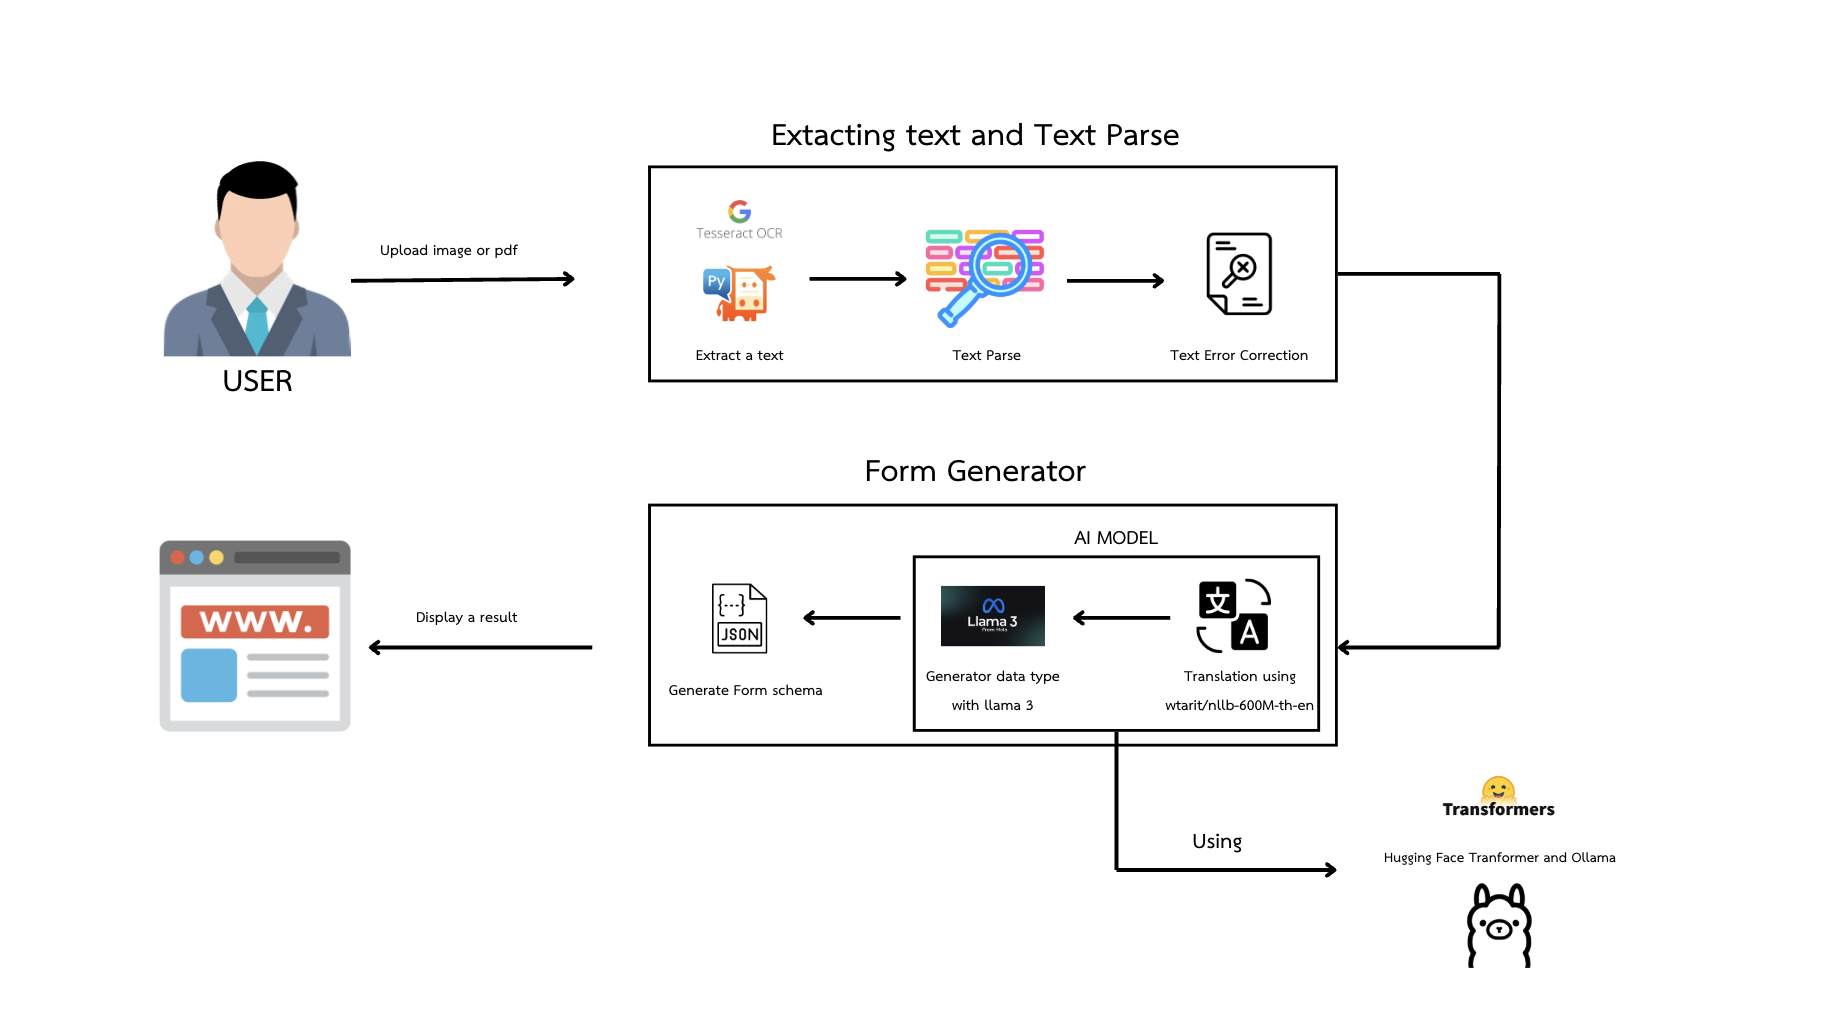
\includegraphics[width=10cm]{./assets/system-flow.png}}
\caption{System Workflow Diagram}\label{fig:system-workflow}
\end{figure}

\newpage

\section{Database Design}

Figure \ref{fig:er-diagram} shown a project database design, the system consist three tables in our project database design are user, form, and form result. table is used to store user data, form result is used to store a result that the user has filled out, and form table is used to store a form schema also a OTP and reset password session table.

\begin{figure}[!h]
\centering
\fbox{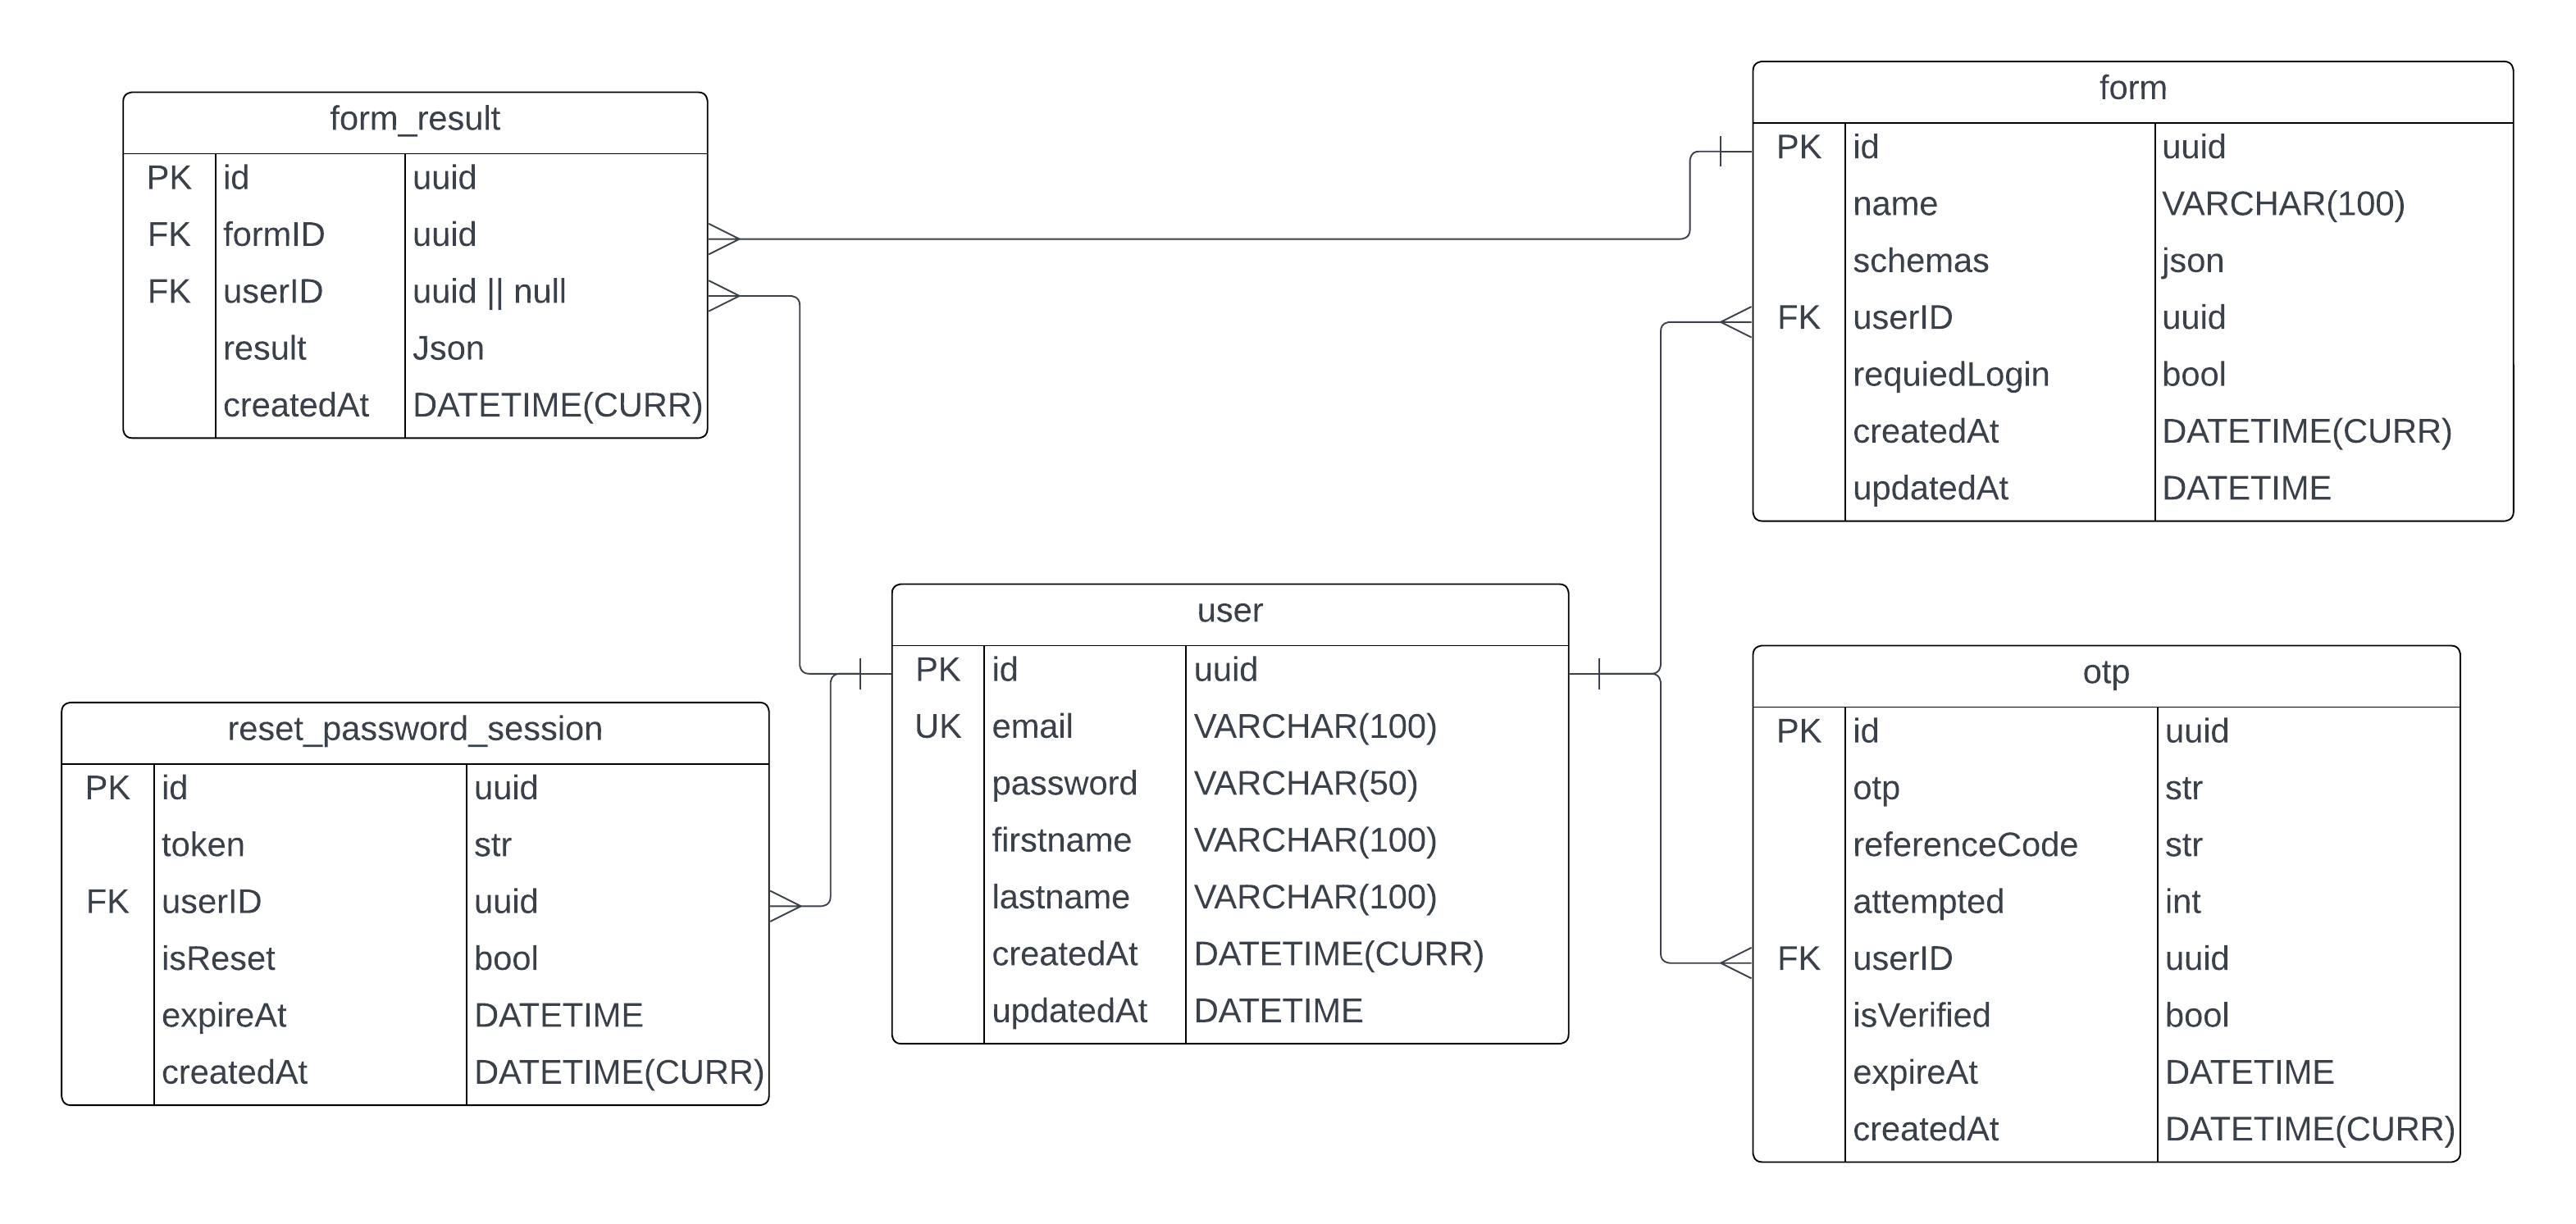
\includegraphics[width=10cm]{./assets/ER-diagram-new.png}}
\caption{ER Diagram}\label{fig:er-diagram}
\end{figure}


\newpage
\section{User Interface Design}

\subsection{Login Page}

\begin{figure}[!h]
\centering
\fbox{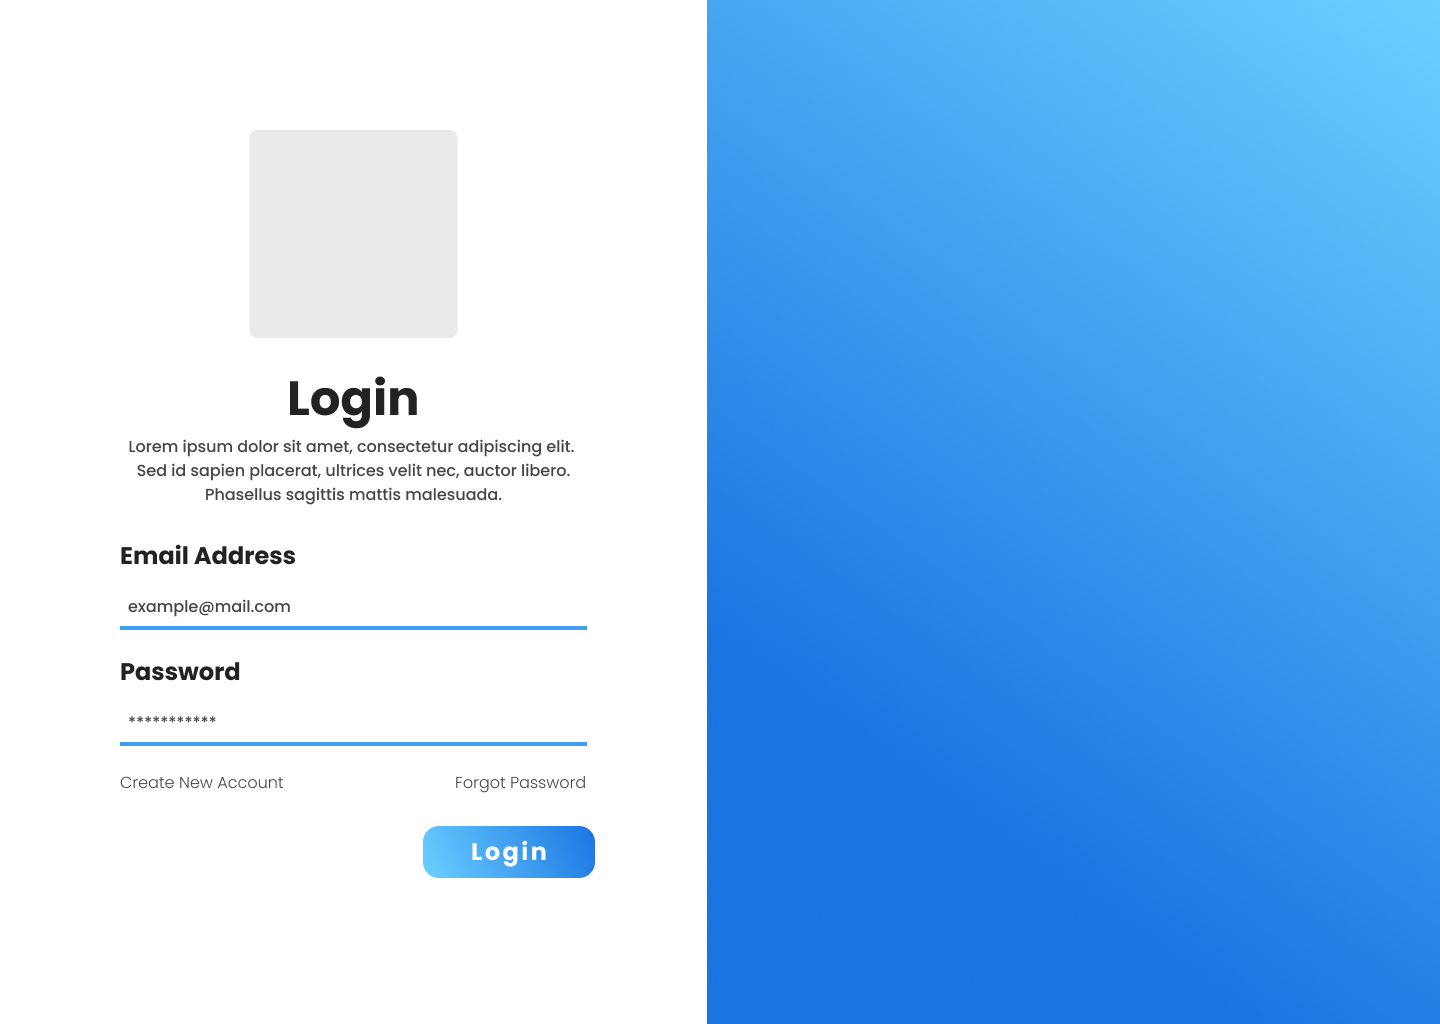
\includegraphics[width= 10cm]{./assets/UI/Login.png}}
\caption{Login Page}\label{fig:login}
\end{figure}

Figure \ref{fig:login} represents the login screen of the web application. This page have a email field,  password field and a login button to sent a credential to the back-end system. 

\subsection{Create Your Account }

\begin{figure}[!h]
\centering
\fbox{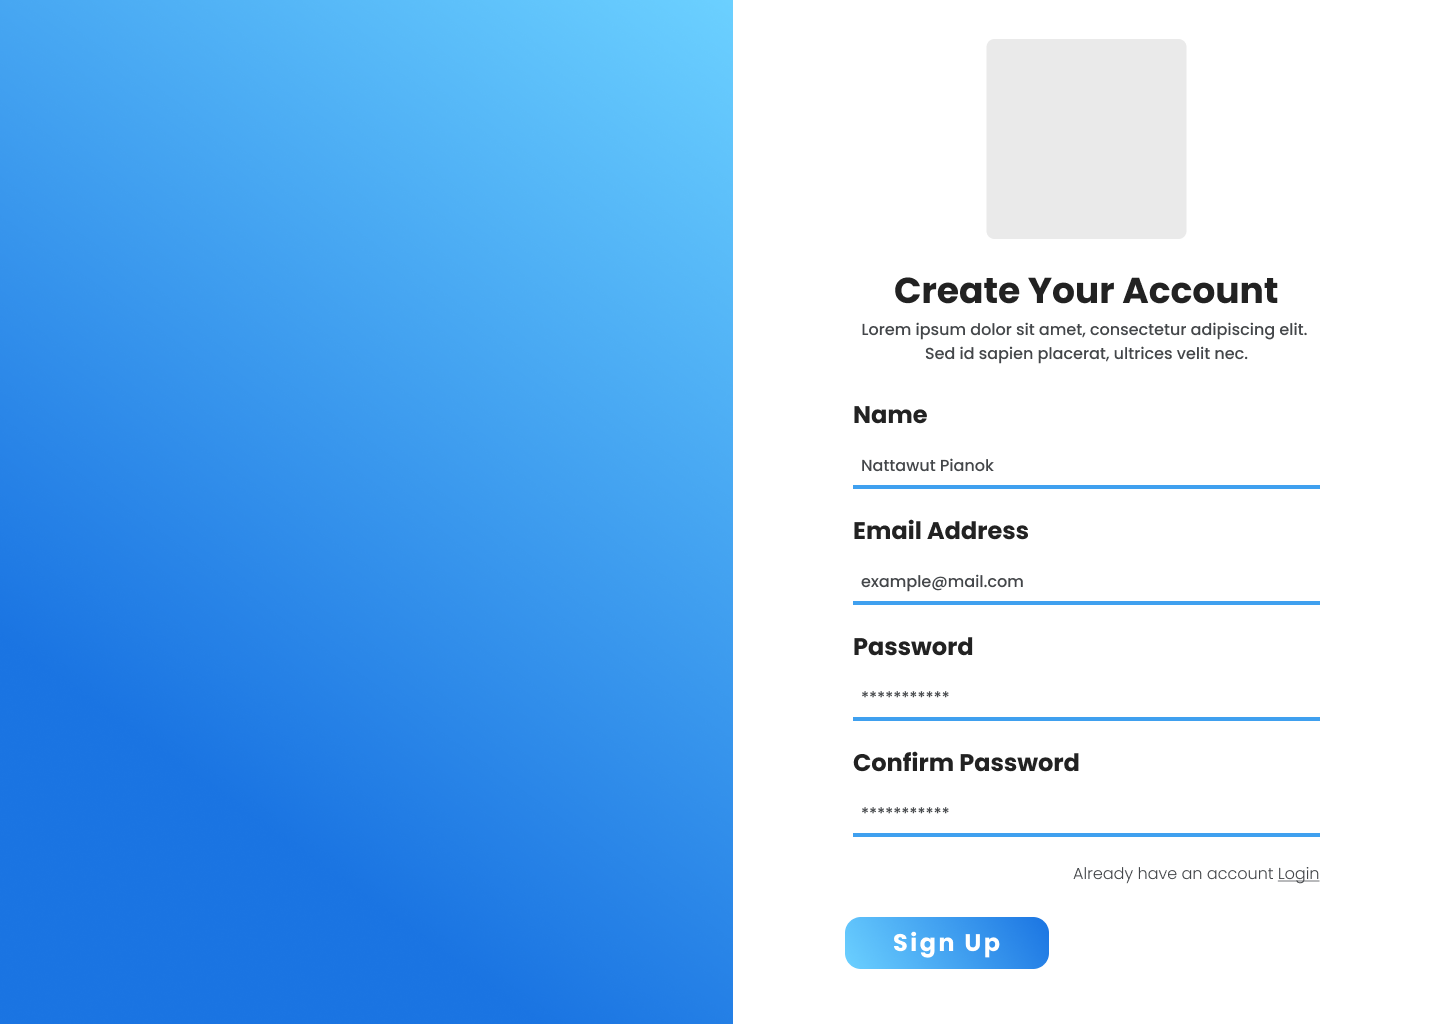
\includegraphics[width= 10cm]{./assets/UI/Sign-Up.png}}
\caption{Create Account Page}\label{fig:create-acc}
\end{figure}

Figure \ref{fig:create-acc} represents the create account page of the web application. This page allow user to create their own account by the user must provide a following field which is name, email and password.

\subsection{Edit Profile}

\begin{figure}[!h]
\centering
\fbox{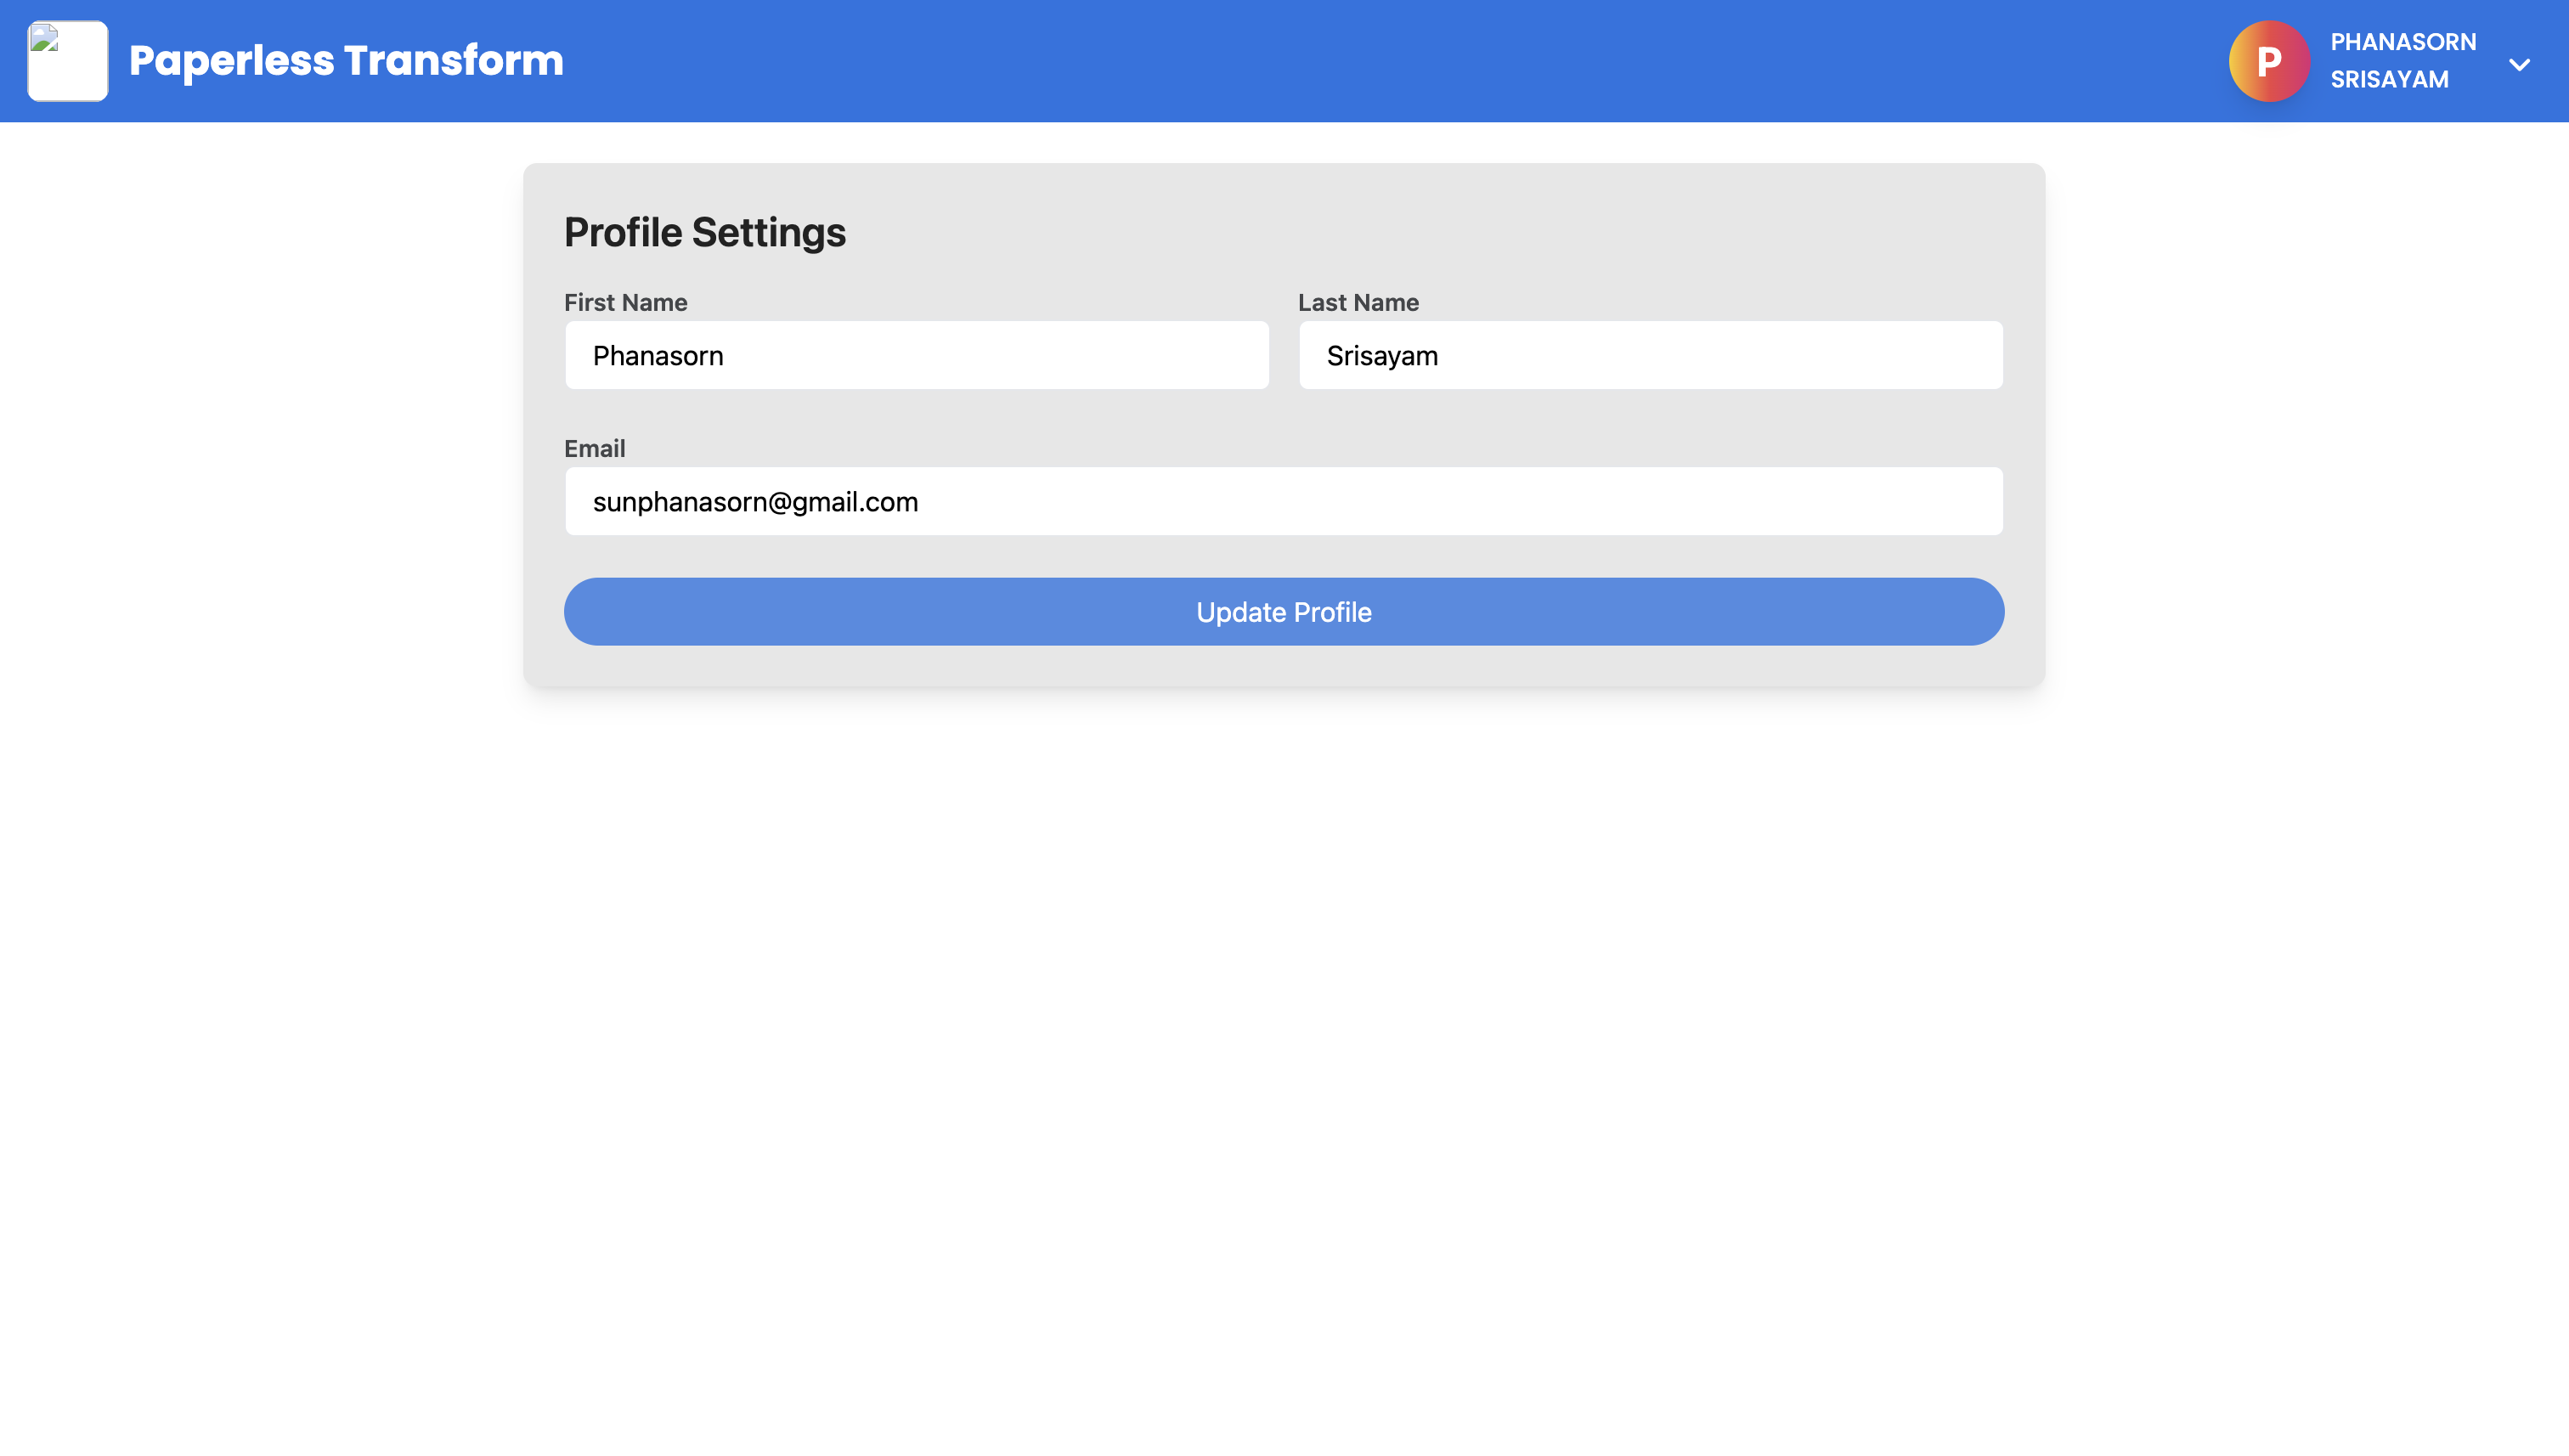
\includegraphics[width= 10cm]{./assets/UI/edit-profile.png}}
\caption{Edit Profile Page}\label{fig:edit-profile}
\end{figure}

Figure \ref{fig:edit-profile} represents the edit profile page of the web application. This page allow user to update their user profile
by user can edit firstname, lastname and email.

\subsection{Forgot Password}

At Figure \ref{fig:Forgot-Password} represents the create account page of the web application. When the user forgot their password, The user must navigate to this page by click at forget password from login page. And fill the email address to allow the system sent the One-time password (OTP) to email address. 


\begin{figure}[!h]
\centering
\fbox{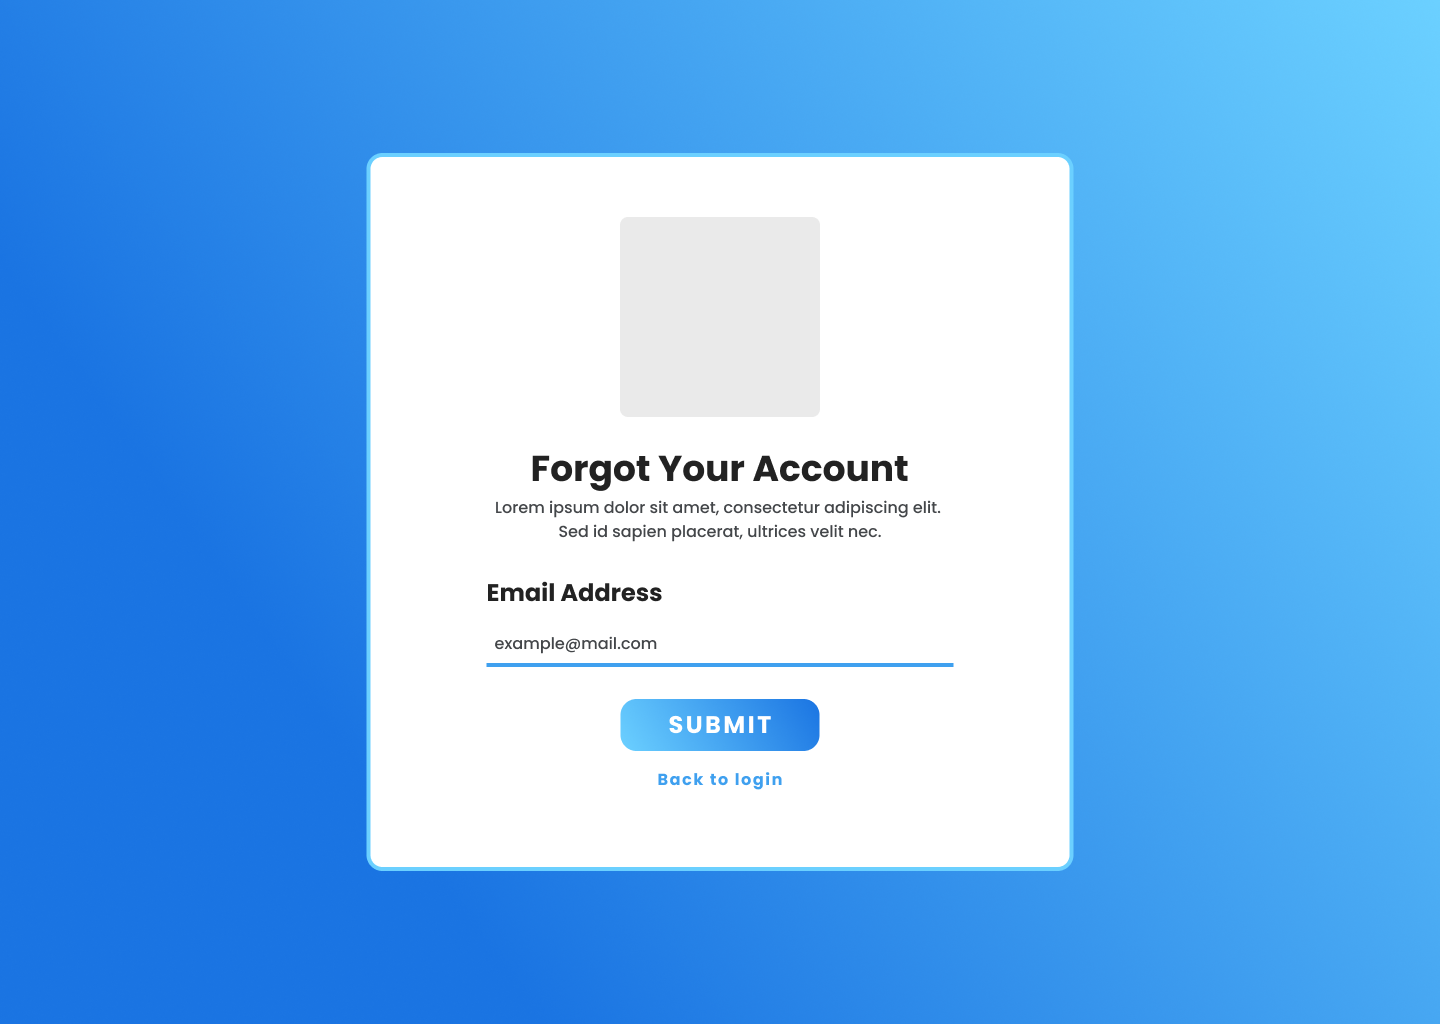
\includegraphics[width= 10cm]{./assets/UI/forgot-password.png}}
\caption{Forgot Password Page}\label{fig:Forgot-Password}
\end{figure}



\begin{figure}[!h]
\centering
\fbox{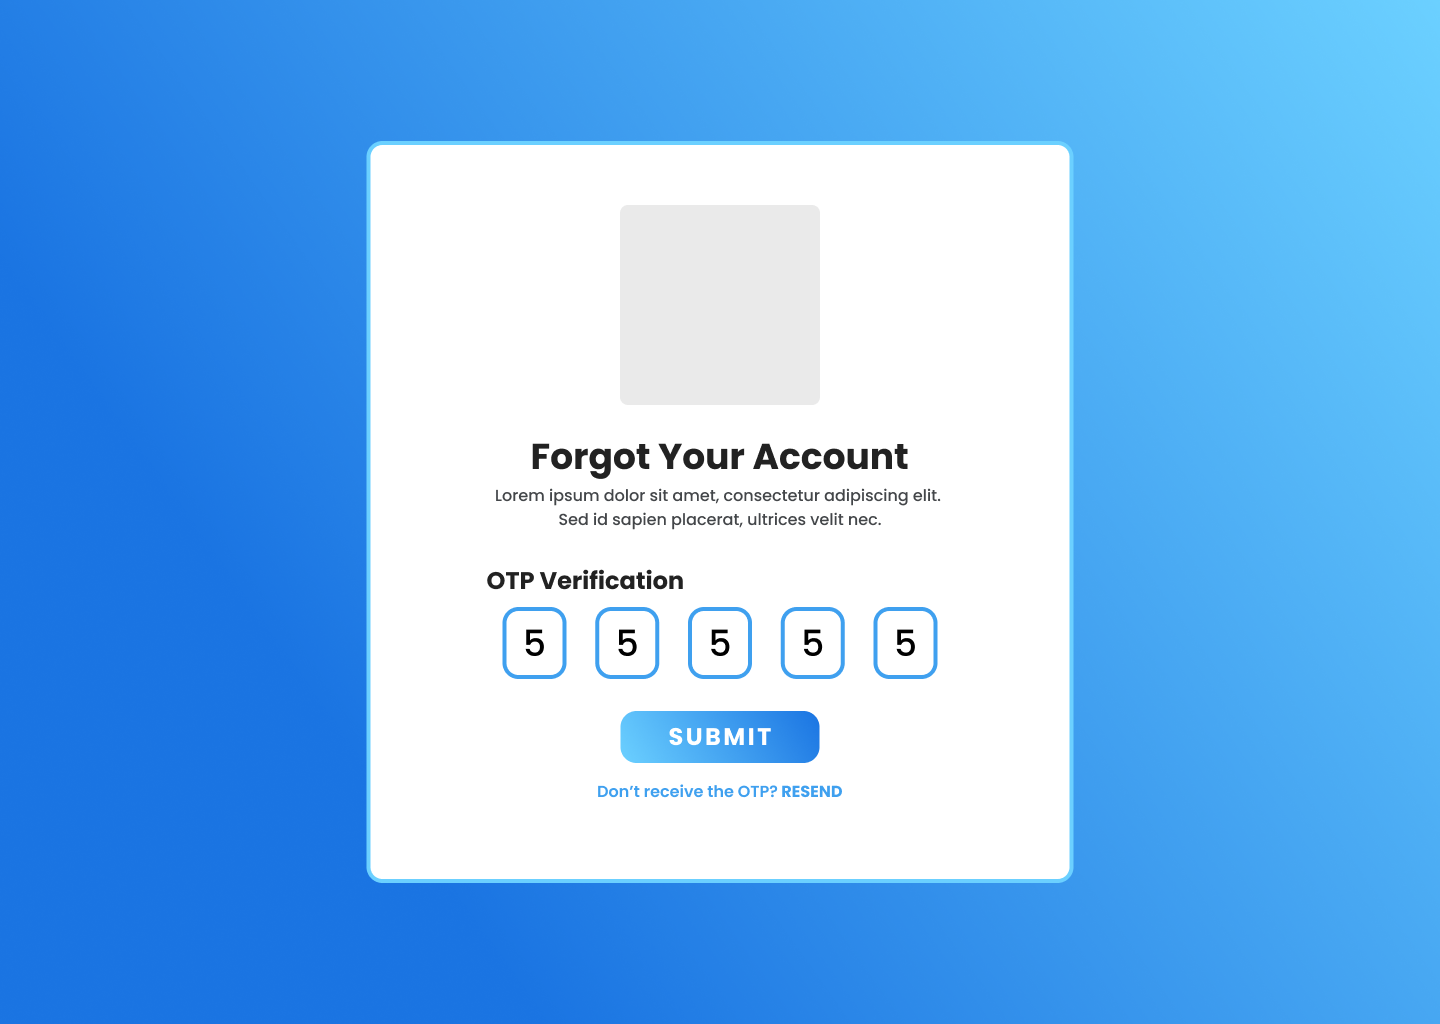
\includegraphics[width= 10cm]{./assets/UI/Forgot-Password-Code.png}}
\caption{Forgot Password Page}\label{fig:Forgot-Password-code}
\end{figure}

\begin{figure}[!h]
\centering
\fbox{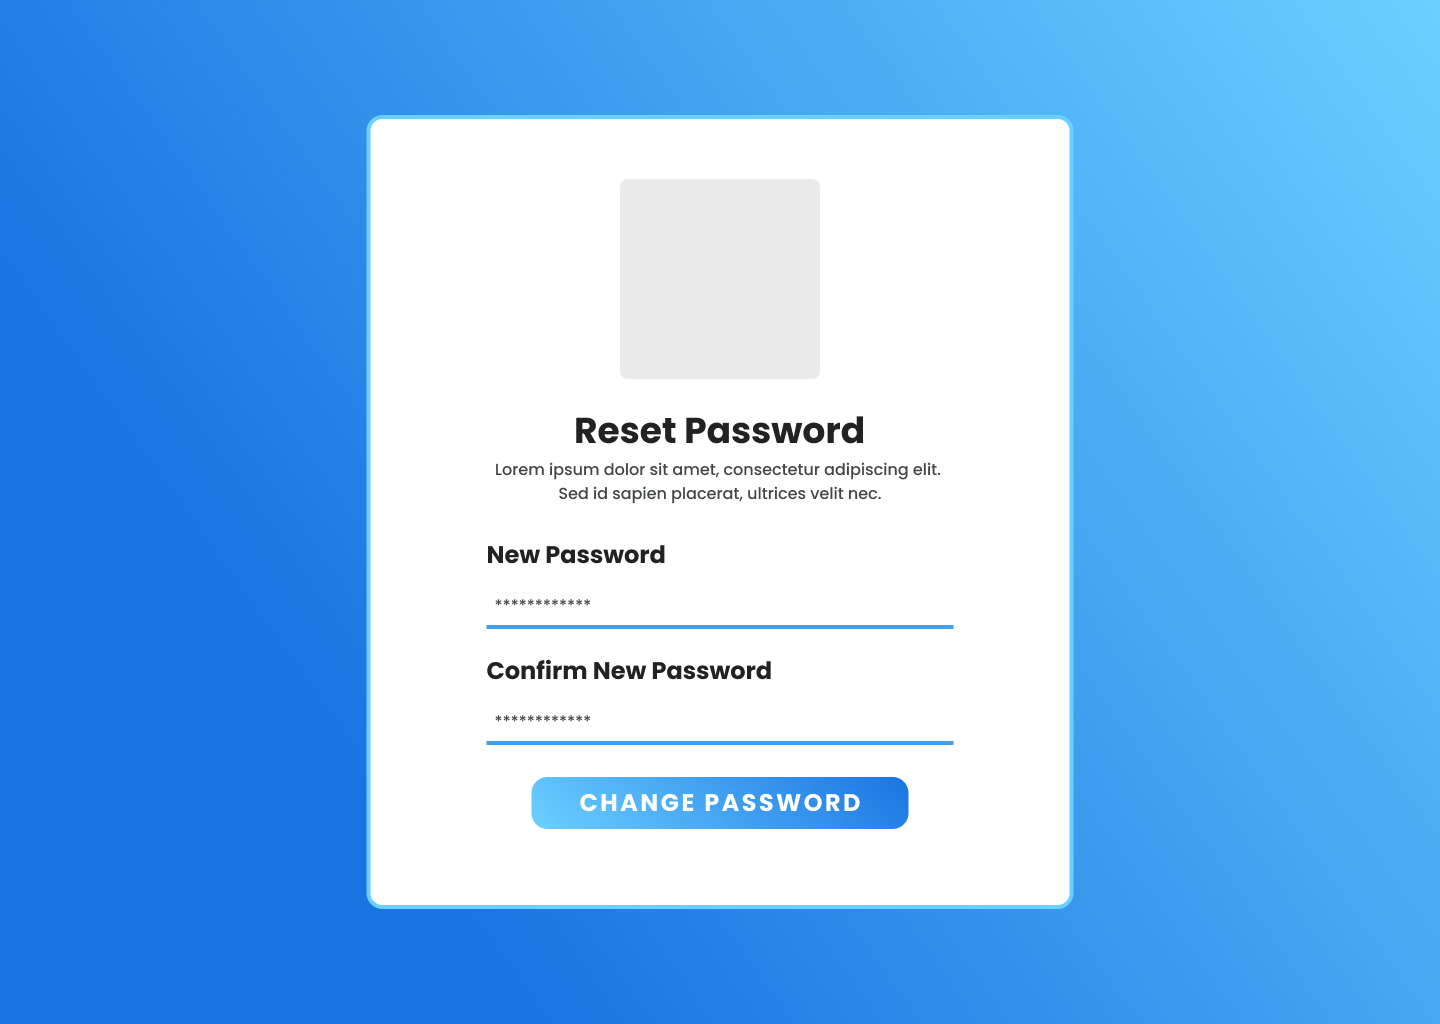
\includegraphics[width= 10cm]{./assets/UI/Reset-password.png}}
\caption{Reset Password Page}\label{fig:Reset Password}
\end{figure}

At the Figure \ref{fig:Forgot-Password-code}, It represents a OTP confirmation page which required a OTP Code that the system have send to the email address. Figure \ref{fig:Reset Password}, It represents a reset password pageIf it success the system will navigate to reset password page for enter a new password.

\newpage
\subsection{Dashboard}

\begin{figure}[!h]
\centering
\fbox{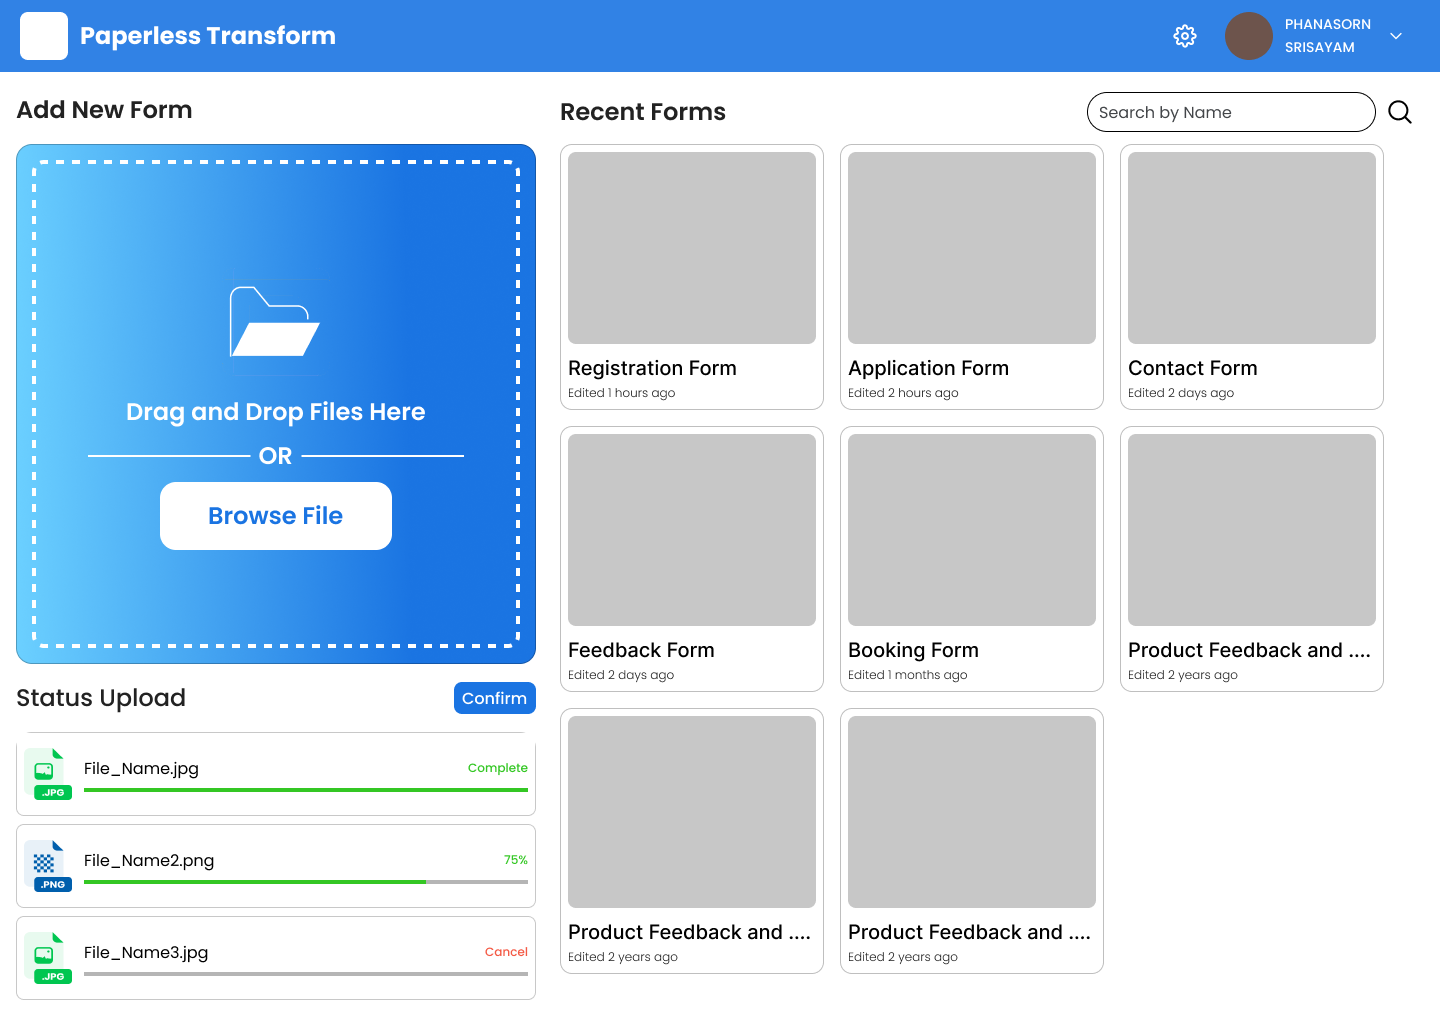
\includegraphics[width= 10cm]{./assets/UI/DashBoard.png}}
\caption{Dashboard Page}\label{fig:Dashboard}
\end{figure}

Figure \ref{fig:Dashboard} represents the dashboard page, it will show all the form that user have and the add form section at the left hand side, also have a upload status while file is uploading.

\newpage
\subsection{Edit Form}

\begin{figure}[!h]
\centering
\fbox{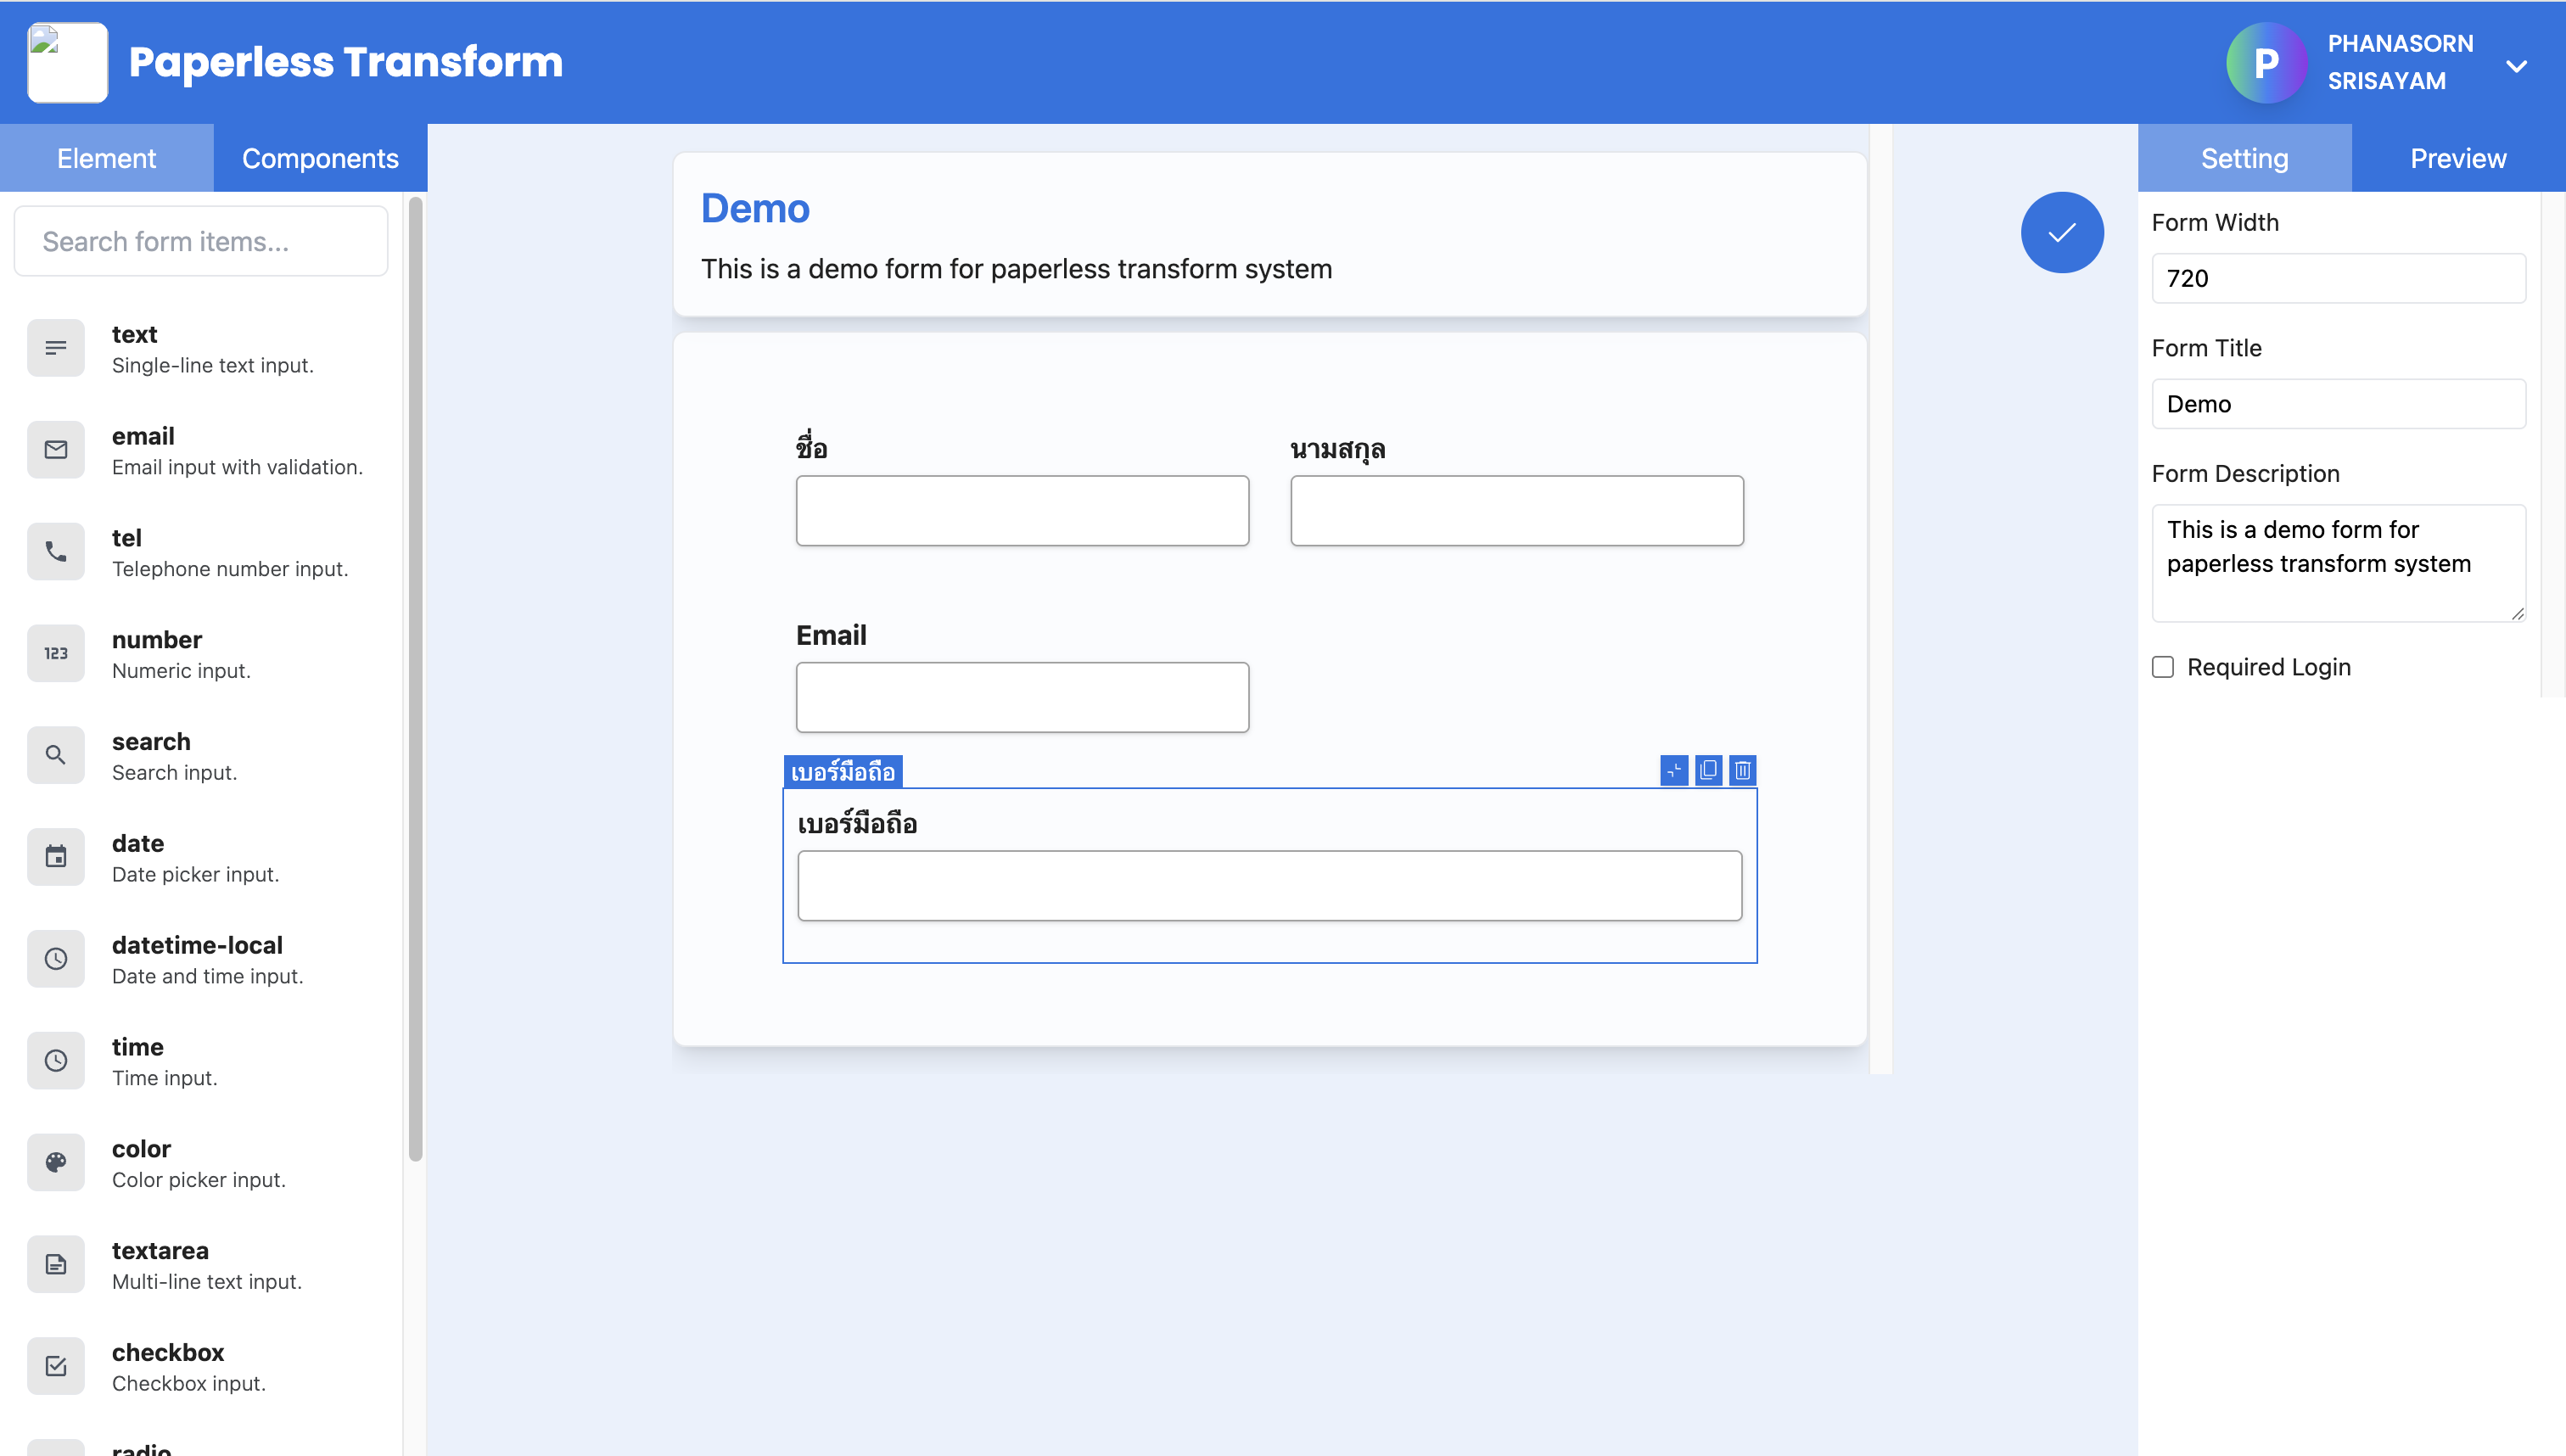
\includegraphics[width= 10cm]{./assets/UI/edit-form.png}}
\caption{Edit Form Page}\label{fig:edit-form}
\end{figure}

Figure \ref{fig:edit-form}  represents the Edit Form. The edit form page uses our own customize form editor based on Formkit, which allows users to fully customize a form, including changing input box length and add a input validation

\subsection{Form Page}

\begin{figure}[!h]
\centering
\fbox{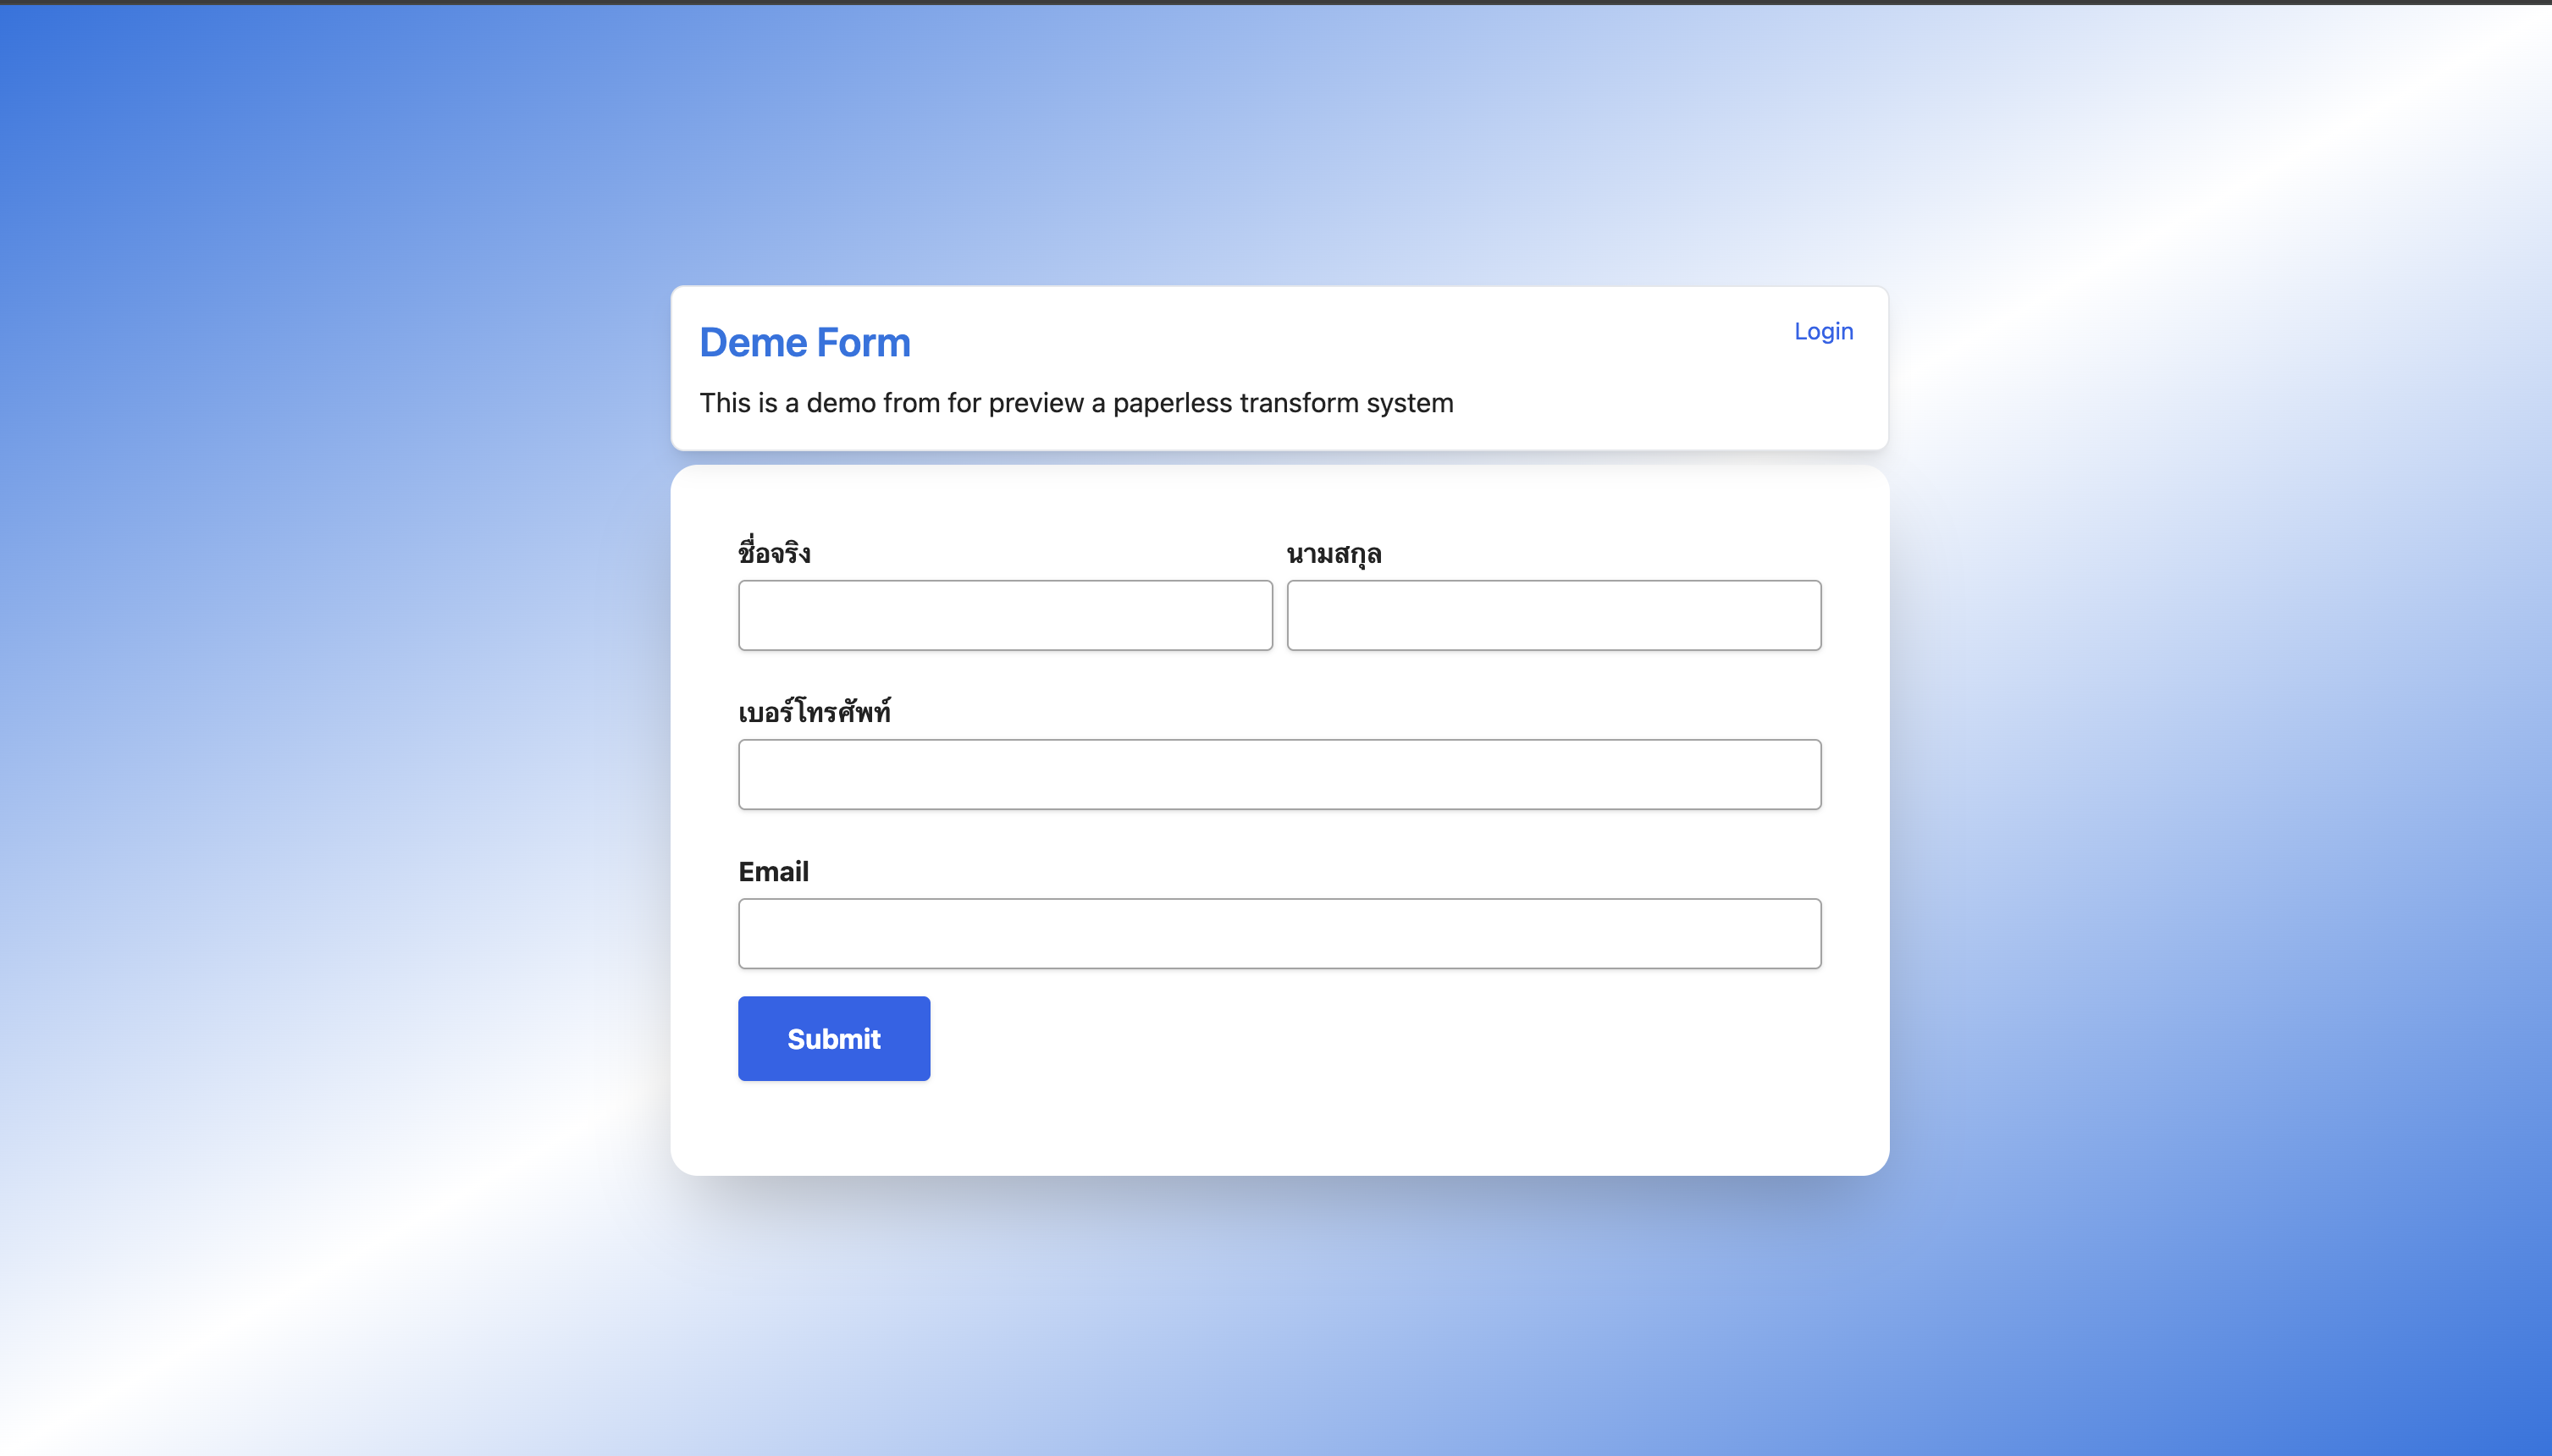
\includegraphics[width= 10cm]{./assets/UI/form-page.png}}
\caption{Form Page}\label{fig:form-page}
\end{figure}

Figure \ref{fig:form-page} showcases the example of web form user interface, which it use a surveyJS to render the UI. This  page will allow user to fill the information and submit a data to the system.


%%%%%%%%%%%%%%%%%%%%%%%%%%%%%%%%%%%%%%%%%%%%%%%%%%%%%%%%
%%%%%%%%%%%%%%%%%%%% Experiments %%%%%%%%%%%%%%%%%%%%%%%%%%%%%
%%%%%%%%%%%%%%%%%%%%%%%%%%%%%%%%%%%%%%%%%%%%%%%%%%%%%%%%
\chapter{Implementation Result}

This chapter will cover the entire working process and implementation progress of our project. Address complex issues as well. And we will divide each topic based on its features, which will include project data preparation.

\section{Data Preparation}

To study the structure of input fields and textual elements, approximately over 100 PDF forms were collected from various sources. These documents reflect a wide range of formatting styles and content arrangements, offering a diverse dataset for analysis. The findings from this analysis informed the development of methods for layout structure detection, text extraction, and input field identification. And we categorized the forms into three distinct styles based on input field presentation, which have dot-style forms, line-style forms, and tabular-style forms. And the following figure show the example of each form styles.

\begin{figure}[H]
\centering
\fbox{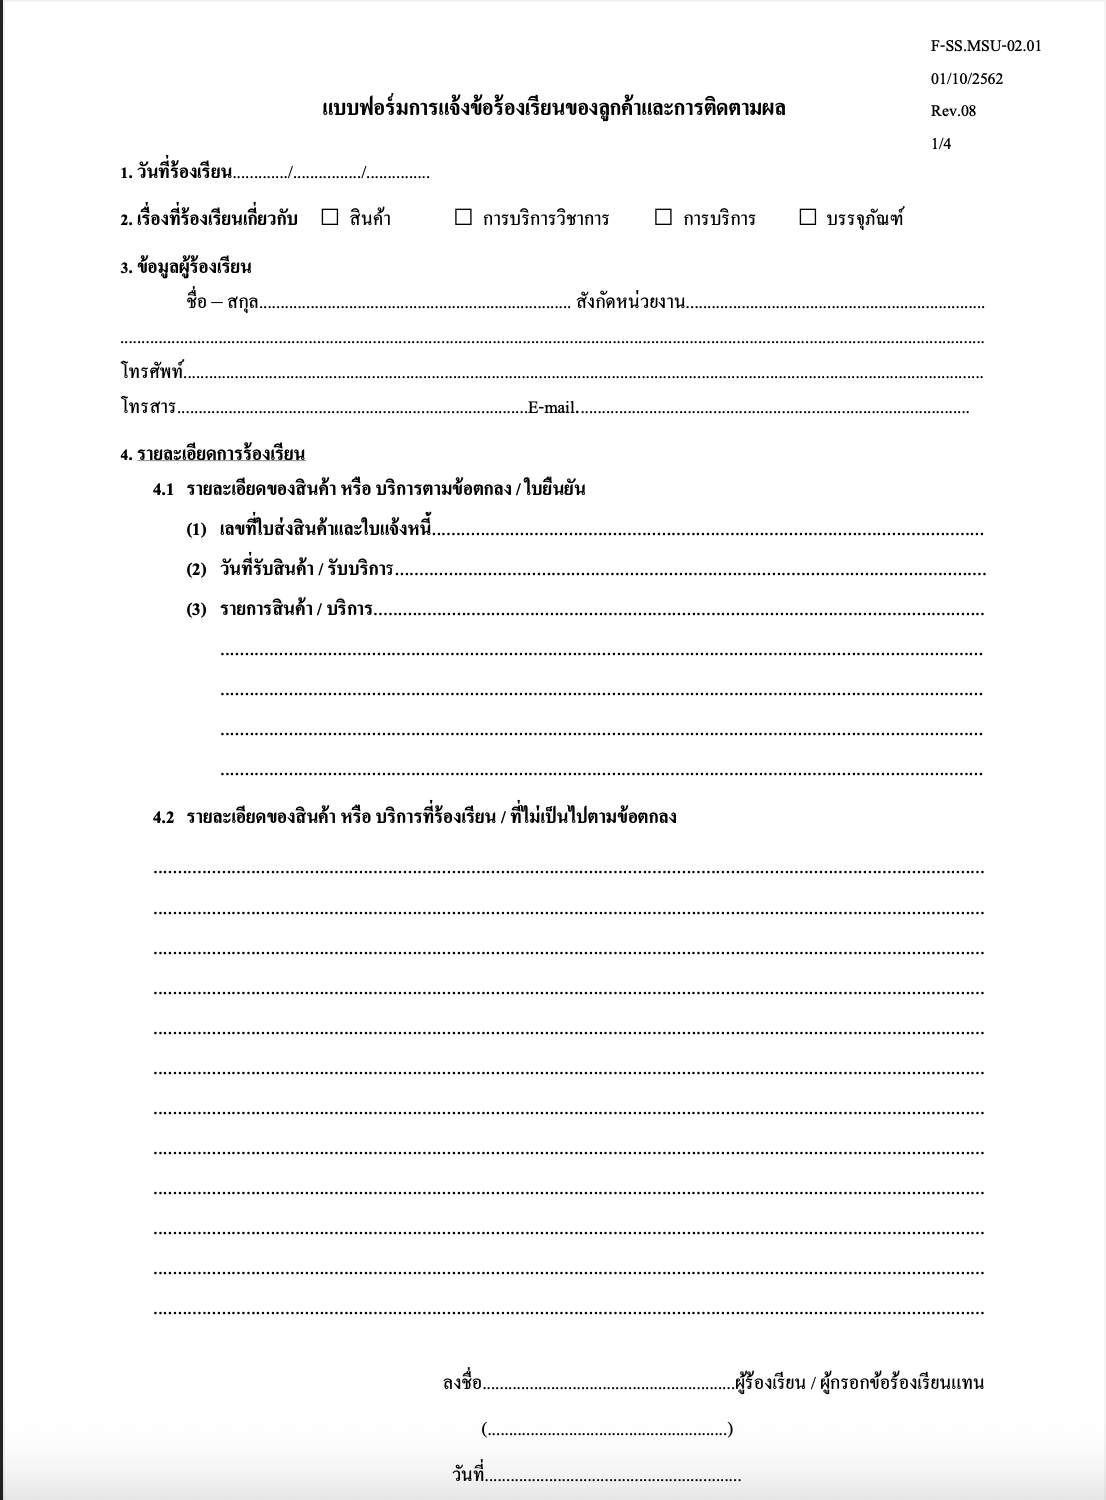
\includegraphics[width= 10cm]{./assets/dot-form.png}}
\caption{Example of dot-style forms}\label{fig:dot-form}
\end{figure}

\begin{figure}[H]
\centering
\fbox{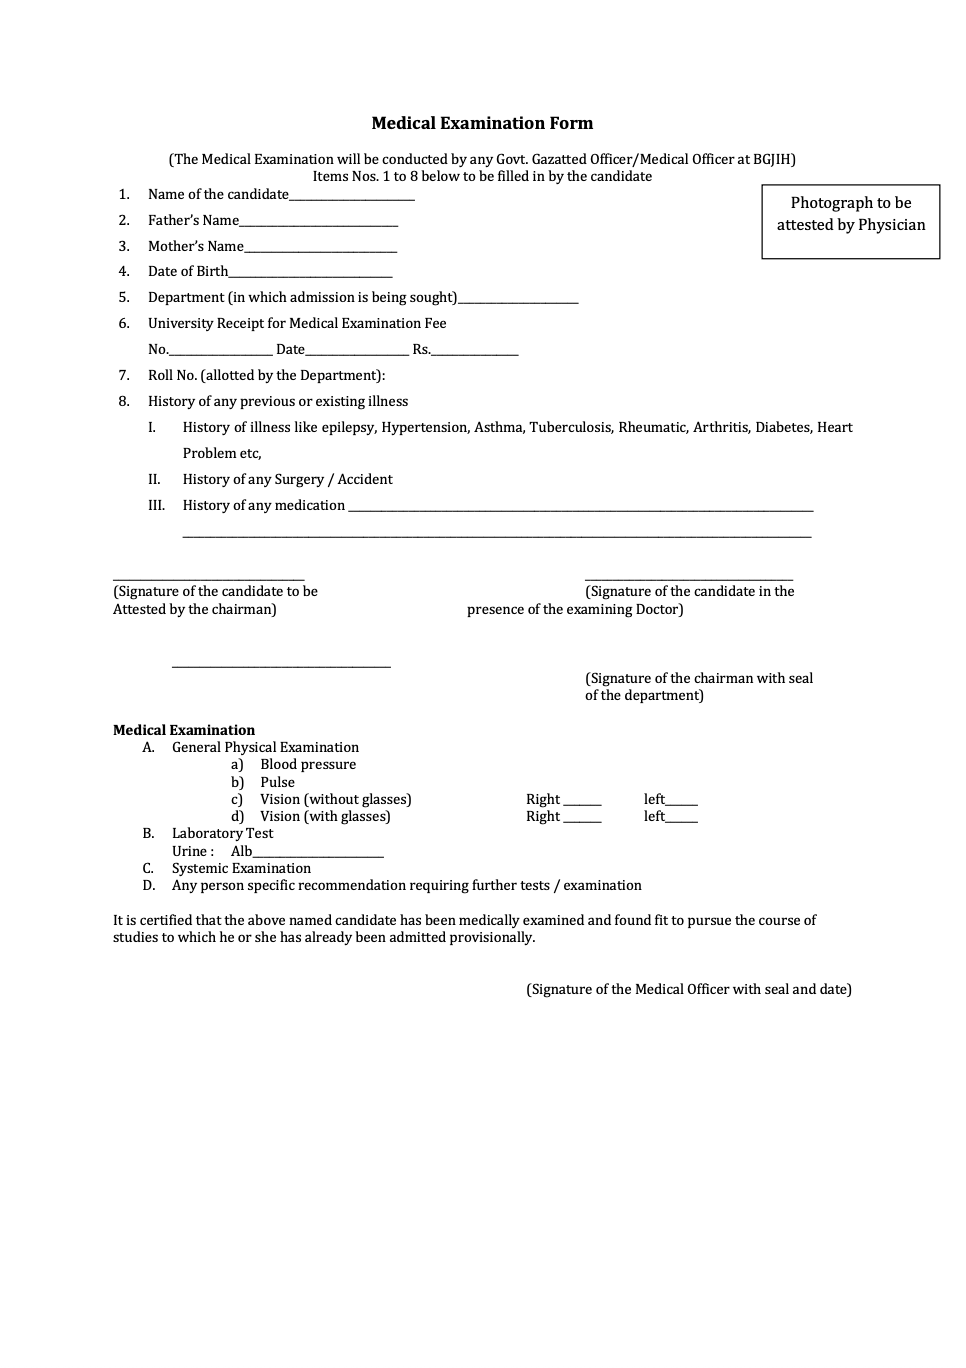
\includegraphics[width= 10cm]{./assets/line-form.png}}
\caption{Example of line-style forms}\label{fig:line-form}
\end{figure}

\begin{figure}[H]
\centering
\fbox{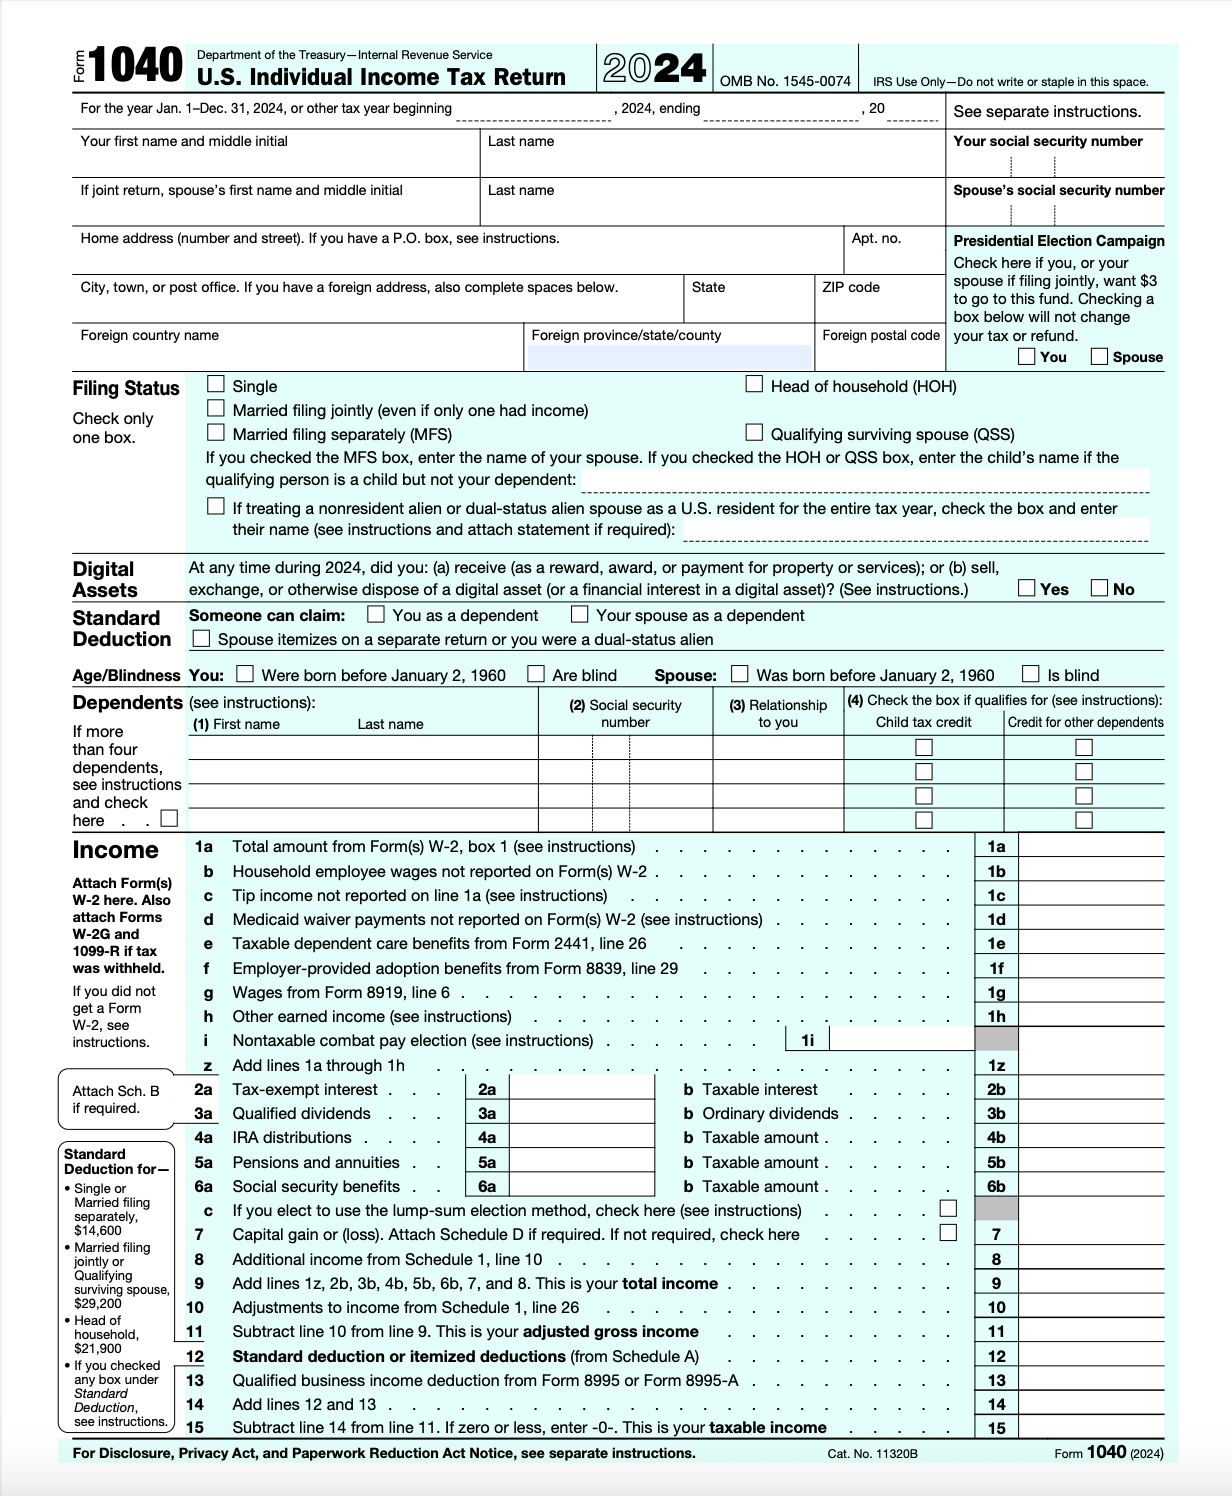
\includegraphics[width= 10cm]{./assets/tabular-form.png}}
\caption{Example of tabular-style forms}\label{fig:tabular-form}
\end{figure}

\section{Form Layout Analysis System}

The Paper-Based Form Analysis System is mainly focused on extracting a text from PDF file, and analyzing a form layout to identify an input label in the text, also the translation part and data type generator by using generative AI.

\subsection{Text Extraction Feature}

The Text Extraction Process has been implemented using PyMuPDF, a high-performance library. It is a library that facilitates the extraction, analysis, conversion, and manipulation of PDF data. The text extraction from the PDF file is illustrated in Figure \ref{fig:pdf-result}. However, there are still issues with the dot extraction process, as the dot character in some cases has multiple Unicode characters. To address this, we employ a text replacement algorithm to replace all potential dots with a standard dot or the Unicode character "U+002E" in order to normalize them. An additional issue is that a vowel in Thai text has been replaced with another character, such as {
\XeTeXlinebreaklocale "th_TH"	
\XeTeXlinebreakskip = 0pt plus 1pt
\thaifont
"ชื'อ"} when it should be {
\XeTeXlinebreaklocale "th_TH"	
\XeTeXlinebreakskip = 0pt plus 1pt
\thaifont
 ชื่อ."} Our research indicates that this issue is caused by the fact that the Unicode font is distinct from the standard font, and some may be the result of the compression of the PDF.

\begin{figure}[H]
\centering
\fbox{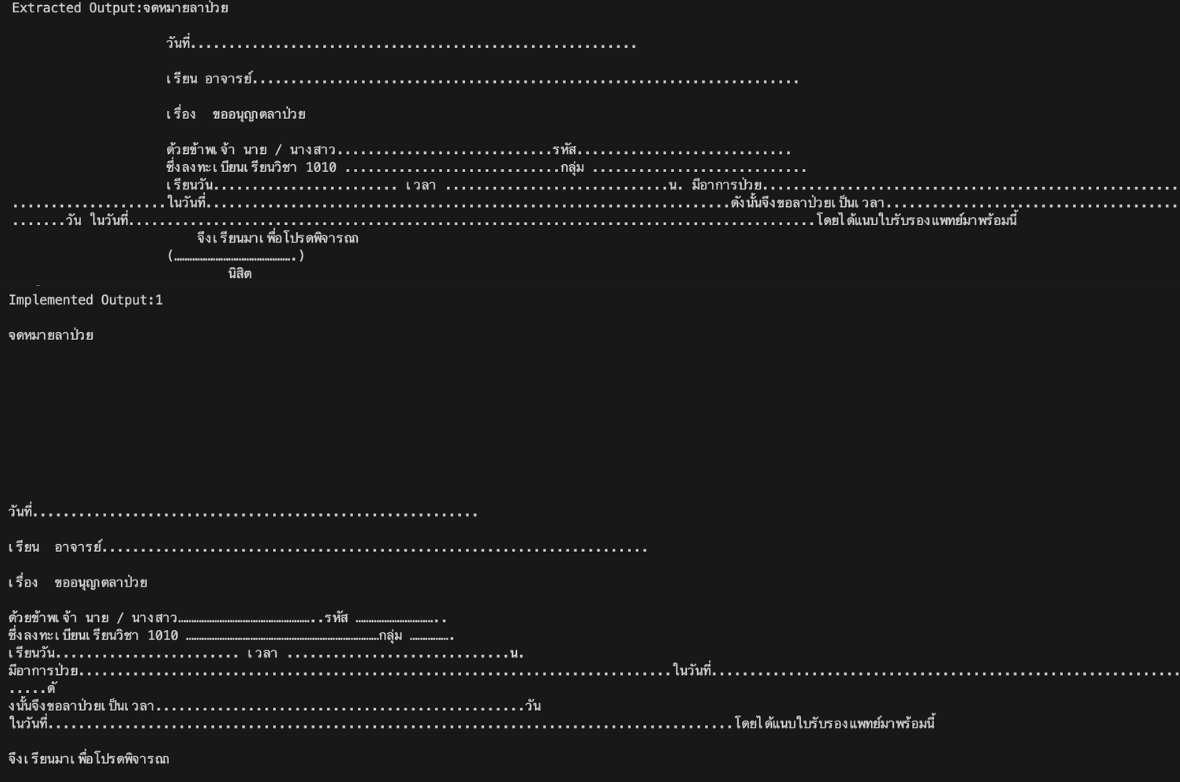
\includegraphics[width= 10cm]{./assets/pdf-extract.png}}
\caption{PDF Text Extraction Result}\label{fig:pdf-result}
\end{figure}

\subsection{Form Parser}
The Form Parse is implemented to identify an input label of the form and separate a form title. we have te

\begin{figure}[H]
\centering
\fbox{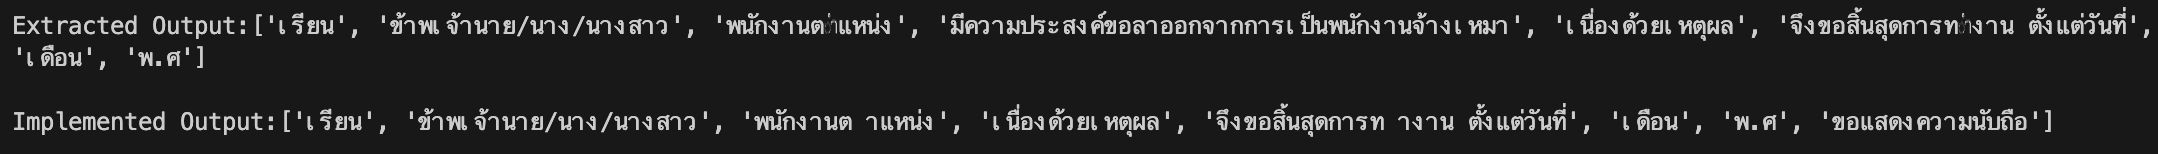
\includegraphics[width= 10cm]{./assets/form-parse.png}}
\caption{Form Parse Result}\label{fig:Form-Parse}
\end{figure}

\subsection{Translation Thai to English}
The Translation is use to translate a Thai language input label to english. we have use a NLLB-200 fined tuned model. Figure \ref{fig:trans-result} below show that the translation is working correctly but may not it may get a text that we expect, such as \textthai{วันเกิด} expected value to be Date of Birth, but the predicted result show "Birthdate". which it have ability to translate into a correct meaning.

\begin{figure}[H]
\centering
\fbox{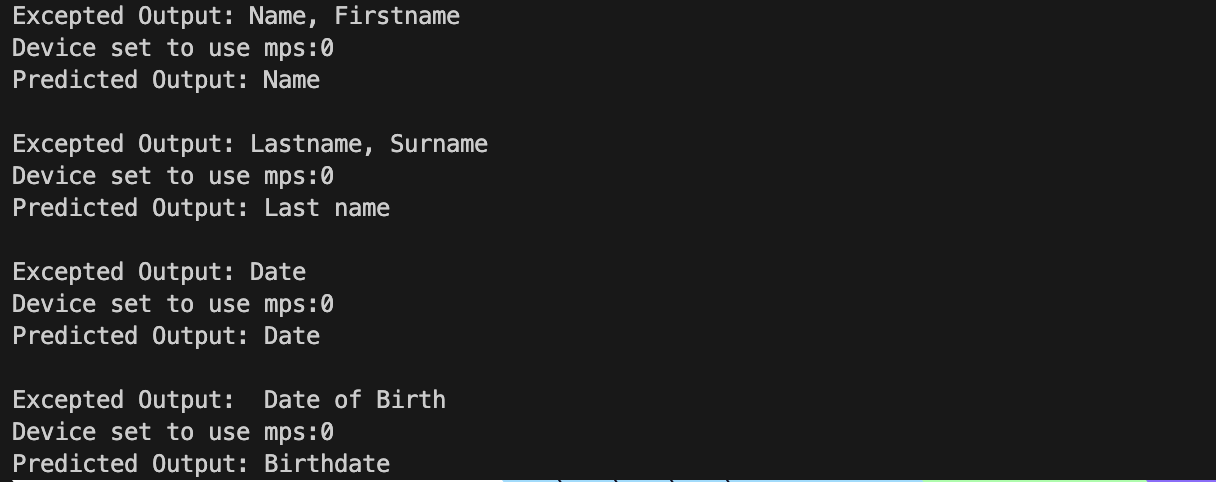
\includegraphics[width= 10cm]{./assets/translation-result.png}}
\caption{Translation Result}\label{fig:trans-result}
\end{figure}

\subsection{Data Type Analyzer}
Figure \ref{fig:datatype-result} has shown the 3 simple test case result that input the array of text and the system will generate a json as output. And it show a correct result for 1 and 2, but the 3 has failed because we have input a Thai text and some field are not correct as expect result.

\begin{figure}[H]
\centering
\fbox{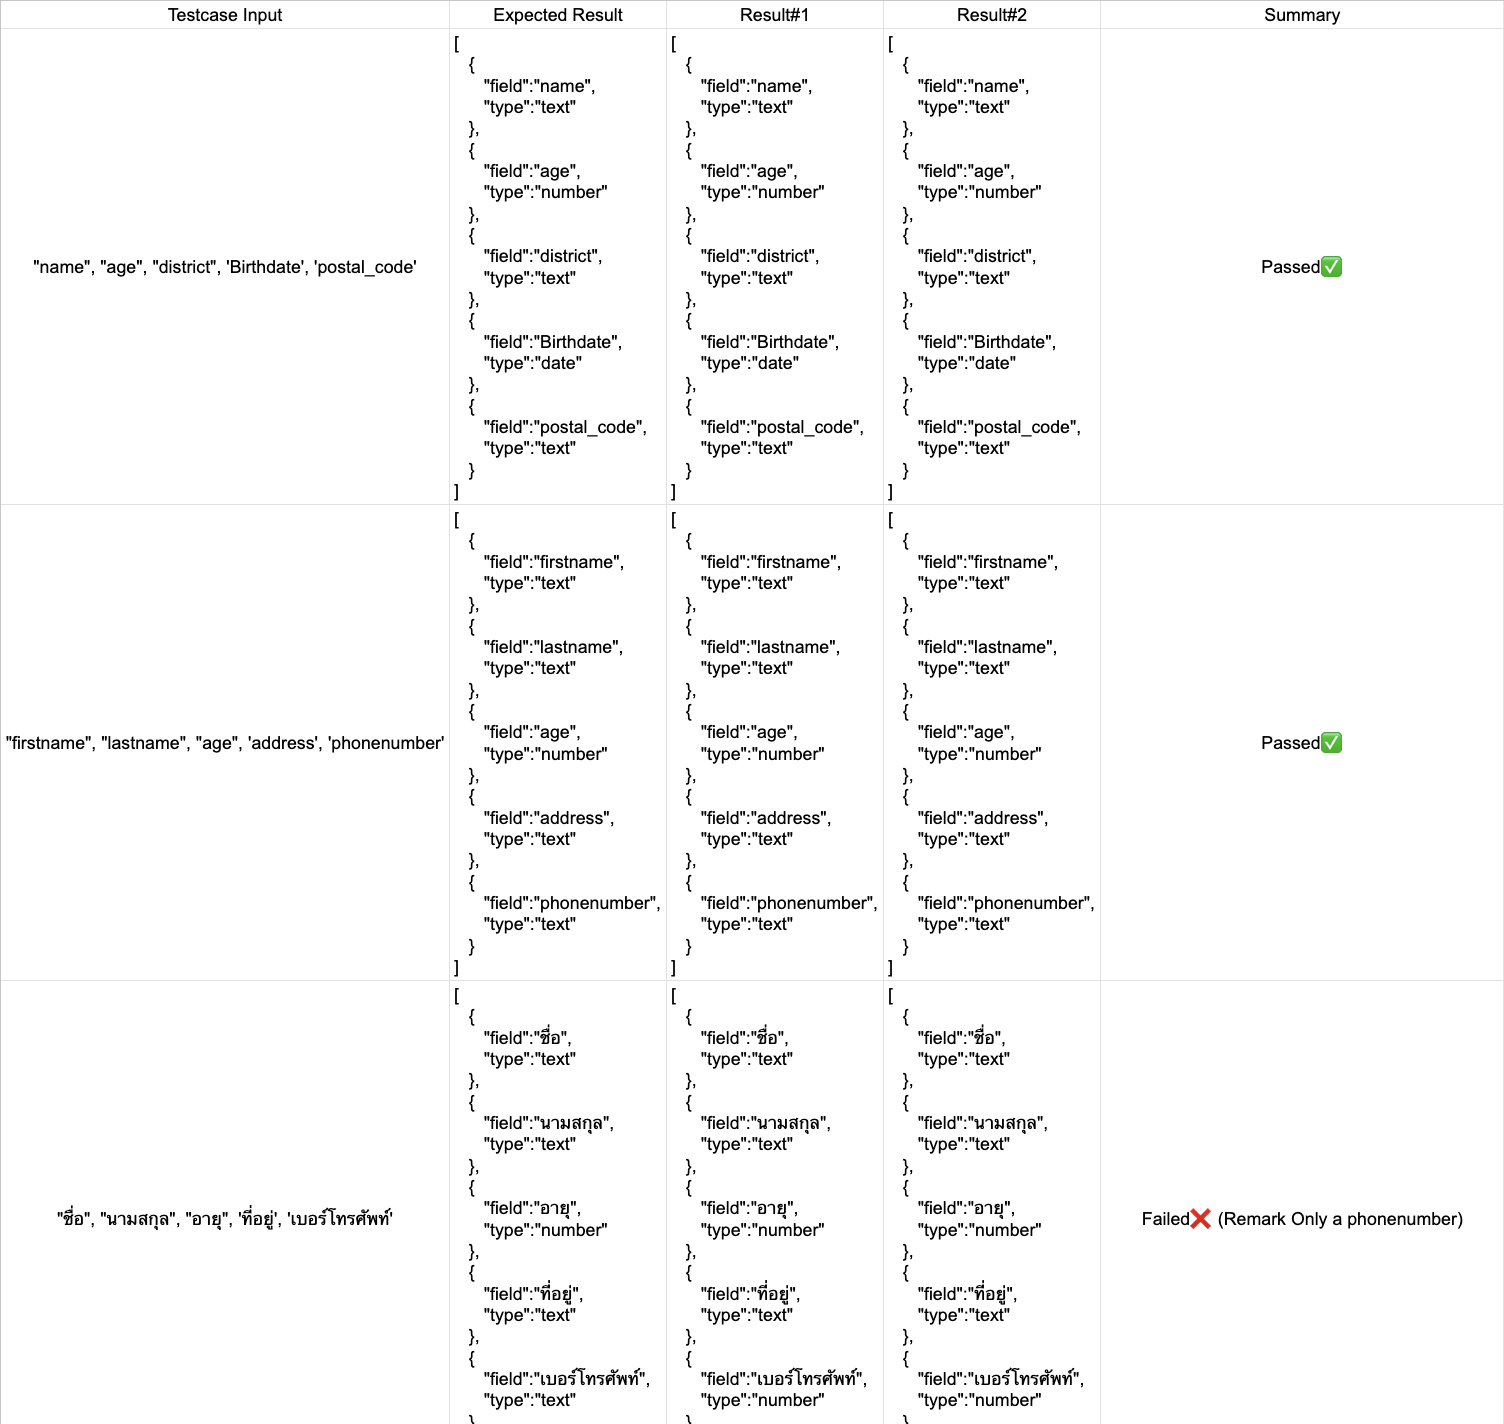
\includegraphics[width= 10cm]{./assets/datatype-result.png}}
\caption{Data Type Analyzer Result}\label{fig:datatype-result}
\end{figure}


\section{Web Application Implementation}

The web application development is progressing well, with significant milestones achieved in the front-end implementation and back-end implementation. The following features have been successfully developed and tested with a responsive user interface.

\subsection{Front-end development}

In this project, we developed a frontend application using Vue 3 with TypeScript, styled with Tailwind CSS for a modern design. We utilized Pinia for state management, ensuring efficient and scalable data handling across components. Axios was integrated for HTTP requests, enabling seamless communication with the backend API. This setup provides a modular, maintainable, and performant user interface, supporting features such as authentication, form management, and user profile handling.

\textbf{Authentication System:} Includes Login, Sign-Up, and Forgot Password pages.

\begin{figure}[H]
\centering
\fbox{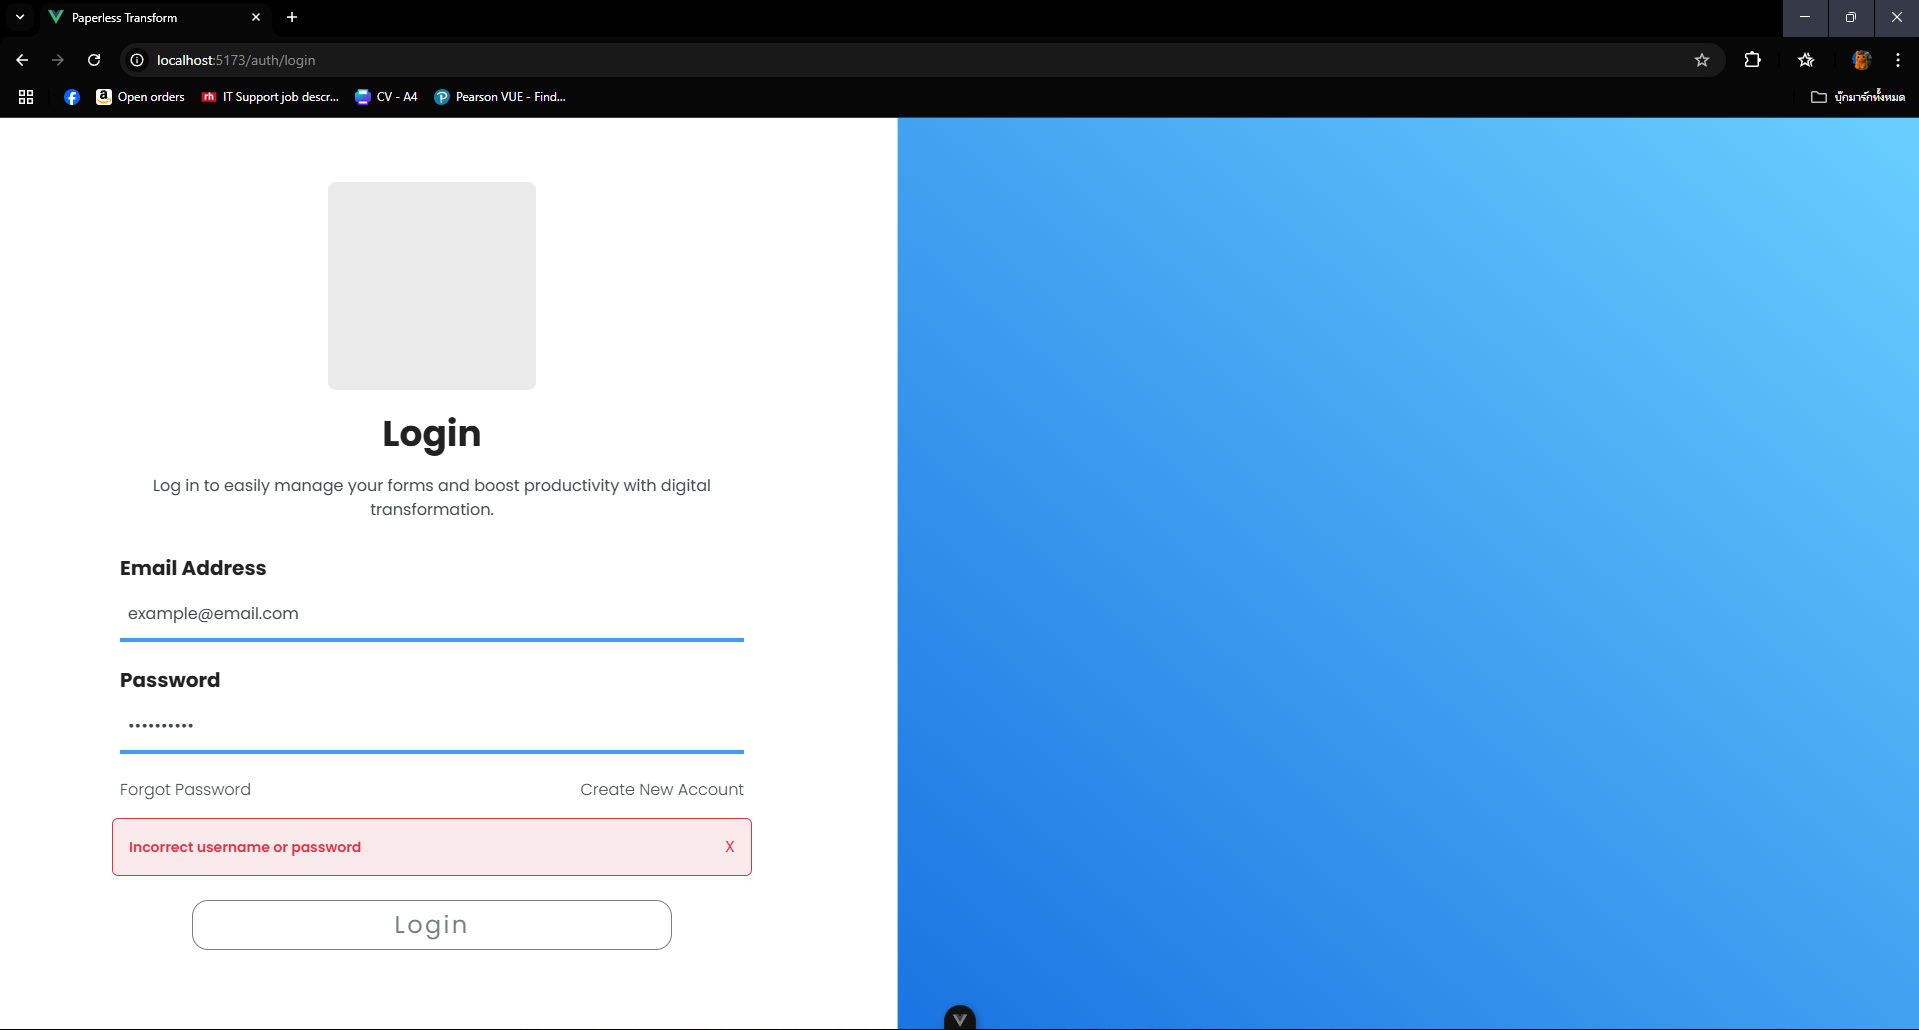
\includegraphics[width= 10cm]{./assets/auth-login.png}}
\caption{Implemented Login Page}\label{fig:auth-login}
\end{figure}

\begin{figure}[H]
\centering
\fbox{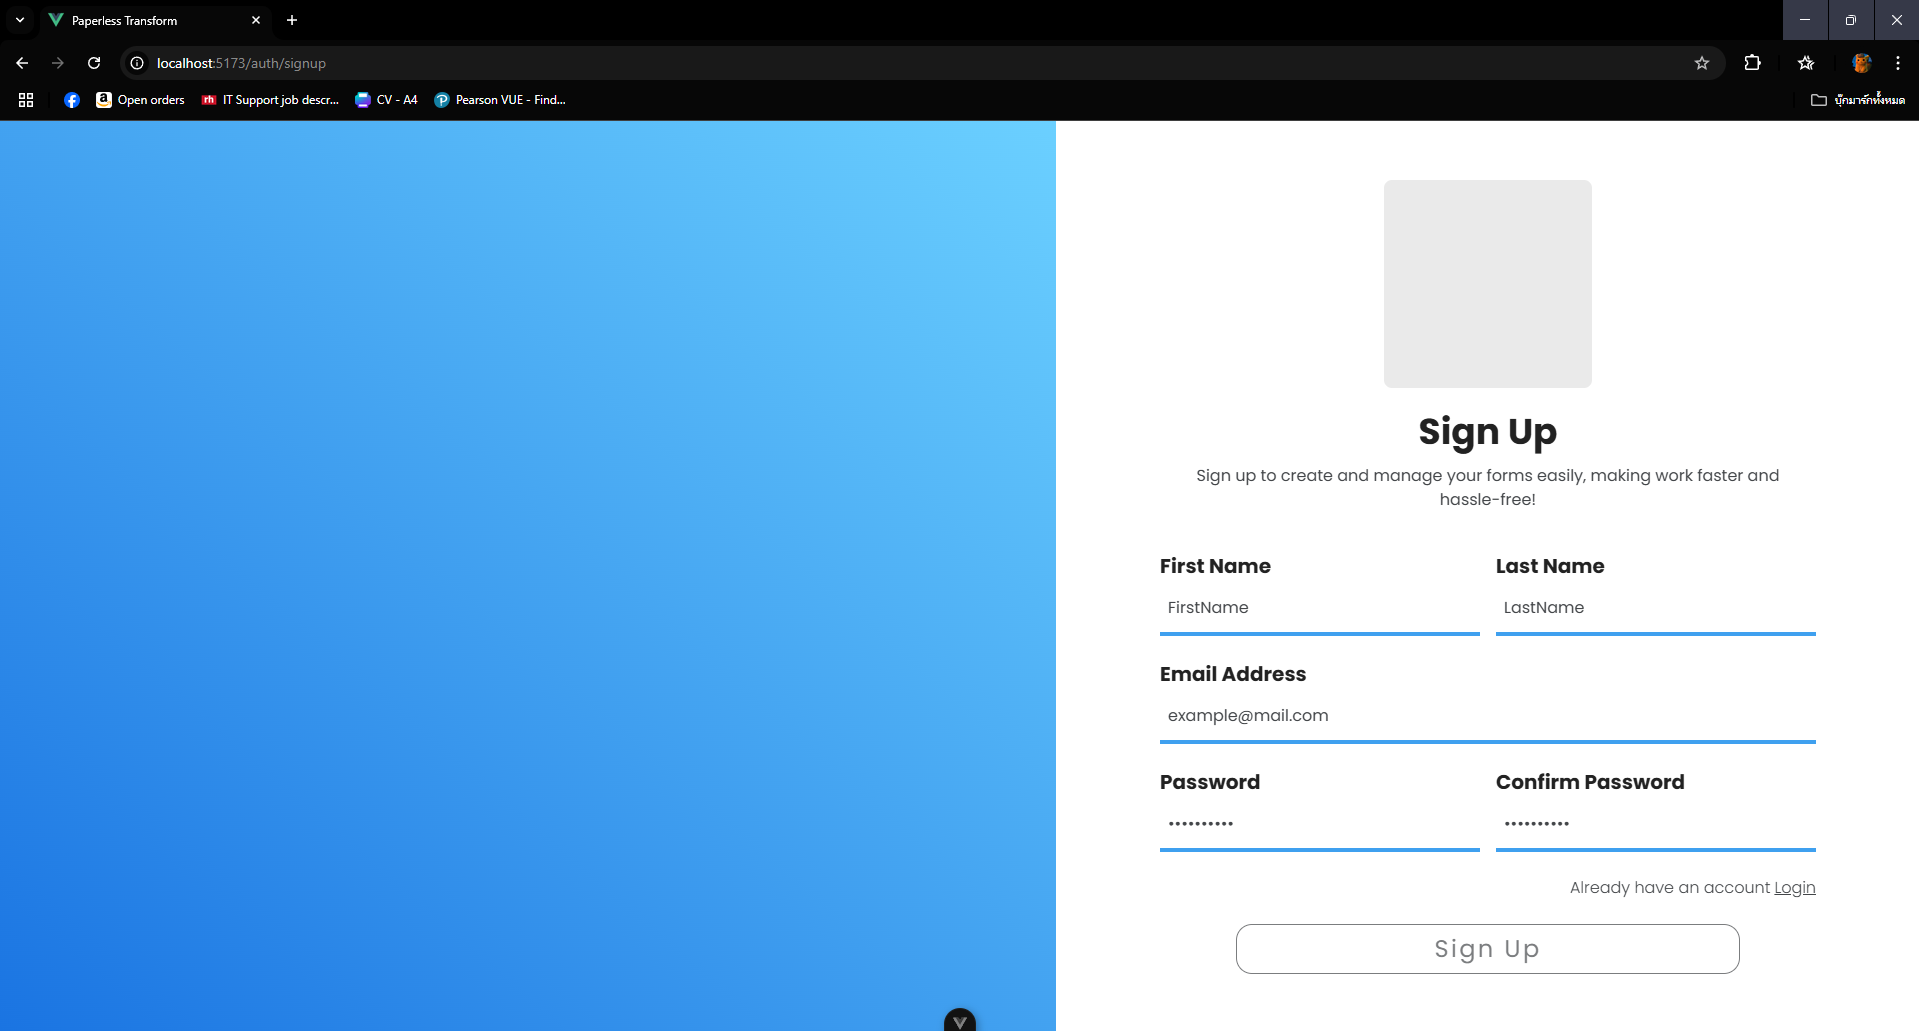
\includegraphics[width= 10cm]{./assets/auth-signup.png}}
\caption{Implemented Signup Page}\label{fig:auth-signup}
\end{figure}

\begin{figure}[H]
\centering
\fbox{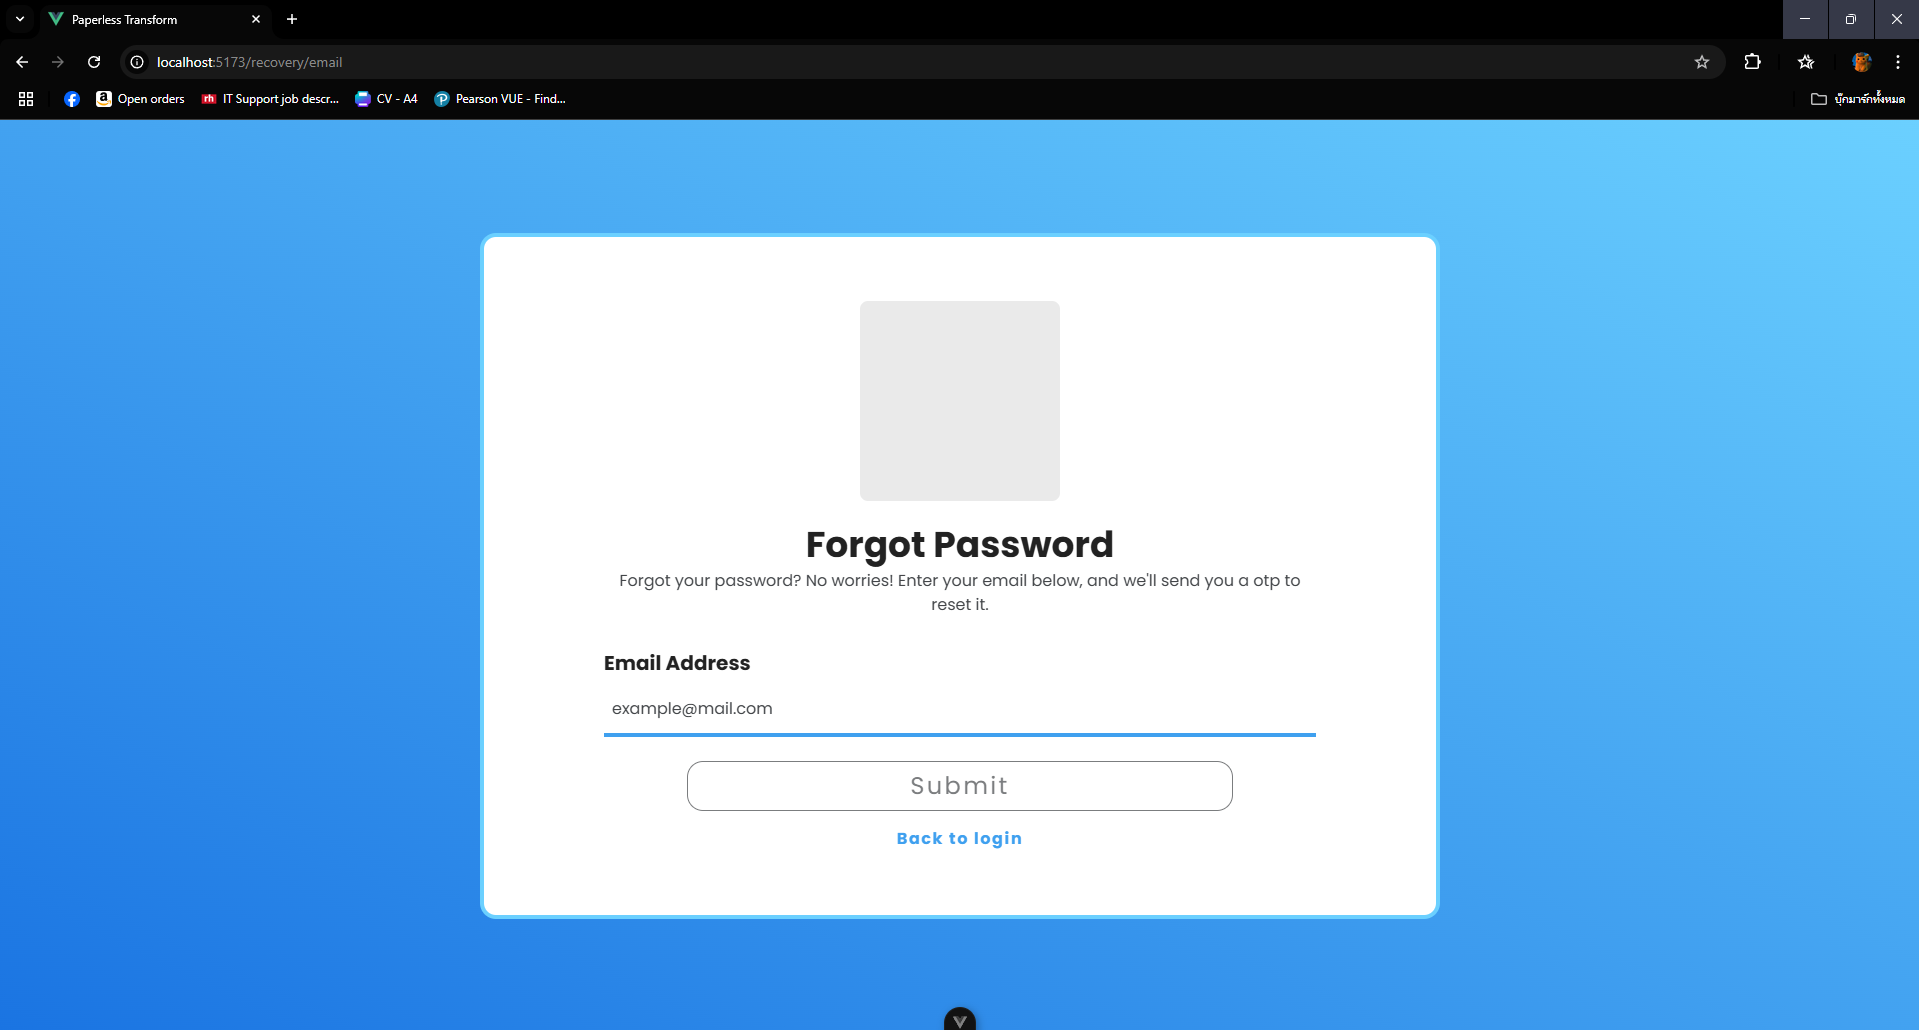
\includegraphics[width= 10cm]{./assets/auth-forgotpasswd.png}}
\caption{Implemented Forgot Passowrd}\label{fig:auth-forgotpasswd}
\end{figure}

\textbf{Dashboard Page:} Dashboard Page: Fully implemented with necessary functionalities,  such as upload files, status files upload, and recent form display with search by keyword.

\begin{figure}[H]
\centering
\fbox{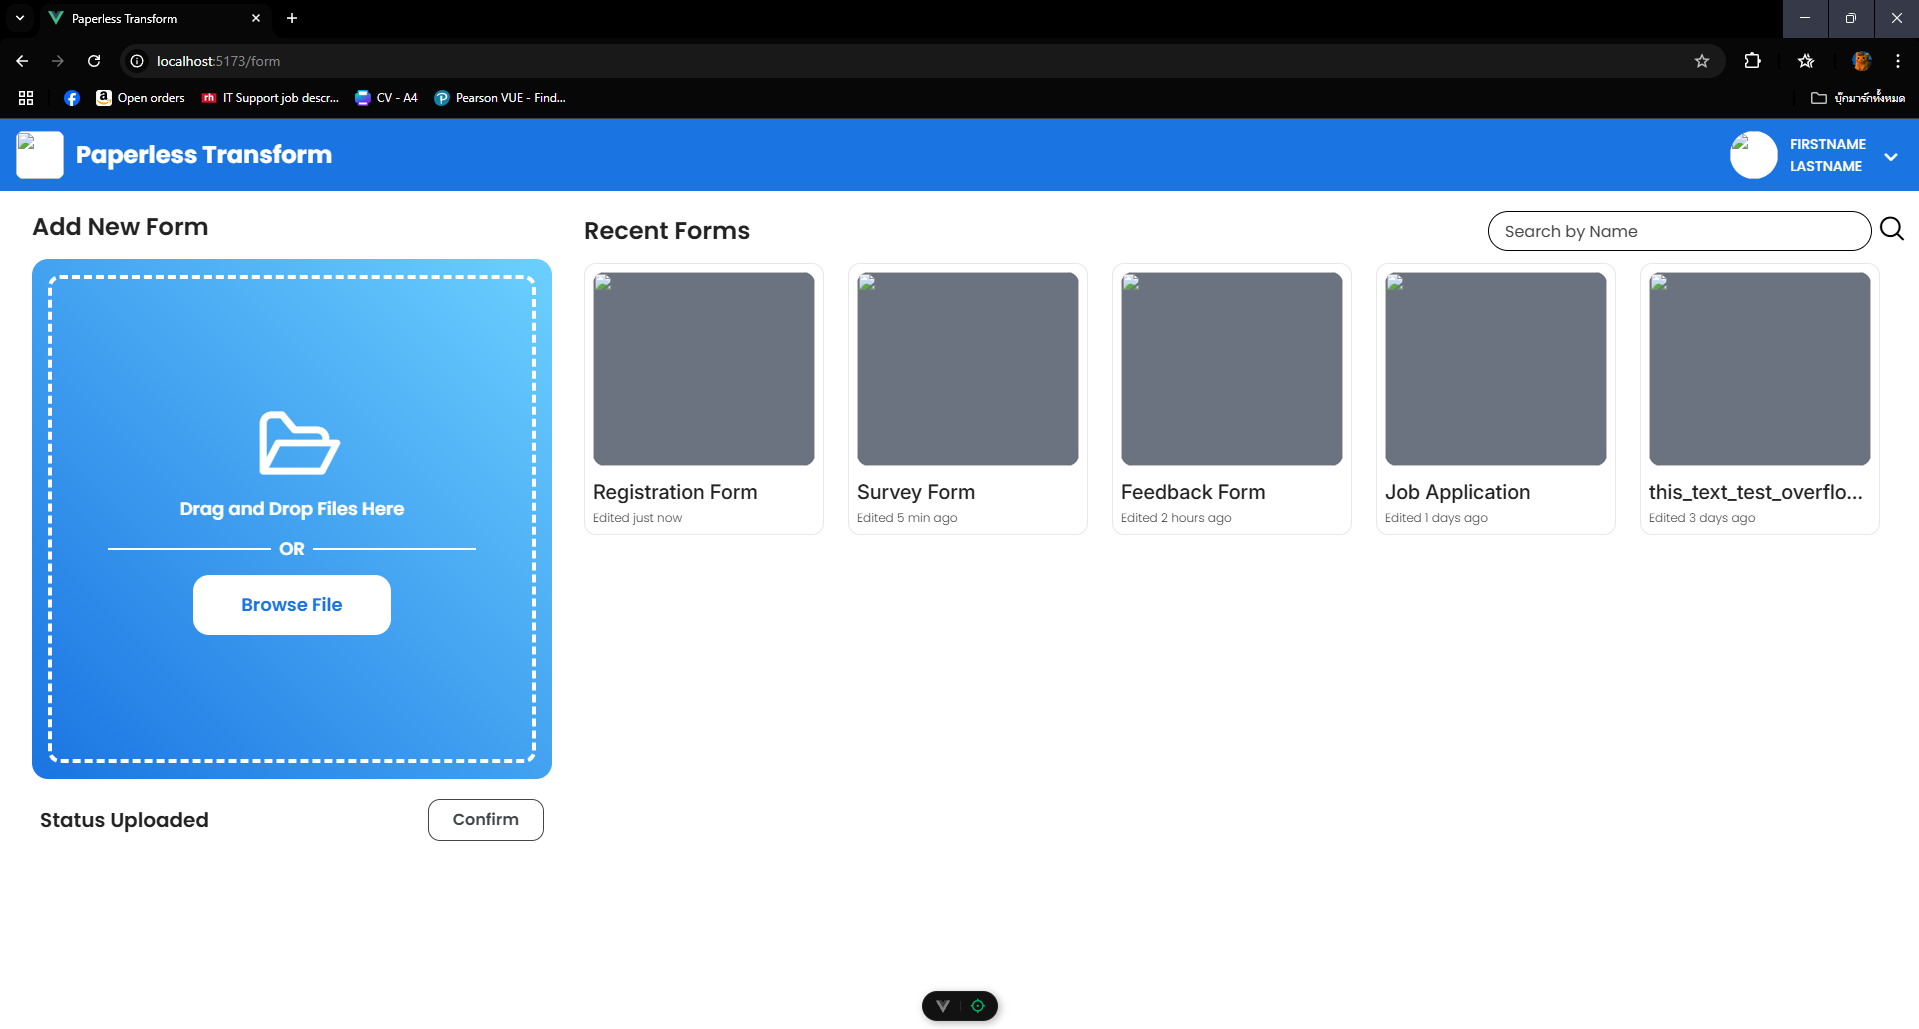
\includegraphics[width= 10cm]{./assets/dashboard.png}}
\caption{Implemented Dashboard Page}\label{fig:dashboard-result}
\end{figure}

\subsection{Back-end development}

In this process, we construct a FastAPI application to manage a user and form within a PostgreSQL database. We have written an API by using class programming and utilized Pydantic to create a model to validate and support data from incoming requests. We also implemented a SQLModel for object relation mapping to communicate with the PostgreSQL database. Additionally, we implemented a session management system with JWT.

The backend of the application is responsible for data manipulation, form management, and user authentication. It offers secure methods for user registration, login, password recovery, and profile management. Form creation, viewing, submission, and deletion are all supported by the API, which guarantees efficient data management. The routes are specifically designed to facilitate specific tasks, such as user authentication and form submission, while simultaneously guaranteeing data integrity and secure access. Efficient communication between the server and the frontend is facilitated by this infrastructure.


\begin{table}[h]
\centering
\caption{Page Route API Specification}
\begin{tabular}{|l|p{9cm}|c|}
\hline
\textbf{Route} & \textbf{Description} & \textbf{Method} \\
\hline
\texttt{/auth} & The main authentication route that redirects users to the login page if they are not logged in. It is a guest-only route, preventing access for logged-in users. & GET \\
\hline
\texttt{/auth/login} & The login page where users can enter their credentials (email and password) to access their account. & GET \\
\hline
\texttt{/auth/signup} & The registration page where new users can create an account by providing necessary information (email, password, and other details). & GET \\
\hline
\texttt{/recovery} & Password recovery section, redirecting users to the email submission page. This section is designed for users who have forgotten their passwords. & GET \\
\hline
\texttt{/recovery/email} & The email submission form for password recovery. Users provide their registered email to initiate the password reset process. & GET \\
\hline
\texttt{/recovery/otp} & The OTP (One-Time Password) verification page where users enter the verification code sent to their email for password recovery. & GET \\
\hline
\texttt{/recovery/reset} & The password reset form where users can set a new password after successful OTP verification. & GET \\
\hline
\texttt{/} & The main dashboard route (for authenticated users only). It redirects to the form dashboard, serving as the home page for logged-in users. & GET \\
\hline
\texttt{/form} & The form dashboard page displays a list of all available forms that users can access, or manage. & GET \\
\hline
\texttt{/form/result/:id} & The form result page displays the submitted data for a specific form identified by the ID in the URL. & GET \\
\hline
\texttt{/form/:id} & The form display page renders a specific form identified by the ID in the URL, allowing users to fill and submit the form. & GET \\
\hline
\texttt{/add} & The form builder page allows users to create new forms by designing form fields and layout, supporting customization and editing. & GET \\
\hline
\texttt{/profile} & The profile settings page allows users to view and update their personal information, such as name, email, and password. & GET \\
\hline
\texttt{/feedback} & The feedback submission page enables users to provide feedback on the system, sharing their experience and suggestions for improvement. & GET \\
\hline
\texttt{/aboutus} & The About Us page provides information about the project, its purpose, and the development team behind it. & GET \\
\hline
\end{tabular}
\label{tab:routes_overview}
\end{table}


\begin{table}[h]
\centering
\caption{Authentication Routes API Specification}
\begin{tabular}{|l|p{9cm}|c|}
\hline
\textbf{Route} & \textbf{Description} & \textbf{Method} \\
\hline
\texttt{/auth/signup} & Registers a new user with the provided input for sign-up. & POST \\
\hline
\texttt{/auth/signin} & Authenticates a user with the provided input for sign-in. & POST \\
\hline
\texttt{/auth/request-reset} & Initiates the password reset process by requesting a reset. & POST \\
\hline
\texttt{/auth/verify-otp} & Verifies the OTP for password reset process. & POST \\
\hline
\texttt{/auth/reset-password} & Resets the user password with the provided new password input. & POST \\
\hline
\end{tabular}
\label{tab:auth_post_routes}
\end{table}

\begin{table}[h]
\centering
\caption{Form and User Routes}
\begin{tabular}{|l|p{9cm}|c|}
\hline
\textbf{Route} & \textbf{Description} & \textbf{Method} \\
\hline
\texttt{/form} & Fetches a list of all available forms, allowing the user to view multiple forms that are currently stored in the system. & GET \\
\hline
\texttt{/form} & Creates a new form using the input data provided by the user. This allows for the addition of new forms to the system. & POST \\
\hline
\texttt{/form/:formId} & Deletes a form identified by the provided formId from the system. This action removes the form and its associated data. & DELETE \\
\hline
\texttt{/form/:formId/submit} & Submits the form data for a specific form identified by the formId. This operation processes and stores the data submitted through the form. & POST \\
\hline
\texttt{/form/:formId/result} & Retrieves the result data for a specific form, identified by the formId. This allows users to view the results or output generated after the form was submitted. & GET \\
\hline
\texttt{/user} & Fetches the details of the currently authenticated user. This route returns information about the user's profile, preferences, or other relevant data. & GET \\
\hline
\texttt{/user} & Update user detail & PATCH \\
\hline
\end{tabular}
\label{tab:form_user_routes}
\end{table}



%%%%%%%%%%%%%%%%%%%%%%%%%%%%%%%%%%%%%%%%%%%%%%%%%%%%%%%%%%%%%%%
%%%%%%%%%%%%%%%%%%%% Conclusions %%%%%%%%%%%%%%%%%%%%%%%%%%%%%
%%%%%%%%%%%%%%%%%%%%%%%%%%%%%%%%%%%%%%%%%%%%%%%%%%%%%%%%%%%%%%%
\chapter{Conclusions}

%THIS IS AN EXAMPLE. ALL SECTIONS BELOW ARE OPTIONAL. PLEASE CONSULT YOU ADVISOR AND DESIGN YOUR OWN SECTION

%\emph{\textthai{หัวข้อต่าง ๆ ในแต่ละบทเป็นเพียงตัวอย่างเท่านั้น หัวข้อที่จะใส่ในแต่ละบทขึ้นอยู่กับโปรเจคของนักศึกษาและอาจารย์ที่ปรึกษา}}

\section{Problems and Solutions}

\subsection{Lack of Optical Character Recognition}

From the outset, our objective was to create a system that could convert an image form into a web form. However, we encountered an issue with OCR accuracy, as the text that emerged from the OCR did not correspond to the text in the image. Nevertheless, the text parser is unable to extract a text label as a result of the OCR accuracy from the initial step. The text parser's main detection method is a dot, underscore, and dash, which are absent from the OCR-extracted text.To address this issue, we have decided to focus only a PDF file for transform into a web form and kept OCR for the future plan.

\subsection{Lack of PDF Extraction}

We have attempted to extract text from multiple forms and have observed that certain files contain vowels in the Thai language that have been replaced with numbers or special characters. The PDF itself displays the vowels correctly; however, when we extract the text using the library or manually copy the file, the result is an incorrect word containing a special character. In this instance, we conducted research and discovered that the vowel change was caused by a specific font, a special Unicode, or a compressed PDF file. To resolve this issue, we will verify the position of any unusual special text or number when the text is extracted. If it is identified, we will perform an error correction. However, this will be addressed in a future plan.

\subsection{Lack of Tabular form support}

One of the forms in the dataset we have gathered is tabular form style, which we are unable to support because the text parser we currently use only supports forms with lines and use a layout detection. We plan to support this in the future.

\subsection{Language model for generating answers}

Initially, we resolved to employ the open-source Llama 3.2:1B to perform the generating task in the design and methodology section. At first, we attempted to employ the open-source Llama 3.2; however, the output that was generated did not align with the instructions we provided. Resolution We have implemented a novel version of the generative AI, Llama 3:8B, which includes an eight billion parameter for training. The outcome has been satisfactory, as anticipated by the instructions we have provided.

\section {Workloads}

\begin{table}[H]
  \centering
  \caption{Workload and Progress Summary}
  \label{tbl:workload-and-progress-summary}
  \begin{tabular}{|p{8cm}|p{4cm}|}
    \hline
    \textbf{Workloads}    & \textbf{Progress} \\
    \hline
    \textbf{Research}                                   &                   \\
    Learn about generative AI model           & Completed         \\
    Learn about translation model            & Completed         \\
    Learn about text parser            & Completed         \\
    Learn about Python programming language             & Completed         \\
    Learn about Node.js                                 & Completed         \\
    Learn about Typescript                              & Completed         \\
    \hline
    \textbf{Design}                                     &                   \\
    Design a use case diagram                           & Completed         \\
    Design a system workflow                            & Completed         \\
    Design a user interface                             & Completed         \\
    \hline
    \textbf{Implement}                                  &                   \\
    Implement front-end                                 & Completed         \\
    Implement back-end                                  & Completed         \\
    Implement text extraction                                  & Completed        \\
    Implement text parser                                  & Improvement        \\
    Implement translation                                  & Completed         \\
    Implement Llama model                                  & Completed         \\
    \hline
    \textbf{Test}                                       &                   \\
    Manual testing                                        & Completed         \\
    \hline
    \textbf{Deployment}                                   &                   \\
    Deploy stability of server (front-end / back-end) & Completed       \\
    \hline
  \end{tabular}
\end{table}


\section{Future Works}

\begin{itemize}
  \item The use of OCR has been postponed due to the current limitations in OCR accuracy, which result in the extracted text failing to consistently correspond with the image content.  Instead, our current phase will be dedicated to the conversion of PDF files into web forms.  Future development plans will take into account the improvement of OCR performance and the integration of image-to-web form conversion.
  
  \item Implement a form detection to detect more layout and support a tabular.
  
  \item Implement multi-file upload support, allowing users to upload several documents at once.
\end{itemize}


%\section{Future Works}
%What could be done in the future to make your projects better.

%%%%%%%%%%%%%%%%%%%%%%%%%%%%%%%%%%%%%%%%%%%%%%%%%%%%%%%%%%%%%%%
%%%%%%%%%%%%%%%%%%%% Bibliography %%%%%%%%%%%%%%%%%%%%%%%%%%%%%
%%%%%%%%%%%%%%%%%%%%%%%%%%%%%%%%%%%%%%%%%%%%%%%%%%%%%%%%%%%%%%%

%%%% Comment this in your report to show only references you have
%%%% cited. Otherwise, all the references below will be shown.
%\nocite{*}
%% Use the kmutt.bst for bibtex bibliography style 
%% You must have cpe.bib and string.bib in your current directory.
%% You may go to file .bbl to manually edit the bib items.

% Sept, 2021 by Thanin
% improve url breaks to prevent unnecessary big white spaces in some cases
\makeatletter
\g@addto@macro{\UrlBreaks}{\UrlOrds}
\makeatother
% 

\bibliographystyle{kmutt}
\bibliography{string,cpe}

\end{document}
